

\newtoggle{inTableHeader}% Track if still in header of table
\toggletrue{inTableHeader}% Set initial value
\newcommand*{\StartTableHeader}{\global\toggletrue{inTableHeader}}%
\newcommand*{\EndTableHeader}{\global\togglefalse{inTableHeader}}%

% Redefine tabular to initialize \StartTableHeader at start and end
\let\OldTabular\tabular%
\let\OldEndTabular\endtabular%
\renewenvironment{tabular}{\StartTableHeader\OldTabular}{\OldEndTabular\StartTableHeader}%

 %The min, mid and max values
\newcommand*{\MinNumberA}{0.5}%
\newcommand*{\MidNumberA}{0.75}%
\newcommand*{\MaxNumberA}{1.0}%

%Apply the gradient macro
\newcommand{\ApplyGradientA}[1]{%
    %\IfDecimal{#1}{
  \iftoggle{inTableHeader}{#1}{
    \ifdim #1 pt > \MidNumberA pt
        \pgfmathsetmacro{\PercentColor}{max(min(100.0*(#1 - \MidNumberA)/(\MaxNumberA-\MidNumberA),100.0),0.00)} %
        \colorbox{green!\PercentColor!yellow}{#1}
    \else
        \pgfmathsetmacro{\PercentColor}{max(min(100.0*(\MidNumberA - #1)/(\MidNumberA-\MinNumberA),100.0),0.00)} %
        \colorbox{red!\PercentColor!yellow}{#1}
    \fi
  }
  %}{#1}
  }

   %The min, mid and max values
\newcommand*{\MinNumbera}{0.5}%
\newcommand*{\MidNumbera}{0.75}%
\newcommand*{\MaxNumbera}{1.0}%

%Apply the gradient macro
\newcommand{\ApplyGradienta}[1]{%
    %\IfDecimal{#1}{
  \iftoggle{inTableHeader}{#1}{
    \ifdim #1 pt > \MidNumbera pt
        \pgfmathsetmacro{\PercentColor}{max(min(100.0*(#1 - \MidNumbera)/(\MaxNumbera-\MidNumbera),100.0),0.00)} %
        \colorbox{red!\PercentColor!yellow}{#1}
    \else
        \pgfmathsetmacro{\PercentColor}{max(min(100.0*(\MidNumbera - #1)/(\MidNumbera-\MinNumbera),100.0),0.00)} %
        \colorbox{green!\PercentColor!yellow}{#1}
    \fi
  }
  %}{#1}
  }

 %The min, mid and max values
\newcommand*{\MinNumberB}{0.0}%
\newcommand*{\MidNumberB}{0.05}%
\newcommand*{\MaxNumberB}{0.1}%
  
%Apply the gradient macro
\newcommand{\ApplyGradientB}[1]{%
    %\IfDecimal{#1}{
  \iftoggle{inTableHeader}{#1}{
    \ifdim #1 pt > \MidNumberB pt
        \pgfmathsetmacro{\PercentColor}{max(min(100.0*(#1 - \MidNumberB)/(\MaxNumberB-\MidNumberB),100.0),0.00)} %
        \colorbox{red!\PercentColor!yellow}{#1}
    \else
        \pgfmathsetmacro{\PercentColor}{max(min(100.0*(\MidNumberB - #1)/(\MidNumberB-\MinNumberB),100.0),0.00)} %
        \colorbox{green!\PercentColor!yellow}{#1}
    \fi
  }
  %}{#1}
  }

%The min, mid and max values
\newcommand*{\MinNumberC}{0.5}%
\newcommand*{\MidNumberC}{0.75}%
\newcommand*{\MaxNumberC}{1.0}%
  
%Apply the gradient macro
\newcommand{\ApplyGradientC}[1]{%
    %\IfDecimal{#1}{
  \iftoggle{inTableHeader}{#1}{
    \ifdim #1 pt > \MidNumberC pt
        \pgfmathsetmacro{\PercentColor}{max(min(100.0*(#1 - \MidNumberC)/(\MaxNumberC-\MidNumberC),100.0),0.00)} %
        \colorbox{red!\PercentColor!yellow}{#1}
    \else
        \pgfmathsetmacro{\PercentColor}{max(min(100.0*(\MidNumberC - #1)/(\MidNumberC-\MinNumberC),100.0),0.00)} %
        \colorbox{green!\PercentColor!yellow}{#1}
    \fi
  }
  %}{#1}
  }

  
 %The min, mid and max values
\newcommand*{\MinNumberD}{0.5}%
\newcommand*{\MidNumberD}{0.75}%
\newcommand*{\MaxNumberD}{1.0}%

%Apply the gradient macro
\newcommand{\ApplyGradientD}[1]{%
    %\IfDecimal{#1}{
  \iftoggle{inTableHeader}{#1}{
    \ifdim #1 pt > \MidNumberD pt
        \pgfmathsetmacro{\PercentColor}{max(min(100.0*(#1 - \MidNumberD)/(\MaxNumberD-\MidNumberD),100.0),0.00)} %
        \colorbox{red!\PercentColor!yellow}{#1}
    \else
        \pgfmathsetmacro{\PercentColor}{max(min(100.0*(\MidNumberD - #1)/(\MidNumberD-\MinNumberD),100.0),0.00)} %
        \colorbox{green!\PercentColor!yellow}{#1}
    \fi
  }
  %}{#1}
  }
   %The min, mid and max values
\newcommand*{\MinNumberE}{0.5}%
\newcommand*{\MidNumberE}{0.75}%
\newcommand*{\MaxNumberE}{1.0}%

%Apply the gradient macro
\newcommand{\ApplyGradientE}[1]{%
    %\IfDecimal{#1}{
  \iftoggle{inTableHeader}{#1}{
    \ifdim #1 pt > \MidNumberE pt
        \pgfmathsetmacro{\PercentColor}{max(min(100.0*(#1 - \MidNumberE)/(\MaxNumberE-\MidNumberE),100.0),0.00)} %
        \colorbox{red!\PercentColor!yellow}{#1}
    \else
        \pgfmathsetmacro{\PercentColor}{max(min(100.0*(\MidNumberE - #1)/(\MidNumberE-\MinNumberE),100.0),0.00)} %
        \colorbox{green!\PercentColor!yellow}{#1}
    \fi
  }
  %}{#1}
  }
     %The min, mid and max values
\newcommand*{\MinNumberF}{0.5}%
\newcommand*{\MidNumberF}{0.75}%
\newcommand*{\MaxNumberF}{1.0}%

%Apply the gradient macro
\newcommand{\ApplyGradientF}[1]{%
    %\IfDecimal{#1}{
  \iftoggle{inTableHeader}{#1}{
    \ifdim #1 pt > \MidNumberF pt
        \pgfmathsetmacro{\PercentColor}{max(min(100.0*(#1 - \MidNumberF)/(\MaxNumberF-\MidNumberF),100.0),0.00)} %
        \colorbox{red!\PercentColor!yellow}{#1}
    \else
        \pgfmathsetmacro{\PercentColor}{max(min(100.0*(\MidNumberF - #1)/(\MidNumberF-\MinNumberF),100.0),0.00)} %
        \colorbox{green!\PercentColor!yellow}{#1}
    \fi
  }
  %}{#1}
  }
     %The min, mid and max values
\newcommand*{\MinNumberG}{0.5}%
\newcommand*{\MidNumberG}{0.75}%
\newcommand*{\MaxNumberG}{1.0}%

%Apply the gradient macro
\newcommand{\ApplyGradientG}[1]{%
    %\IfDecimal{#1}{
  \iftoggle{inTableHeader}{#1}{
    \ifdim #1 pt > \MidNumberG pt
        \pgfmathsetmacro{\PercentColor}{max(min(100.0*(#1 - \MidNumberG)/(\MaxNumberG-\MidNumberG),100.0),0.00)} %
        \colorbox{green!\PercentColor!yellow}{#1}
    \else
        \pgfmathsetmacro{\PercentColor}{max(min(100.0*(\MidNumberG - #1)/(\MidNumberG-\MinNumberG),100.0),0.00)} %
        \colorbox{red!\PercentColor!yellow}{#1}
    \fi
  }
  %}{#1}
  }
     %The min, mid and max values
\newcommand*{\MinNumberg}{0.5}%
\newcommand*{\MidNumberg}{0.75}%
\newcommand*{\MaxNumberg}{1.0}%

%Apply the gradient macro
\newcommand{\ApplyGradientg}[1]{%
    %\IfDecimal{#1}{
  \iftoggle{inTableHeader}{#1}{
    \ifdim #1 pt > \MidNumberg pt
        \pgfmathsetmacro{\PercentColor}{max(min(100.0*(#1 - \MidNumberg)/(\MaxNumberg-\MidNumberg),100.0),0.00)} %
        \colorbox{red!\PercentColor!yellow}{#1}
    \else
        \pgfmathsetmacro{\PercentColor}{max(min(100.0*(\MidNumberg - #1)/(\MidNumberg-\MinNumberg),100.0),0.00)} %
        \colorbox{green!\PercentColor!yellow}{#1}
    \fi
  }
  %}{#1}
  }


     %The min, mid and max values
\newcommand*{\MinNumberH}{0.5}%
\newcommand*{\MidNumberH}{0.75}%
\newcommand*{\MaxNumberH}{1.0}%

%Apply the gradient macro
\newcommand{\ApplyGradientH}[1]{%
    %\IfDecimal{#1}{
  \iftoggle{inTableHeader}{#1}{
    \ifdim #1 pt > \MidNumberH pt
        \pgfmathsetmacro{\PercentColor}{max(min(100.0*(#1 - \MidNumberH)/(\MaxNumberH-\MidNumberH),100.0),0.00)} %
        \colorbox{red!\PercentColor!yellow}{#1}
    \else
        \pgfmathsetmacro{\PercentColor}{max(min(100.0*(\MidNumberH - #1)/(\MidNumberH-\MinNumberH),100.0),0.00)} %
        \colorbox{green!\PercentColor!yellow}{#1}
    \fi
  }
  %}{#1}
  }



\newcolumntype{A}{>{\collectcell\ApplyGradientA}c<{\endcollectcell}}
\newcolumntype{a}{>{\collectcell\ApplyGradienta}c<{\endcollectcell}}
\newcolumntype{B}{>{\collectcell\ApplyGradientB}c<{\endcollectcell}}
\newcolumntype{C}{>{\collectcell\ApplyGradientC}c<{\endcollectcell}}
\newcolumntype{D}{>{\collectcell\ApplyGradientD}c<{\endcollectcell}}
\newcolumntype{E}{>{\collectcell\ApplyGradientE}c<{\endcollectcell}}
\newcolumntype{F}{>{\collectcell\ApplyGradientF}c<{\endcollectcell}}
\newcolumntype{G}{>{\collectcell\ApplyGradientG}c<{\endcollectcell}}
\newcolumntype{g}{>{\collectcell\ApplyGradientg}c<{\endcollectcell}}
\newcolumntype{H}{>{\collectcell\ApplyGradientH}c<{\endcollectcell}}

\renewcommand{\arraystretch}{1}
\setlength{\fboxsep}{2mm} % box size
\setlength{\tabcolsep}{-4pt}

\chapter{Výsledky}
\label{kap:results}

V tejto kapitole odprezentujeme výsledky dosiahnuté pri triangulácii konečných aj 
nekonečných, ohraničených plôch. Označme počet trojuholníkov vo výslednej triangulácii 
ako $n$ a počet vrcholov $p$.

\section{Kritéria kvality výslednej triangulácie}
\begin{enumerate}
\item{
    \textit{Priemerná dĺžka hrany}

    Pri zmenšovaní hrany vznikajú body $x_{proj}$ bližšie k povrchu, preto je ich premietanie
    presnejšie. Vzniknuté premietnuté trojuholníky majú preto dĺžku hrany bližšiu k zadanej dĺžke 
    $a$. Pre naše modely odmeriame priemernú dĺžku hrany a porovnáme ju so zadanou dĺžkou hrany $a$. 
    Dané porovnanie vyjadríme 
    pomerom, na ktorom budeme sledovať, či sa pri zmenšujúcej zadanej dĺžke $a$ približuje k $1$.

    Kritérium budeme označovať $k_1$.
}
\item{
    \textit{Vzdialenosť ťažiska od kolmého priemetu ťažiska}

    Zmenšovaním veľkosti hrany by sa mala priemerná vzdialenosť ťažiska od svojho kolmého 
    priemetu zmenšovať. Budeme sledovať pomer priemernej 
    vzdialenosti a zadanej dĺžky hrany $a$. Ak sa tento pomer pri zmenšujúcej sa dĺžke hrany 
    $a$ zmenšuje, vzdialenosť
    ťažiska od svojho priemetu klesá rýchlejšie ako dĺžka zadanej hrany $a$.

    Kritérium budeme označovať $k_2$.
}
\item{
    \textit{Pomer dĺžok strán trojuholníka}

    Zmenšovaním veľkosti hrany by malo vznikať viac takmer rovnostranných trojuholníkov.
    Dôvodom je, že menšie trojuholníky dokážu plochu presnejšie aproximovať aj v oblastiach 
    s väčším zakrivením. Preto sa trojuholníky nemusia nevhodne spájať a vytvárať množstvo 
    úzkych trojuholníkov. Opísanú vlastnosť budeme merať ako pomer dĺžok strán trojuholníka. 

    Odmeriame priemerný pomer najväčšej a najmenšej strany a budeme sledovať, či sa pri 
    zmenšujúcej dĺžke $a$ zmenšuje, resp. blíži zhora k $1$.

    Kritérium budeme označovať $k_3$.
}
\item{
    \textit{Diskrétna aproximácia Hausdorffovej vzdialenosti}

    \begin{definition}
        Nech $a \in \mathbb{R}^3$ je bod a $M \subset \mathbb{R}^3$ je množina.
        Vzdialenosť $\delta$ bodu $a$ od množiny $M$ definujeme ako
        \begin{equation}
            %\label{eq:point_set_distance}
            \delta(a, M) = \inf_{b \in M} \, d(a, b),
        \end{equation}
        pričom $d(a, b) = \sqrt{(a_x-b_x)^2 + (a_y-b_y)^2 + (a_z-b_z)^2}$ je euklidovská 
        vzdialenosť dvoch bodov v $\mathbb{R}^3$.
    \end{definition}

    \begin{definition}
        Nech $M \in \mathbb{R}^3, N \in \mathbb{R}^3$ sú množiny.
        Hausdorffovu vzdialenosť množín $N$ a $M$ definujeme ako
        \begin{equation}
            h(M, N) = \max \big \{\sup_{a \in M} \, \delta(a, N), \sup_{b \in N} \, \delta(M, b) \big \}.
        \end{equation}
    \end{definition}

    Ak sú množiny uzavreté, môžeme zjednodušene povedať, že pre každý bod z množiny $M$ nájdeme 
    vzdialenosť najbližšieho bodu z množiny $N$.
    Takisto aj pre každý bod z množiny $N$ nájdeme vzdialenosť najbližšieho bodu z množiny $M$.
    Následne z týchto vzdialeností vyberieme najväčšiu, túto vzdialenosť označíme ako 
    \textit{Hausdorffovu vzdialenosť}.

    Na obrázku \ref{obr:hausdorff_distance} vidíme ilustráciu \textit{Hausdorffovej vzdialenosti} 
    na troch dvojiciach množín.

    \begin{figure}
        \centerline{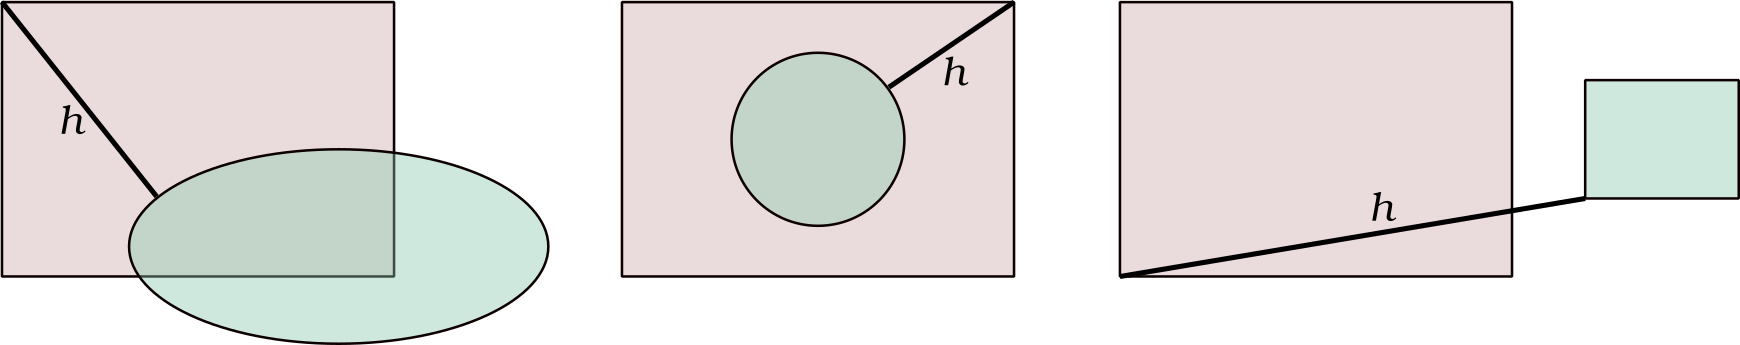
\includegraphics[width=1\textwidth]{images/Hausdorff_distance}}
        \caption[Hausdorffova vzdialenosť]{Hausdorffova vzdialenosť.}
        %id obrazku, pomocou ktoreho sa budeme na obrazok odvolavat
        \label{obr:hausdorff_distance}
    \end{figure}


    Pre nekonečné množiny bodov $M$ a $N$ túto vzdialenosť numericky aproximujeme na konečnej 
    podmnožine bodov $M$ a $N$. Keďže všetky vrcholy meshu ležia so zvolenou presnosťou na ploche, 
    predpokladáme, že body meshu, ktoré sú najvzdialenejšie od plochy sú ťažiská trojuholníkov.
    Ďalej predpokladáme, že najbližší bod z plochy k ťažisku trojuholníka triangulácie
    je kolmý priemet ťažiska na túto plochu.

    Potom diskrétnu numerickú aproximáciu \textit{Hausdorffovej vzdialenosti} definujeme nasledovne.
    \begin{definition}
        Nech $F:\mathbb{R}^3 \to \mathbb{R}$ je funkcia a $S = \{x \in \mathbb{R}^3 \, | \, F(x)=0 \}$ 
        je plocha. Nech $M$ je triangulácia plochy $S$
        a T je množina ťažísk trojuholníkov triangulácie $M$.
        Diskrétnou aproximáciou Hausdorffovej vzdialenosti nazveme vzdialenosť
        \begin{equation}
            h_d = \max_{t \in T} \big \{ d(t, t_{proj})\big \},
        \end{equation}
        pričom $t_{proj}$ je priemet bodu $t$ na plochu $S$ v smere vektora $\nabla F(t)$ a
        $d(a, b)$ je euklidovská vzdialenosť v $\mathbb{R}^3$.
    \end{definition}

    Pre zmenšujúcu sa veľkosť hrany očakávame zmenšujúcu sa \textit{diskrétnu Hausdorffovu vzdialenosť}.
    Opäť budeme sledovať aj pomer $h_d : a$. Ak tento pomer pri zmenšovaní dĺžky $a$ klesá, potom 
    \textit{diskrétna Hausdorffova vzdialenosť} klesá rýchlejšie ako zmenšujúca sa dĺžka $a$.

    Kritérium budeme označovať $k_4$.
}
\item{
    \textit{Minimálny a maximálny uhol normál susedných trojuholníkov}

    Keďže $F$ je regulárna plocha, pre zmenšujúcu sa zadanú dĺžku $a$ by sa mal minimálny aj maximálny 
    uhol normál susedných trojuholníkov triangulácie blížiť k nule. Samozrejme, povrchom, ktoré majú 
    v niektorých oblastiach vyššie zakrivenie klesá maximálny uhol normál oveľa pomalšie ako minimálny
    uhol. Toto správanie sa pokúsime sledovať aj na našich modeloch.

    Kritériá budeme označovať $k_5$ (minimálny uhol) a $k_6$ (maximálny uhol).
}
\item{
    \textit{Priemerná vzdialenosť susedných vrcholov od vrchola meshu a smerodajná odchýlka tejto vzdialenosti od priemeru}

    Smerodajná odchýlka hovorí o rozložení hodnôt okolo priemeru. Čím je smerodajná odchýlka menšia, 
    tým bližšie sú hodnoty k priemeru. Naopak, ak je smerodajná odchýlka väčšia, tak sú hodnoty okolo
    priemeru viac rozptýlené.
    
    Majme $N$ hodnôt. Nech $\overline{x}$ označuje aritmetický priemer. 
    Smerodajnú odchýlku môžeme vypočítať podľa nasledujúceho vzorca.

    \begin{equation}
    \label{eq:std}
    \sigma = \sqrt{\frac{1}{N} \sum\limits_{i=1}^{N}(x_i - \overline{x})^2} 
    \end{equation}

    Pre zmenšujúcu sa veľkosť hrany očakávame rovnomerne rozložené vrcholy. Preto očakávame, že 
    priemerná vzdialenosť sa bude blížiť k dĺžke hrany $a$ a smerodajná odchýlka sa bude zmenšovať.
    
    Pre naše modely odmeriame priemer z týchto priemerných vzdialeností (ozn. $p_p$)a takisto priemer 
    zo smerodajných odchýliek (ozn $p_s$). Očakávame, že pomer $p_p : a$ sa bude so zmenšujúcim sa $a$
    blížiť k $1$ a pomer $p_s : a$ sa bude blížiť k $0$.

    Kritériá budeme označovať $k_7$ (priemer) a $k_8$ (smerodajná odchýlka).
}
\end{enumerate}

\section{Meranie}

V tejto kapitole odprezentujeme výsledky meraní kritérií kvality na ôsmych konečných plochách
a šiestich nekonečných plochách využívajúc ohraničujúcu obálku.
Pre konečné plochy pozorujeme modely pre 5 rôznych zadaných dĺžok hrán, pre nekonečné ohraničené plochy pre
4 rôzne zadané dĺžky hrán. Ku každej ploche sme vytvorili tabuľku s nameranými kritériami. 

V stĺpci $k_1$ môžeme pozorovať výsledky merania kritéria $k_1$. Vo všetkých modeloch jasne vidíme, 
že pomer priemernej dĺžky hrany ku zadanej dĺžke hrany sa pre zmenšujúce sa $a$ pribižuje k $1$.

V stĺpci $k_2$ pozorujeme zmenšujúci sa pomer priemernej vzdialenosti ťažiska od svojho priemetu ku 
zadanej dĺžke hrany. Teda pri zmenšujúcej sa zadanej dĺžke $a$, vzdialenosť ťažiska od svojho priemetu 
klesá rýchlejšie ako zadaná dĺžka hrany.

V stĺpci $k_3$ pozorujeme priemerný pomer najdlhšej strany trojuholníka ku najkratšej. Ako sme očakávali,
tento priemer sa približuje k jednej, teda trojuholníky \textit{meshu} sú pre zmenšujúcu sa zadanú dĺžku hrany
$a$ čoraz viac pravidelné.

V stĺpci $k_4$ môžeme pozorovať diskrétnu aproximáciu Hausdorffovej vzdialenosti v pomere k zadanej dĺžke 
hrany $a$. Vidíme, že aj tento pomer väčšinou klesá, avšak napríklad pri \textit{tetrahdrone} môžeme 
pozorovať občasný výkyv. To je spôsobené tým, že nemeriame priemer ale maximum, čiže na výkyv stačí jeden 
trojuholník so vzdialenejším ťažiskom. 

V stĺpcoch $k_5$ a $k_6$ pozorujeme minimálny, resp. maximálny uhol normál susedných trojuholníkov.
Kvôli nízkym nameraným hodnotám, minimálny uhol zapisujeme do tabuľky ako stonásobok nameranej hodnoty. Aj 
pri týchto kritériách pozorujeme občasné výkyvy. Pri maximálnom uhle sú tieto výkyvy z rovnakého dôvodu
ako pri kritériu $k_4$. Pri minimálnom uhle skôr tým, že takmer v každom modeli existuje dvojica trojuholníkov
s takmer nulovým uhlom normál. Potom ak model takúto dvojicu nemá, tak aj veľmi malý uhol sa zdá v porovnaní s takmer
nulovým príliš veľký.

V stĺpci $k_7$ a $k_8$ pozorujeme priemer priemerej vzdialenosti susedných bodov a priemer smerodajnej odchýlky 
tejto vzdialenosti v pomere k zadanej dĺžke hrany $a$. Ako sme očakávali, v stĺpci $k_7$ vidíme, že sa hodnoty pomeru
blížia k $1$ a v stĺpci $k_8$ sa blížia k $0$. To znamená, že v modeloch s menšou zadanou dĺžkou hrany $a$ sú 
vrcholy rozmiestnené rovnomernejšie, ako v modeloch s väčšou zadanou dĺžkou hrany $a$.

Po skončení algoritmu pre dostatočne malú veľkosť hrany vznikajú korektné triangulácie,
bez prekrývania trojuholníkov a taktiež bez dier.
\newpage
\subsection{Konečné plochy}

\begin{enumerate}
\item{
    \textit{Sféra}
    \begin{equation}
    \label{eq:sphere}
    x^2 + y^2 + z^2 - 1 = 0
    \end{equation}

    Na obrázku \ref{obr:sphere} vidíme výslednú trianguláciu sféry danej implicitnou 
    rovnicou \ref{eq:sphere} s piatimi rôznymi dĺžkami strany $a$.
    \begin{enumerate}[a)]
    \item{
        $a=0.900$, $n=64$, $p=34$
    }
    \item{
        $a=0.700$, $n=90$, $p=47$
    }
    \item{
        $a=0.500$, $n=160$, $p=82$
    }
    \item{
        $a=0.300$, $n=408$, $p=206$
    }
    \item{
        $a=0.100$, $n=3246$, $p=1625$
    }
    \end{enumerate}

    \begin{figure}
        \centerline{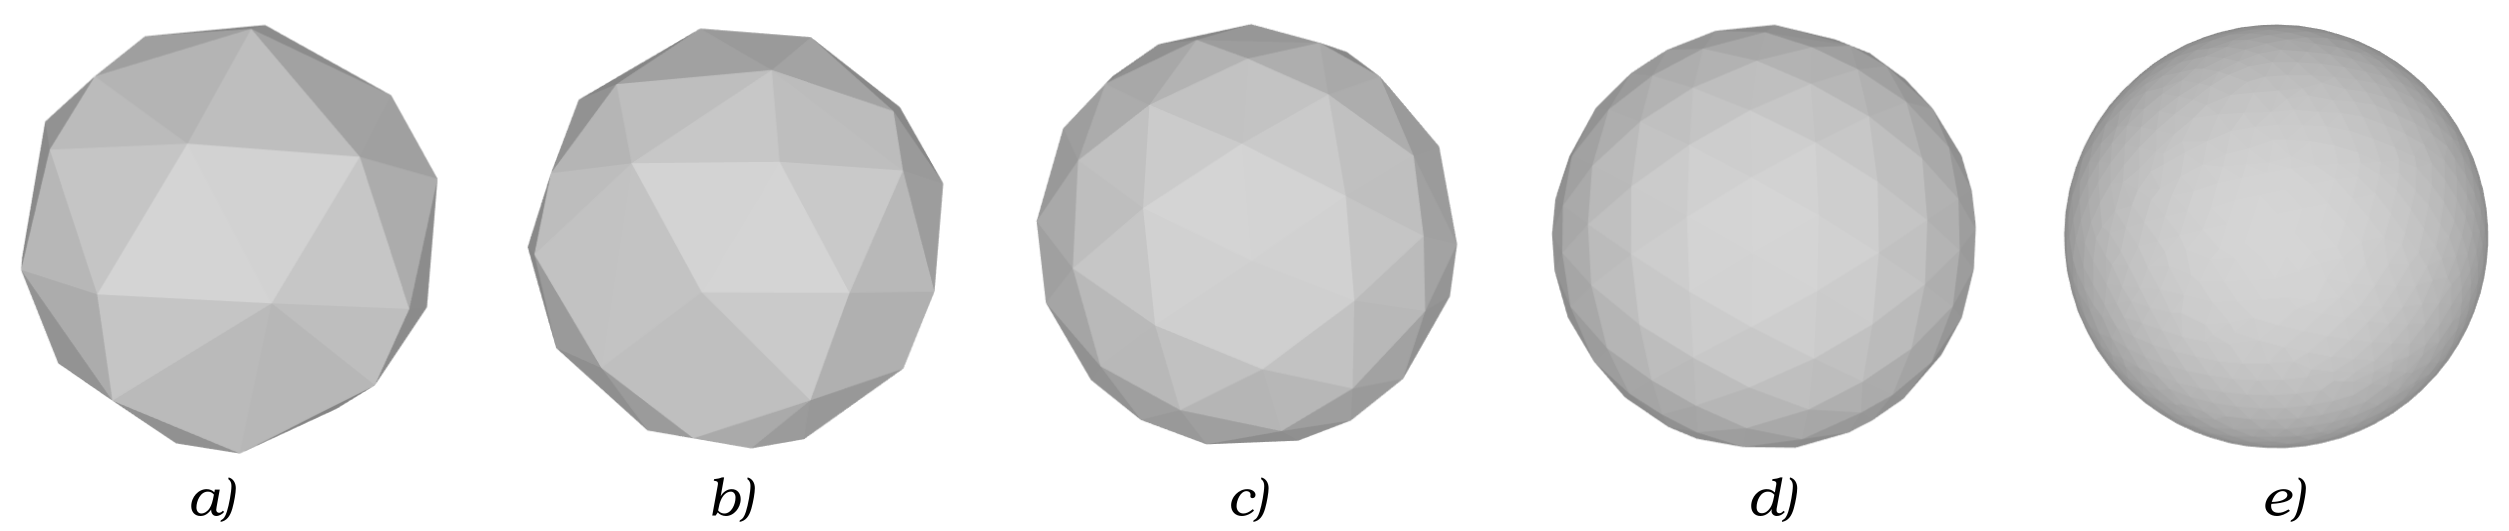
\includegraphics[width=1\textwidth]{images/sphere}}
        \caption[Triangulácia sféry]{Triangulácia sféry.}
        %id obrazku, pomocou ktoreho sa budeme na obrazok odvolavat
        \label{obr:sphere}
    \end{figure}

    Výsledky merania kritérií kvality môžeme vidieť v tabuľke \ref{tab:sphere}.
    
    \renewcommand*{\MinNumbera}{0.725}%
    \renewcommand*{\MaxNumbera}{0.954}%
    \pgfmathsetmacro{\MidNumberA}{(\MinNumberA+\MaxNumberA)/2}%
    \renewcommand*{\MinNumberB}{0.015}%
    \renewcommand*{\MaxNumberB}{0.085}%
    \pgfmathsetmacro{\MidNumberB}{(\MinNumberB+\MaxNumberB)/2}%
    \renewcommand*{\MinNumberC}{1.210}%
    \renewcommand*{\MaxNumberC}{1.305}%
    \pgfmathsetmacro{\MidNumberC}{(\MinNumberC+\MaxNumberC)/2}%
    \renewcommand*{\MinNumberD}{0.028}%
    \renewcommand*{\MaxNumberD}{0.136}%
    \pgfmathsetmacro{\MidNumberD}{(\MinNumberD+\MaxNumberD)/2}%
    \renewcommand*{\MinNumberE}{0.0}%
    \renewcommand*{\MaxNumberE}{5.140}%
    \pgfmathsetmacro{\MidNumberE}{(\MinNumberE+\MaxNumberE)/2}%
    \renewcommand*{\MinNumberF}{0.120}%
    \renewcommand*{\MaxNumberF}{0.646}%
    \pgfmathsetmacro{\MidNumberF}{(\MinNumberF+\MaxNumberF)/2}%
    \renewcommand*{\MinNumberG}{0.720}%
    \renewcommand*{\MaxNumberG}{0.951}%
    \pgfmathsetmacro{\MidNumberG}{(\MinNumberG+\MaxNumberG)/2}%
    \renewcommand*{\MinNumberH}{0.088}%
    \renewcommand*{\MaxNumberH}{0.112}%
    \pgfmathsetmacro{\MidNumberH}{(\MinNumberH+\MaxNumberH)/2}%


    \begin{table}[ht]
    \label{tab:sphere}
    \caption[Výsledky merania triangulácie sféry]{Výsledky merania}
        \begin{center}
            \begin{tabular}{| c |ABCDEFGH|}
                \hline
                \hline
                \multicolumn{9}{|c|}{Sféra} \\
                \hline
                \hline
                $\hspace{8mm} a \hspace{8mm}$ & $k_1$ & $k_2$ & $k_3$ & $k_4$ & $k_5$ & $k_6$ & $k_7$ & $k_8$ \EndTableHeader\\
                \hline
                \hline
                0.900 & 0.725 & 0.085 & 1.305 & 0.136 & 1.380 & 0.646 & 0.720 & 0.100 \\
                \hline
                0.700 & 0.798 & 0.079 & 1.321 & 0.131 & 0.000 & 0.617 & 0.792 & 0.112 \\
                \hline
                0.500 & 0.847 & 0.062 & 1.253 & 0.104 & 5.140 & 0.472 & 0.843 & 0.097 \\
                \hline
                0.300 & 0.895 & 0.041 & 1.274 & 0.074 & 0.005 & 0.291 & 0.892 & 0.103 \\
                \hline
                0.100 & 0.954 & 0.015 & 1.210 & 0.028 & 0.066 & 0.120 & 0.951 & 0.088 \\
                \hline
                \hline
            \end{tabular}
        \end{center}
    \end{table}

}

\newpage

\item{
    \textit{Elipsoid}
    \begin{equation}
    \label{eq:ellipsoid}
        \bigg ( \frac{x-1}{2} \bigg )^2 + \bigg (\frac{y-1}{3} \bigg )^2 + (z - 1)^2 - 1 = 0
    \end{equation}

    Na obrázku \ref{obr:ellipsoid} vidíme výslednú trianguláciu elipsoidu daného implicitnou 
    rovnicou \ref{eq:ellipsoid} s piatimi rôznymi dĺžkami strany $a$.
    \begin{enumerate}[a)]
    \item{
        $a=0.900$, $n=214$, $p=109$
    }
    \item{
        $a=0.700$, $n=332$, $p=168$
    }
    \item{
        $a=0.500$, $n=574$, $p=289$
    }
    \item{
        $a=0.300$, $n=1460$, $p=732$
    }
    \item{
        $a=0.150$, $n=5476$, $p=2740$
    }
    \end{enumerate}

    \begin{figure}
        \centerline{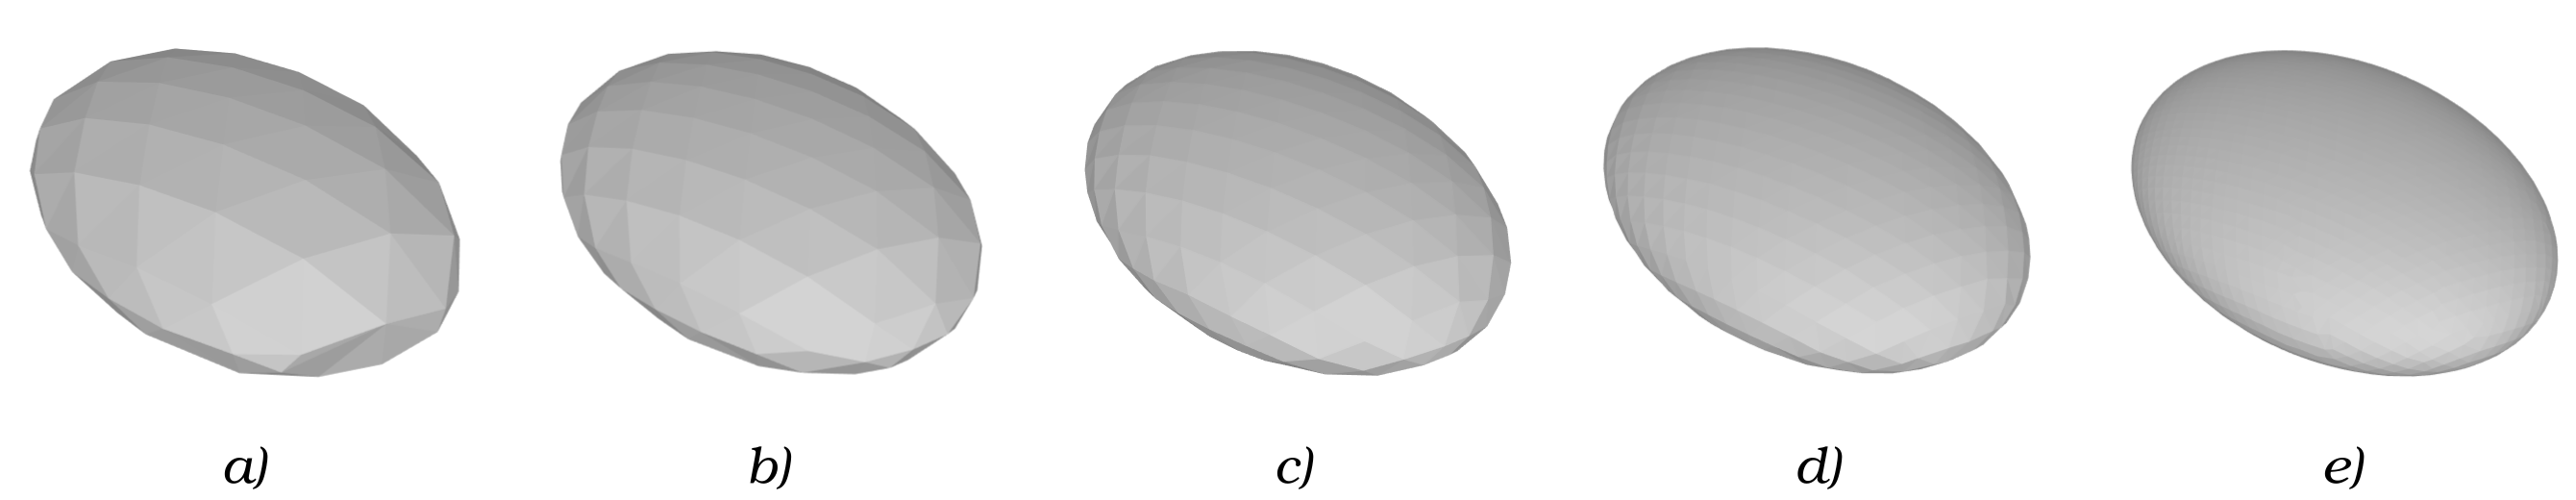
\includegraphics[width=1\textwidth]{images/ellipsoid}}
        \caption[Triangulácia elipsoidu]{Triangulácia elipsoidu.}
        %id obrazku, pomocou ktoreho sa budeme na obrazok odvolavat
        \label{obr:ellipsoid}
    \end{figure}

    Výsledky merania kritérií kvality môžeme vidieť v tabuľke \ref{tab:ellipsoid}.

    \renewcommand*{\MinNumberA}{0.802}%
    \renewcommand*{\MaxNumberA}{0.962}%
    \pgfmathsetmacro{\MidNumberA}{(\MinNumberA+\MaxNumberA)/2}%
    \renewcommand*{\MinNumberB}{0.013}%
    \renewcommand*{\MaxNumberB}{0.049}%
    \pgfmathsetmacro{\MidNumberB}{(\MinNumberB+\MaxNumberB)/2}%
    \renewcommand*{\MinNumberC}{1.142}%
    \renewcommand*{\MaxNumberC}{1.356}%
    \pgfmathsetmacro{\MidNumberC}{(\MinNumberC+\MaxNumberC)/2}%
    \renewcommand*{\MinNumberD}{0.057}%
    \renewcommand*{\MaxNumberD}{0.192}%
    \pgfmathsetmacro{\MidNumberD}{(\MinNumberD+\MaxNumberD)/2}%
    \renewcommand*{\MinNumberE}{0.0}%
    \renewcommand*{\MaxNumberE}{0.073}%
    \pgfmathsetmacro{\MidNumberE}{(\MinNumberE+\MaxNumberE)/2}%
    \renewcommand*{\MinNumberF}{0.338}%
    \renewcommand*{\MaxNumberF}{1.122}%
    \pgfmathsetmacro{\MidNumberF}{(\MinNumberF+\MaxNumberF)/2}%
    \renewcommand*{\MinNumberG}{0.796}%
    \renewcommand*{\MaxNumberG}{0.961}%
    \pgfmathsetmacro{\MidNumberG}{(\MinNumberG+\MaxNumberG)/2}%
    \renewcommand*{\MinNumberH}{0.061}%
    \renewcommand*{\MaxNumberH}{0.116}%
    \pgfmathsetmacro{\MidNumberH}{(\MinNumberH+\MaxNumberH)/2}%

    \begin{table}[ht]
    \label{tab:ellipsoid}
    \caption[Výsledky merania triangulácie elipsoidu]{Výsledky merania}
        \begin{center}
            \begin{tabular}{|c|A B C D E F G H|}
                \hline
                \hline
                \multicolumn{9}{|c|}{Elipsoid} \\
                \hline
                \hline
                $\hspace{8mm} a \hspace{8mm}$ & $k_1$ & $k_2$ & $k_3$ & $k_4$ & $k_5$ & $k_6$ & $k_7$ & $k_8$ \EndTableHeader\\
                \hline
                \hline
                0.900 & 0.802 & 0.049 & 1.356 & 0.192 & 
                0.073 & 1.220 & 0.796 & 0.116 \\
                \hline
                0.700 & 0.828 & 0.041 & 1.271 & 0.084 & 
                0.017 & 0.888 & 0.823 & 0.098\\
                \hline
                0.500 & 0.881 & 0.035 & 1.204 & 0.084 & 
                0.039 & 0.745 & 0.881 & 0.083\\
                \hline
                0.300 & 0.928 & 0.024 & 1.169 & 0.093 & 
                0.003 & 0.597 & 0.928 & 0.067\\
                \hline
                0.150 & 0.962 & 0.013 & 1.142 & 0.057 & 
                0.000 & 0.338 & 0.961 & 0.061\\
                \hline
                \hline
            \end{tabular}
        \end{center}
    \end{table}
}


\newpage

\item{
    \textit{Zaoblená kocka}
    \begin{equation}
    \label{eq:cubed_sphere}
        x^4+y^4+z^4-1 = 0
    \end{equation}

    Na obrázku \ref{obr:cubed_sphere} vidíme výslednú trianguláciu zaoblenej kocky danej implicitnou 
    rovnicou \ref{eq:cubed_sphere} s piatimi rôznymi dĺžkami strany $a$.
    \begin{enumerate}[a)]
    \item{
        $a=2.000$, $n=30$, $p=17$
    }
    \item{
        $a=1.000$, $n=68$, $p=36$
    }
    \item{
        $a=0.500$, $n=216$, $p=110$
    }
    \item{
        $a=0.250$, $n=748$, $p=376$
    }
    \item{
        $a=0.150$, $n=2034$, $p=1018$
    }
    \end{enumerate}

    \begin{figure}
        \centerline{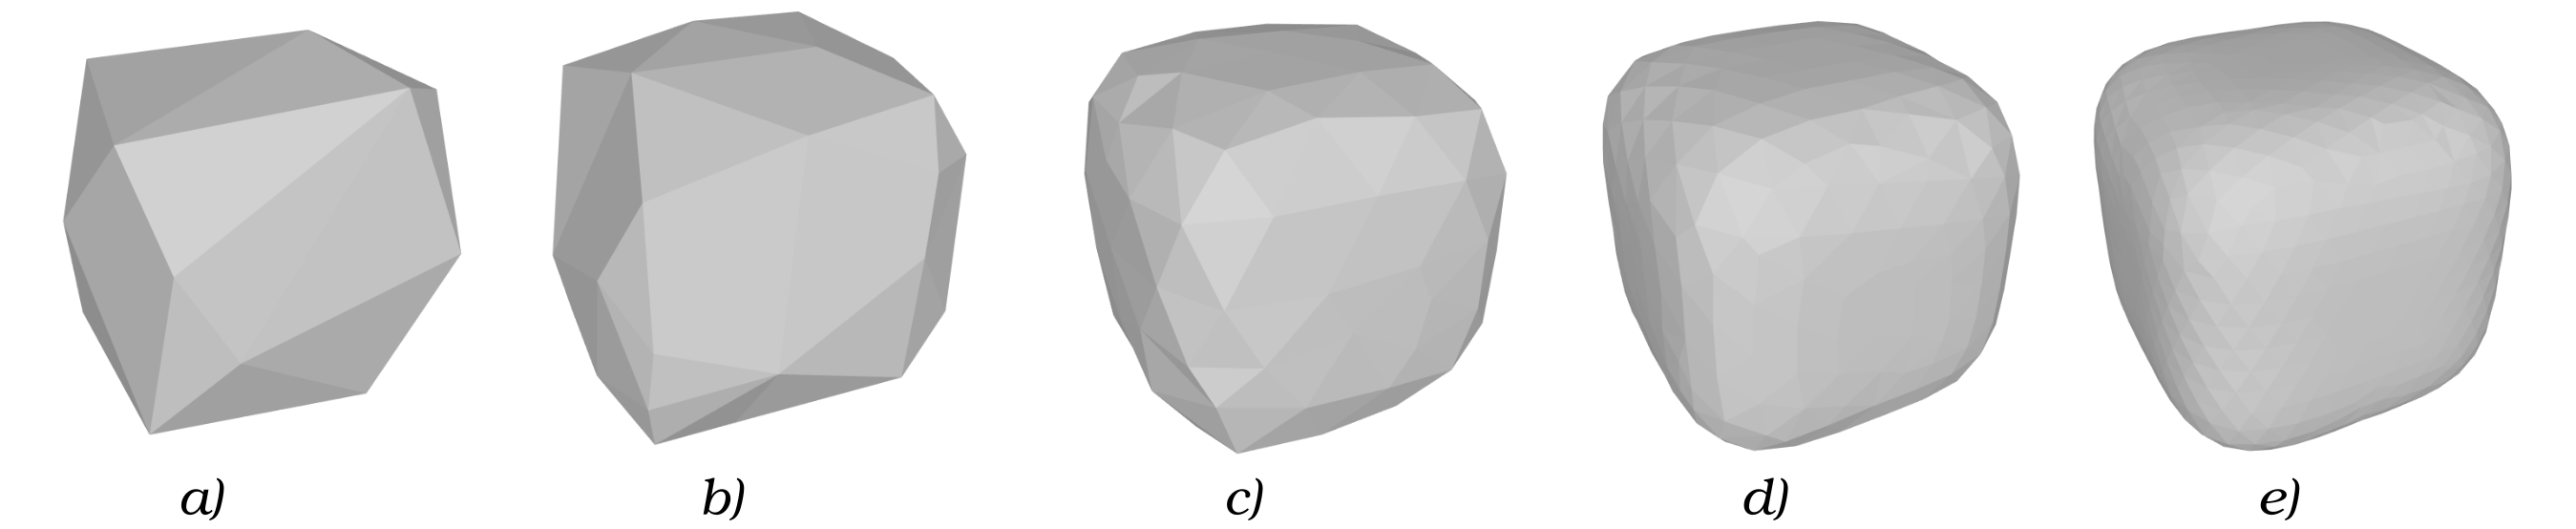
\includegraphics[width=1\textwidth]{images/cubed_sphere}}
        \caption[Triangulácia zaoblenej kocky]{Triangulácia zaoblenej kocky.}
        %id obrazku, pomocou ktoreho sa budeme na obrazok odvolavat
        \label{obr:cubed_sphere}
    \end{figure}

    Výsledky merania kritérií kvality môžeme vidieť v tabuľke \ref{tab:cubed_sphere}.

    \renewcommand*{\MinNumberA}{0.555}%
    \renewcommand*{\MaxNumberA}{0.949}%
    \pgfmathsetmacro{\MidNumberA}{(\MinNumberA+\MaxNumberA)/2}%
    \renewcommand*{\MinNumberB}{0.020}%
    \renewcommand*{\MaxNumberB}{0.077}%
    \pgfmathsetmacro{\MidNumberB}{(\MinNumberB+\MaxNumberB)/2}%
    \renewcommand*{\MinNumberC}{1.189}%
    \renewcommand*{\MaxNumberC}{1.681}%
    \pgfmathsetmacro{\MidNumberC}{(\MinNumberC+\MaxNumberC)/2}%
    \renewcommand*{\MinNumberD}{0.069}%
    \renewcommand*{\MaxNumberD}{0.244}%
    \pgfmathsetmacro{\MidNumberD}{(\MinNumberD+\MaxNumberD)/2}%
    \renewcommand*{\MinNumberE}{0.004}%
    \renewcommand*{\MaxNumberE}{0.524}%
    \pgfmathsetmacro{\MidNumberE}{(\MinNumberE+\MaxNumberE)/2}%
    \renewcommand*{\MinNumberF}{0.348}%
    \renewcommand*{\MaxNumberF}{1.128}%
    \pgfmathsetmacro{\MidNumberF}{(\MinNumberF+\MaxNumberF)/2}%
    \renewcommand*{\MinNumberG}{0.548}%
    \renewcommand*{\MaxNumberG}{0.947}%
    \pgfmathsetmacro{\MidNumberG}{(\MinNumberG+\MaxNumberG)/2}%
    \renewcommand*{\MinNumberH}{0.079}%
    \renewcommand*{\MaxNumberH}{0.152}%
    \pgfmathsetmacro{\MidNumberH}{(\MinNumberH+\MaxNumberH)/2}%
    
     \begin{table}[ht]
     \label{tab:cubed_sphere}
     \caption[Výsledky merania triangulácie zaoblenej kocky]{Výsledky merania}
        \begin{center}
            \begin{tabular}{|c|A B C D E F G H|}
                \hline
                \hline
                \multicolumn{9}{|c|}{Zaoblená kocka} \\
                \hline
                \hline
                $\hspace{8mm} a \hspace{8mm}$ & $k_1$ & $k_2$ & $k_3$ & $k_4$ & $k_5$ & $k_6$ & $k_7$ & $k_8$ \EndTableHeader\\
                \hline
                \hline
                2.000 & 0.555 & 0.066 & 1.681 & 0.143 & 0.482 & 1.228 & 0.548 & 0.136\\
                \hline
                1.000 & 0.750 & 0.077 & 1.454 & 0.244 & 0.524 & 1.062 & 0.738 & 0.152\\
                \hline
                0.500 & 0.865 & 0.051 & 1.286 & 0.173 & 0.040 & 0.837 & 0.861 & 0.111\\
                \hline
                0.250 & 0.935 & 0.031 & 1.189 & 0.099 & 0.026 & 0.591 & 0.932 & 0.080\\
                \hline
                0.150 & 0.949 & 0.020 & 1.189 & 0.069 & 0.004 & 0.348 & 0.947 & 0.079\\
                \hline
                \hline
            \end{tabular}
        \end{center}
    \end{table}
}

\newpage

\item{
    \textit{Torus}
    \begin{equation}
    \label{eq:torus}
        (x^2+y^2+z^2+1375)^2-6400(x^2+y^2) = 0
    \end{equation}

    Na obrázku \ref{obr:torus} vidíme výslednú trianguláciu torusu daného implicitnou 
    rovnicou \ref{eq:torus} s piatimi rôznymi dĺžkami strany $a$.
    \begin{enumerate}[a)]
    \item{
        $a=15$, $n=334$, $p=167$
    }
    \item{
        $a=12$, $n=494$, $p=247$
    }
    \item{
        $a=9$, $n=818$, $p=409$
    }
    \item{
        $a=6$, $n=1720$, $p=860$
    }
    \item{
        $a=3$, $n=6596$, $p=3297$
    }
    \end{enumerate}

    \begin{figure}
        \centerline{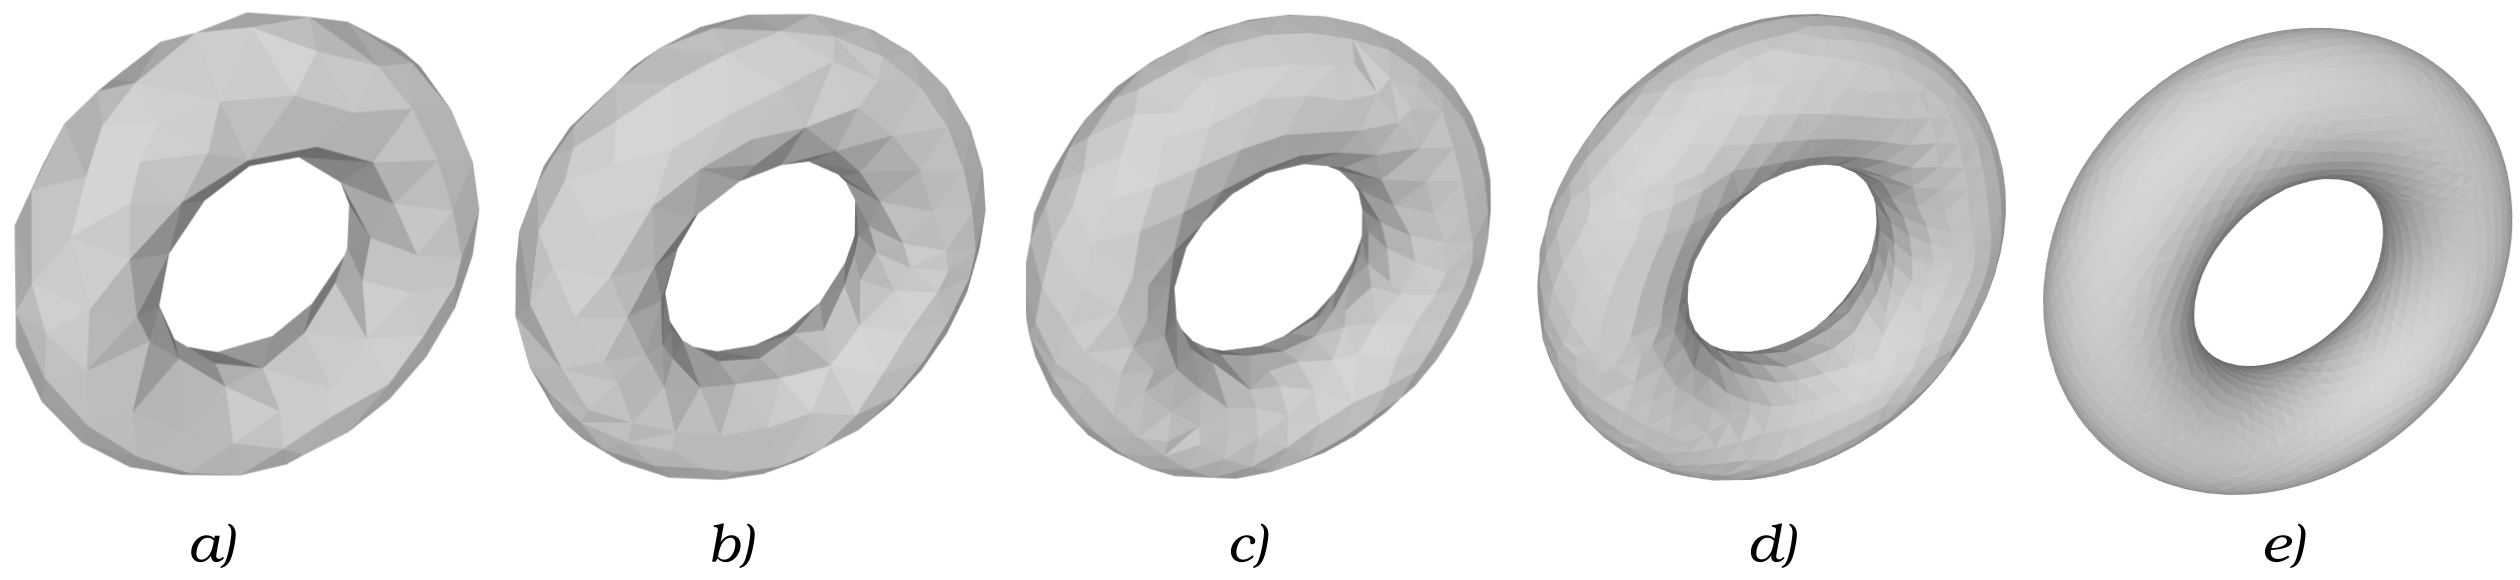
\includegraphics[width=1\textwidth]{images/torus}}
        \caption[Triangulácia torusu]{Triangulácia torusu.}
        %id obrazku, pomocou ktoreho sa budeme na obrazok odvolavat
        \label{obr:torus}
    \end{figure}

    Výsledky merania kritérií kvality môžeme vidieť v tabuľke \ref{tab:torus}.

     
    \renewcommand*{\MinNumberA}{0.856}%
    \renewcommand*{\MaxNumberA}{0.968}%
    \pgfmathsetmacro{\MidNumberA}{(\MinNumberA+\MaxNumberA)/2}%
    \renewcommand*{\MinNumberB}{0.016}%
    \renewcommand*{\MaxNumberB}{0.060}%
    \pgfmathsetmacro{\MidNumberB}{(\MinNumberB+\MaxNumberB)/2}%
    \renewcommand*{\MinNumberC}{1.197}%
    \renewcommand*{\MaxNumberC}{1.331}%
    \pgfmathsetmacro{\MidNumberC}{(\MinNumberC+\MaxNumberC)/2}%
    \renewcommand*{\MinNumberD}{0.052}%
    \renewcommand*{\MaxNumberD}{0.188}%
    \pgfmathsetmacro{\MidNumberD}{(\MinNumberD+\MaxNumberD)/2}%
    \renewcommand*{\MinNumberE}{0.000}%
    \renewcommand*{\MaxNumberE}{0.067}%
    \pgfmathsetmacro{\MidNumberE}{(\MinNumberE+\MaxNumberE)/2}%
    \renewcommand*{\MinNumberF}{0.467}%
    \renewcommand*{\MaxNumberF}{0.974}%
    \pgfmathsetmacro{\MidNumberF}{(\MinNumberF+\MaxNumberF)/2}%
    \renewcommand*{\MinNumberG}{0.851}%
    \renewcommand*{\MaxNumberG}{0.966}%
    \pgfmathsetmacro{\MidNumberG}{(\MinNumberG+\MaxNumberG)/2}%
    \renewcommand*{\MinNumberH}{0.083}%
    \renewcommand*{\MaxNumberH}{0.117}%
    \pgfmathsetmacro{\MidNumberH}{(\MinNumberH+\MaxNumberH)/2}%

  
     \begin{table}[ht]
     \label{tab:torus}
     \caption[Výsledky merania triangulácie torusu]{Výsledky merania}
        \begin{center}
            \begin{tabular}{|c|A B C D E F G H|}
                \hline
                \hline
                \multicolumn{9}{|c|}{Torus} \\
                \hline
                \hline
                $\hspace{5mm} a \hspace{5mm}$ & $k_1$ & $k_2$ & $k_3$ & $k_4$ & $k_5$ & $k_6$ & $k_7$ & $k_8$ \EndTableHeader\\
                \hline
                \hline
                15 & 0.856 & 0.060 & 1.324 & 0.188 & 0.000 & 0.974 & 0.851 & 0.116\\
                \hline
                12 & 0.882 & 0.051 & 1.331 & 0.151 & 0.067 & 0.823 & 0.878 & 0.117\\
                \hline
                9 & 0.916 & 0.042 & 1.284 & 0.097 & 0.013 & 0.671 & 0.912 & 0.109\\
                \hline
                6 & 0.946 & 0.030 & 1.227 & 0.078 & 0.001 & 0.467 & 0.944 & 0.094\\
                \hline
                3 & 0.968 & 0.016 & 1.197 & 0.052 & 0.002 & 0.868 & 0.966 & 0.083\\
                \hline
                \hline
            \end{tabular}
        \end{center}
    \end{table}

}

\newpage

\item{
    \textit{Genus}
    \begin{equation}
    \label{eq:genus}
        2y(y^2-3x^2)(1-z^2)+(x^2+y^2)^2-(9z^2-1)(1-z^2) = 0
    \end{equation}

    Na obrázku \ref{obr:genus} vidíme výslednú trianguláciu torusu daného implicitnou 
    rovnicou \ref{eq:genus} s piatimi rôznymi dĺžkami strany $a$.
    \begin{enumerate}[a)]
    \item{
        $a=0.225$, $n=1566$, $p=781$
    }
    \item{
        $a=0.200$, $n=1958$, $p=977$
    }
    \item{
        $a=0.175$, $n=2480$, $p=1238$
    }
    \item{
        $a=0.150$, $n=3330$, $p=1663$
    }
    \item{
        $a=0.125$, $n=4614$, $p=2305$
    }
    \end{enumerate}

    \begin{figure}
        \centerline{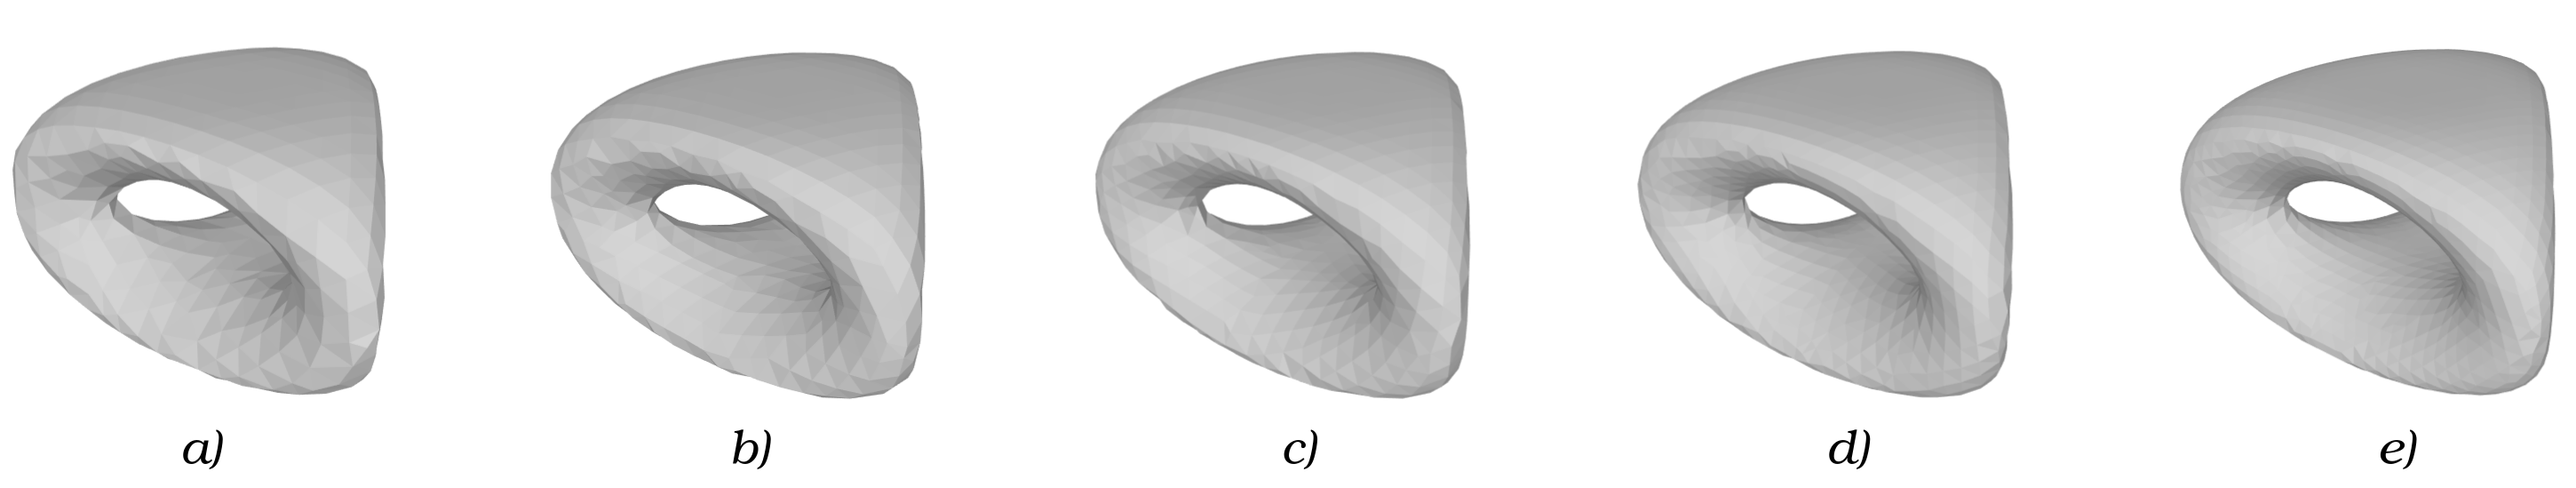
\includegraphics[width=1\textwidth]{images/genus}}
        \caption[Triangulácia genusu]{Triangulácia genusu.}
        %id obrazku, pomocou ktoreho sa budeme na obrazok odvolavat
        \label{obr:genus}
    \end{figure}

    Výsledky merania kritérií kvality môžeme vidieť v tabuľke \ref{tab:genus}.

    \renewcommand*{\MinNumberA}{0.912}%
    \renewcommand*{\MaxNumberA}{0.954}%
    \pgfmathsetmacro{\MidNumberA}{(\MinNumberA+\MaxNumberA)/2}%
    \renewcommand*{\MinNumberB}{0.018}%
    \renewcommand*{\MaxNumberB}{0.029}%
    \pgfmathsetmacro{\MidNumberB}{(\MinNumberB+\MaxNumberB)/2}%
    \renewcommand*{\MinNumberC}{1.223}%
    \renewcommand*{\MaxNumberC}{1.303}%
    \pgfmathsetmacro{\MidNumberC}{(\MinNumberC+\MaxNumberC)/2}%
    \renewcommand*{\MinNumberD}{0.099}%
    \renewcommand*{\MaxNumberD}{0.307}%
    \pgfmathsetmacro{\MidNumberD}{(\MinNumberD+\MaxNumberD)/2}%
    \renewcommand*{\MinNumberE}{0.001}%
    \renewcommand*{\MaxNumberE}{0.005}%
    \pgfmathsetmacro{\MidNumberE}{(\MinNumberE+\MaxNumberE)/2}%
    \renewcommand*{\MinNumberF}{0.896}%
    \renewcommand*{\MaxNumberF}{2.716}%
    \pgfmathsetmacro{\MidNumberF}{(\MinNumberF+\MaxNumberF)/2}%
    \renewcommand*{\MinNumberG}{0.907}%
    \renewcommand*{\MaxNumberG}{0.951}%
    \pgfmathsetmacro{\MidNumberG}{(\MinNumberG+\MaxNumberG)/2}%
    \renewcommand*{\MinNumberH}{0.092}%
    \renewcommand*{\MaxNumberH}{0.114}%
    \pgfmathsetmacro{\MidNumberH}{(\MinNumberH+\MaxNumberH)/2}%

    \begin{table}[ht]
     \label{tab:genus}
     \caption[Výsledky merania triangulácie genusu]{Výsledky merania}
        \begin{center}
            \begin{tabular}{|c|A B C D E F G H|}
                \hline
                \hline
                \multicolumn{9}{|c|}{Genus} \\
                \hline
                \hline
                $\hspace{8mm} a \hspace{8mm}$ & $k_1$ & $k_2$ & $k_3$ & $k_4$ & $k_5$ & $k_6$ & $k_7$ & $k_8$ \EndTableHeader\\
                \hline
                \hline
                0.225 & 0.912 & 0.029 & 1.301 & 0.153 & 0.005 & 1.405 & 0.907 & 0.114\\
                \hline
                0.200 & 0.918 & 0.027 & 1.303 & 0.307 & 0.001 & 2.716 & 0.913 & 0.112\\
                \hline
                0.175 & 0.931 & 0.024 & 1.262 & 0.203 & 0.002 & 1.141 & 0.927 & 0.103\\
                \hline
                0.150 & 0.937 & 0.021 & 1.266 & 0.185 & 0.001 & 0.968 & 0.933 & 0.104\\
                \hline
                0.125 & 0.954 & 0.018 & 1.223 & 0.099 & 0.001 & 0.896 & 0.951 & 0.092\\
                \hline
                \hline
            \end{tabular}
        \end{center}
    \end{table}

}
\newpage

\item{
    \textit{Tetrahedron}
    \begin{equation}
    \label{eq:tetrahedron}
        x^4+2x^2y^2+2x^2z^2+y^4+2y^2z^2+z^4+8xyz-10x^2-10y^2-10z^2+20 = 0
    \end{equation}

    Na obrázku \ref{obr:tetrahedron} vidíme výslednú trianguláciu tetrahedronu daného implicitnou 
    rovnicou \ref{eq:tetrahedron} s piatimi rôznymi dĺžkami strany $a$.
    \begin{enumerate}[a)]
    \item{
        $a=0.600$, $n=1132$, $p=562$
    }
    \item{
        $a=0.500$, $n=1562$, $p=777$
    }
    \item{
        $a=0.400$, $n=2366$, $p=1179$
    }
    \item{
        $a=0.300$, $n=4002$, $p=1996$
    }
    \item{
        $a=0.200$, $n=8476$, $p=4234$
    }
    \end{enumerate}

    \begin{figure}
        \centerline{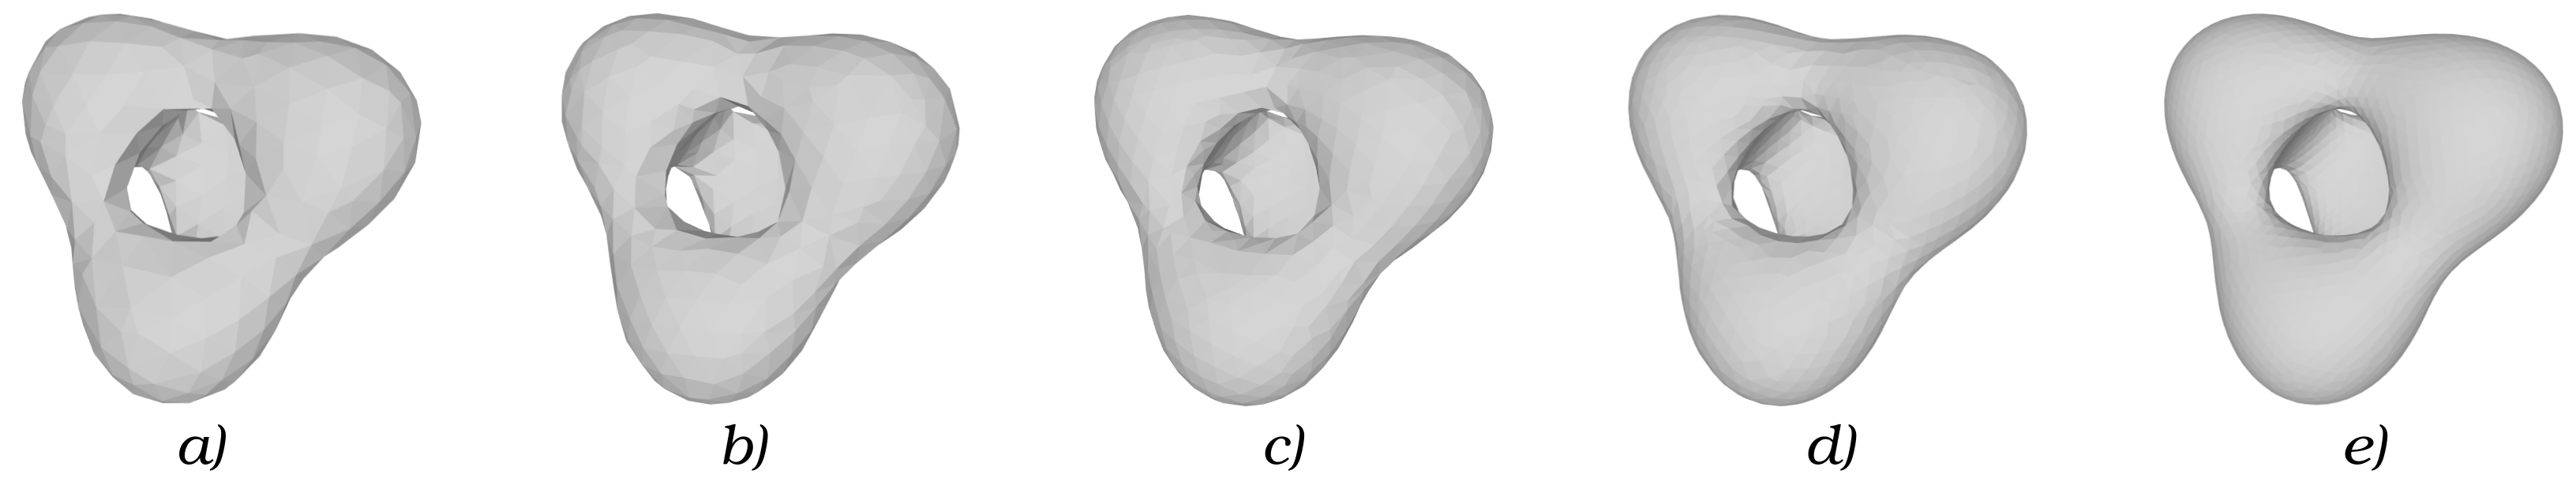
\includegraphics[width=1\textwidth]{images/tetrahedron}}
        \caption[Triangulácia tetrahedronu]{Triangulácia tetrahedronu.}
        %id obrazku, pomocou ktoreho sa budeme na obrazok odvolavat
        \label{obr:tetrahedron}
    \end{figure}

    Výsledky merania kritérií kvality môžeme vidieť v tabuľke \ref{tab:tetrahedron}.

    
    \renewcommand*{\MinNumberA}{0.885}%
    \renewcommand*{\MaxNumberA}{0.966}%
    \pgfmathsetmacro{\MidNumberA}{(\MinNumberA+\MaxNumberA)/2}%
    \renewcommand*{\MinNumberB}{0.015}%
    \renewcommand*{\MaxNumberB}{0.040}%
    \pgfmathsetmacro{\MidNumberB}{(\MinNumberB+\MaxNumberB)/2}%
    \renewcommand*{\MinNumberC}{1.232}%
    \renewcommand*{\MaxNumberC}{1.358}%
    \pgfmathsetmacro{\MidNumberC}{(\MinNumberC+\MaxNumberC)/2}%
    \renewcommand*{\MinNumberD}{0.067}%
    \renewcommand*{\MaxNumberD}{0.441}%
    \pgfmathsetmacro{\MidNumberD}{(\MinNumberD+\MaxNumberD)/2}%
    \renewcommand*{\MinNumberE}{0.001}%
    \renewcommand*{\MaxNumberE}{0.059}%
    \pgfmathsetmacro{\MidNumberE}{(\MinNumberE+\MaxNumberE)/2}%
    \renewcommand*{\MinNumberF}{0.648}%
    \renewcommand*{\MaxNumberF}{2.903}%
    \pgfmathsetmacro{\MidNumberF}{(\MinNumberF+\MaxNumberF)/2}%
    \renewcommand*{\MinNumberG}{0.880}%
    \renewcommand*{\MaxNumberG}{0.963}%
    \pgfmathsetmacro{\MidNumberG}{(\MinNumberG+\MaxNumberG)/2}%
    \renewcommand*{\MinNumberH}{0.097}%
    \renewcommand*{\MaxNumberH}{0.129}%
    \pgfmathsetmacro{\MidNumberH}{(\MinNumberH+\MaxNumberH)/2}%


    \begin{table}[ht]
     \label{tab:tetrahedron}
     \caption[Výsledky merania triangulácie tetrahedronu]{Výsledky merania}
        \begin{center}
            \begin{tabular}{|c|A B C D E F G H|}
                \hline
                \multicolumn{9}{|c|}{Tetrahedron} \\
                \hline
                $\hspace{8mm} a \hspace{8mm}$ & $k_1$ & $k_2$ & $k_3$ & $k_4$ & $k_5$ & $k_6$ & $k_7$ & $k_8$ \EndTableHeader\\
                \hline
                0.600 & 0.885 & 0.040 & 1.358 & 0.167 & 0.059 & 1.837 & 0.880 & 0.129\\
                \hline
                0.500 & 0.903 & 0.034 & 1.314 & 0.441 & 0.021 & 2.903 & 0.898 & 0.121\\
                \hline
                0.400 & 0.917 & 0.028 & 1.306 & 0.128 & 0.005 & 1.258 & 0.913 & 0.118\\
                \hline
                0.300 & 0.940 & 0.022 & 1.274 & 0.118 & 0.009 & 0.984 & 0.936 & 0.109\\
                \hline
                0.200 & 0.966 & 0.015 & 1.232 & 0.067 & 0.001 & 0.648 & 0.963 & 0.097\\
                \hline
                \hline
            \end{tabular}
        \end{center}
    \end{table}

}
\newpage
\item{
    \textit{Plocha konštantného súčinu vzdialeností od štvorice bodov}
    \begin{equation}
    \label{eq:blobby}
        a \cdot b \cdot c \cdot d -1.1 = 0
    \end{equation}
    pričom

    $a = \sqrt{(x-1)^2+y^2+z^2}$,

    $b=\sqrt{(x+1)^2+y^2+z^2}$,
    
    $c=\sqrt{x^2+(y-1)^2+z^2}$,
        
    $d=\sqrt{x^2+(y+1)^2+z^2}$.

    Na obrázku \ref{obr:blobby} vidíme výslednú trianguláciu plochy danej implicitnou 
    rovnicou \ref{eq:blobby} s piatimi rôznymi dĺžkami strany $a$.
    \begin{enumerate}[a)]
    \item{
        $a=0.200$, $n=542$, $p=273$
    }
    \item{
        $a=0.150$, $n=922$, $p=463$
    }
    \item{
        $a=0.120$, $n=1340$, $p=672$
    }
    \item{
        $a=0.100$, $n=1902$, $p=953$
    }
    \item{
        $a=0.070$, $n=3728$, $p=1866$
    }
    \end{enumerate}

    \begin{figure}
        \centerline{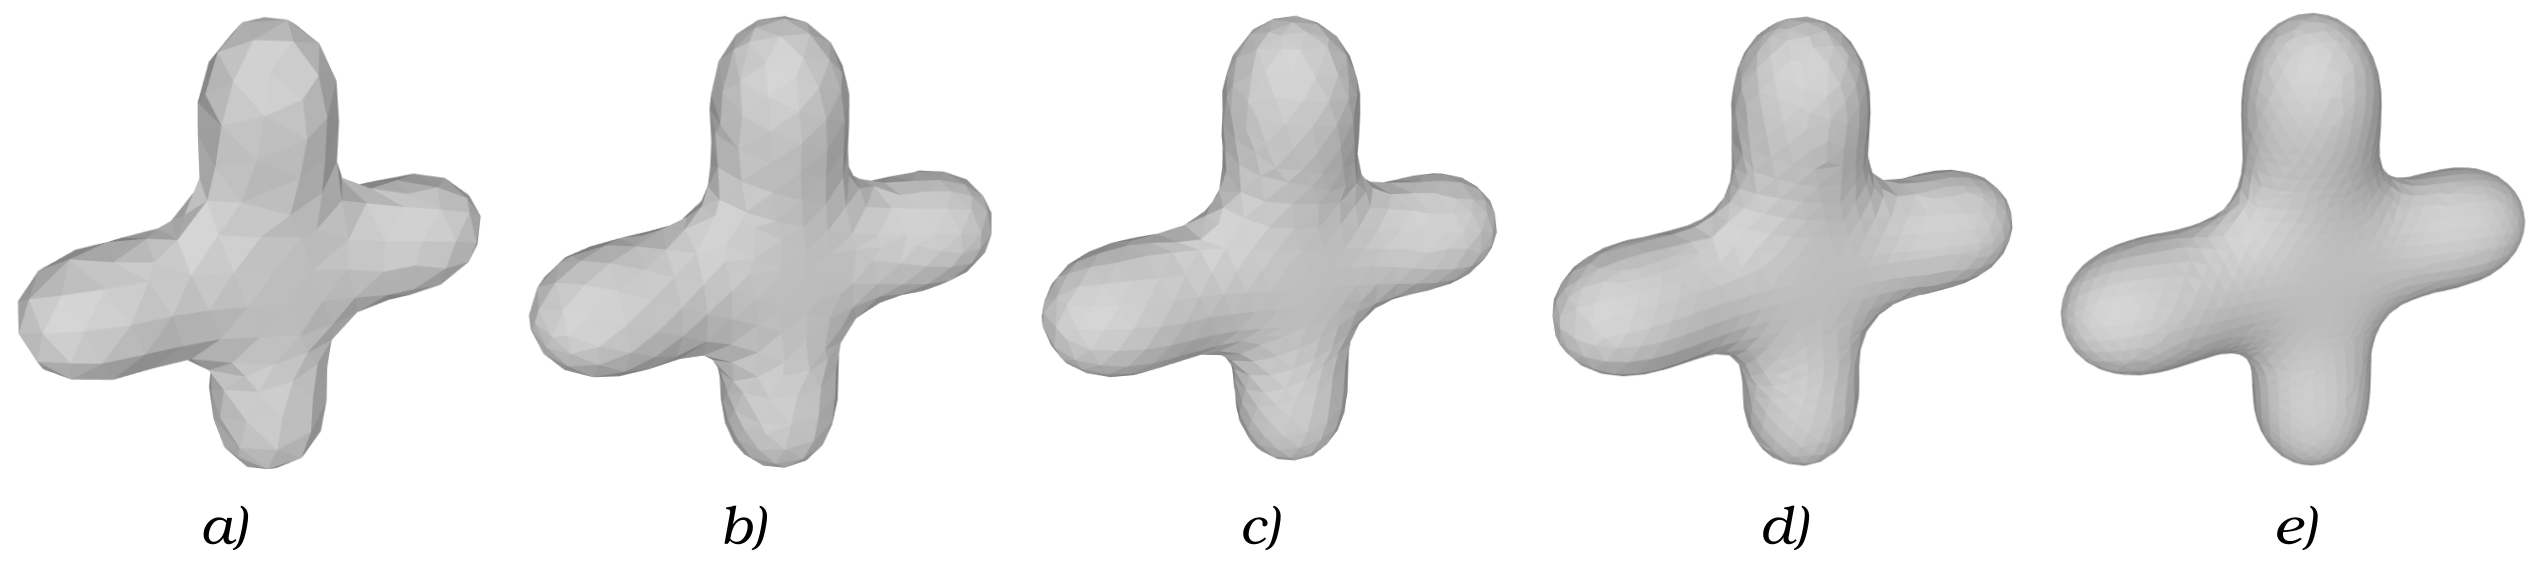
\includegraphics[width=1\textwidth]{images/blobby}}
        \caption[Plocha konštantného súčinu vzdialeností od štvorice bodov]
        {Plocha konštantného súčinu vzdialeností od štvorice bodov.}
        %id obrazku, pomocou ktoreho sa budeme na obrazok odvolavat
        \label{obr:blobby}
    \end{figure}

    Výsledky merania kritérií kvality môžeme vidieť v tabuľke \ref{tab:blobby}.
    
    \renewcommand*{\MinNumberA}{0.881}%
    \renewcommand*{\MaxNumberA}{0.962}%
    \pgfmathsetmacro{\MidNumberA}{(\MinNumberA+\MaxNumberA)/2}%
    \renewcommand*{\MinNumberB}{0.021}%
    \renewcommand*{\MaxNumberB}{0.051}%
    \pgfmathsetmacro{\MidNumberB}{(\MinNumberB+\MaxNumberB)/2}%
    \renewcommand*{\MinNumberC}{1.216}%
    \renewcommand*{\MaxNumberC}{1.335}%
    \pgfmathsetmacro{\MidNumberC}{(\MinNumberC+\MaxNumberC)/2}%
    \renewcommand*{\MinNumberD}{0.071}%
    \renewcommand*{\MaxNumberD}{0.183}%
    \pgfmathsetmacro{\MidNumberD}{(\MinNumberD+\MaxNumberD)/2}%
    \renewcommand*{\MinNumberE}{0.003}%
    \renewcommand*{\MaxNumberE}{0.163}%
    \pgfmathsetmacro{\MidNumberE}{(\MinNumberE+\MaxNumberE)/2}%
    \renewcommand*{\MinNumberF}{0.520}%
    \renewcommand*{\MaxNumberF}{1.208}%
    \pgfmathsetmacro{\MidNumberF}{(\MinNumberF+\MaxNumberF)/2}%
    \renewcommand*{\MinNumberG}{0.876}%
    \renewcommand*{\MaxNumberG}{0.960}%
    \pgfmathsetmacro{\MidNumberG}{(\MinNumberG+\MaxNumberG)/2}%
    \renewcommand*{\MinNumberH}{0.092}%
    \renewcommand*{\MaxNumberH}{0.119}%
    \pgfmathsetmacro{\MidNumberH}{(\MinNumberH+\MaxNumberH)/2}%


    \begin{table}[ht]
     \label{tab:blobby}
     \caption[Výsledky merania triangulácie plochy konštantného súčinu vzdialeností od štvorice bodov]{Výsledky merania}
        \begin{center}
            \begin{tabular}{|c|A B C D E F G H|}
                \hline
                \multicolumn{9}{|c|}{Plocha konštantného súčinu vzdialeností od štvorice bodov} \\
                \hline
                $\hspace{8mm} a \hspace{8mm}$ & $k_1$ & $k_2$ & $k_3$ & $k_4$ & $k_5$ & $k_6$ & $k_7$ & $k_8$ \EndTableHeader\\
                \hline
                0.200 & 0.881 & 0.051 & 1.335 & 0.183 & 0.005 & 1.208 & 0.876 & 0.119\\
                \hline
                0.150 & 0.901 & 0.039 & 1.278 & 0.127 & 0.163 & 0.899 & 0.898 & 0.108\\
                \hline
                0.120 & 0.935 & 0.034 & 1.264 & 0.114 & 0.011 & 0.831 & 0.932 & 0.106\\
                \hline
                0.100 & 0.943 & 0.028 & 1.259 & 0.089 & 0.003 & 0.761 & 0.940 & 0.104\\
                \hline
                0.070 & 0.962 & 0.021 & 1.216 & 0.071 & 0.003 & 0.520 & 0.960 & 0.092\\
                \hline
                \hline
            \end{tabular}
        \end{center}
    \end{table}

}

\newpage
\item{
    \textit{Plocha \textit{tanglecube}}
    \begin{equation}
    \label{eq:joined_spheres}
        x^4-5x^2+y^4-5y^2+z^4-5z^2+11.8 = 0
    \end{equation}

    Na obrázku \ref{obr:joined_spheres} vidíme výslednú trianguláciu plochy \textit{tanglecube} 
    danej implicitnou rovnicou \ref{eq:joined_spheres} s piatimi rôznymi dĺžkami strany $a$.
    \begin{enumerate}[a)]
    \item{
        $a=0.300$, $n=3192$, $p=1588$
    }
    \item{
        $a=0.275$, $n=3768$, $p=1876$
    }
    \item{
        $a=0.250$, $n=4464$, $p=2224$
    }
    \item{
        $a=0.200$, $n=6680$, $p=3332$
    }
    \item{
        $a=0.150$, $n=11466$, $p=5742$
    }
    \end{enumerate}

    \begin{figure}
        \centerline{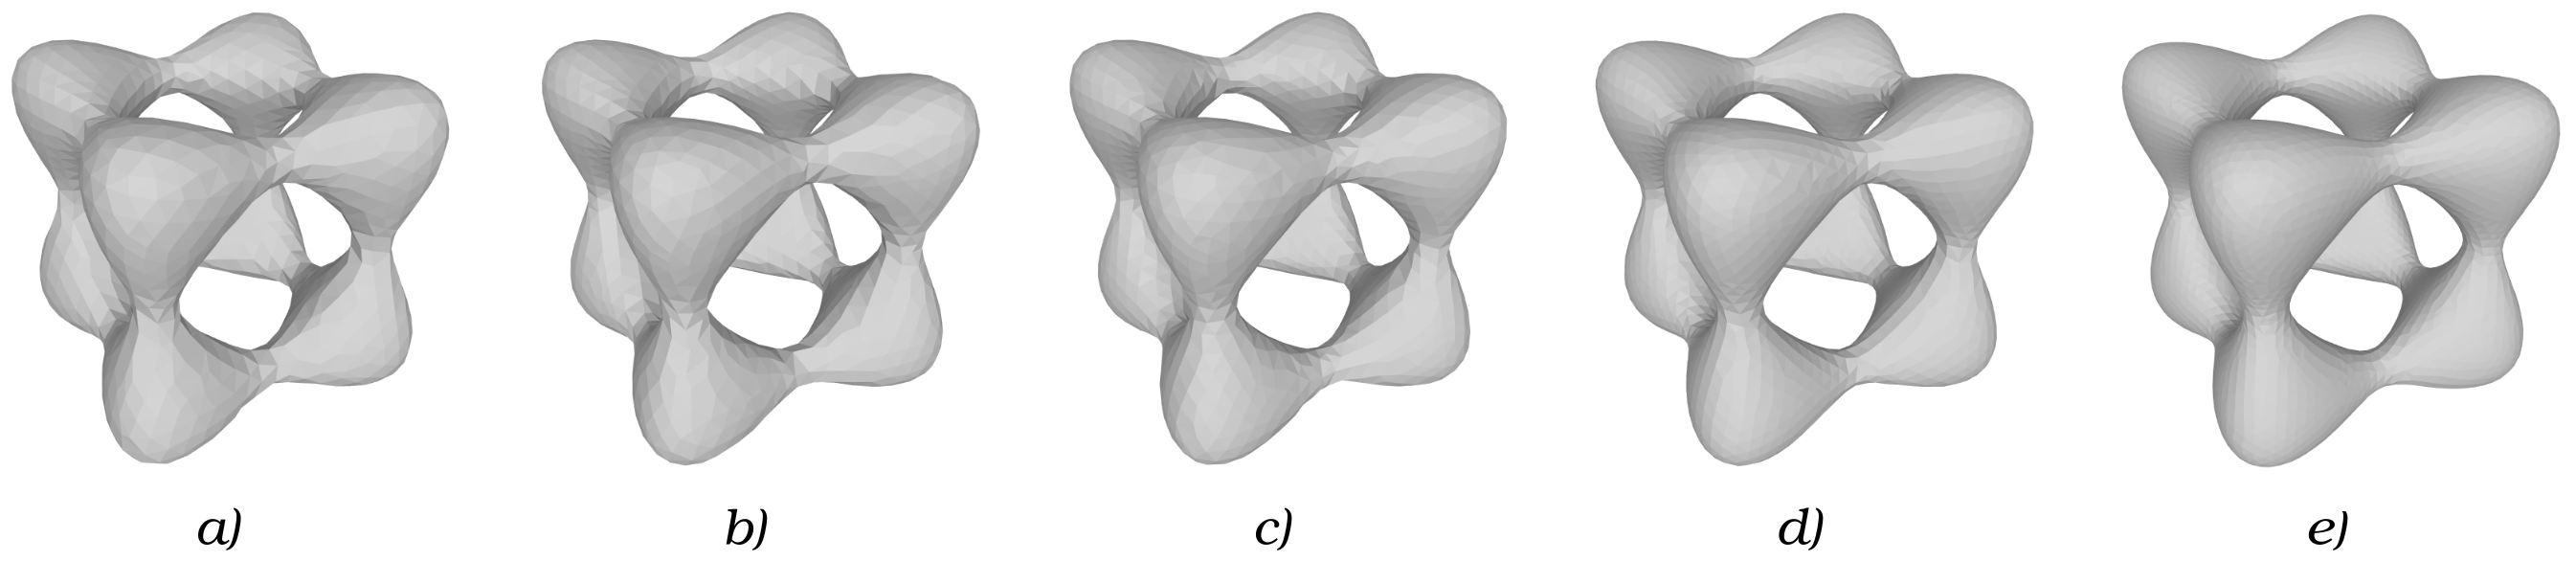
\includegraphics[width=1\textwidth]{images/joined_spheres}}
        \caption[Triangulácia plochy \textit{tanglecube}]{Triangulácia plochy \textit{tanglecube}.}
        %id obrazku, pomocou ktoreho sa budeme na obrazok odvolavat
        \label{obr:joined_spheres}
    \end{figure}

    Výsledky merania kritérií kvality môžeme vidieť v tabuľke \ref{tab:joined_spheres}.


    \renewcommand*{\MinNumberA}{0.911}%
    \renewcommand*{\MaxNumberA}{0.960}%
    \pgfmathsetmacro{\MidNumberA}{(\MinNumberA+\MaxNumberA)/2}%
    \renewcommand*{\MinNumberB}{0.020}%
    \renewcommand*{\MaxNumberB}{0.036}%
    \pgfmathsetmacro{\MidNumberB}{(\MinNumberB+\MaxNumberB)/2}%
    \renewcommand*{\MinNumberC}{1.239}%
    \renewcommand*{\MaxNumberC}{1.304}%
    \pgfmathsetmacro{\MidNumberC}{(\MinNumberC+\MaxNumberC)/2}%
    \renewcommand*{\MinNumberD}{0.077}%
    \renewcommand*{\MaxNumberD}{0.141}%
    \pgfmathsetmacro{\MidNumberD}{(\MinNumberD+\MaxNumberD)/2}%
    \renewcommand*{\MinNumberE}{0.000}%
    \renewcommand*{\MaxNumberE}{0.010}%
    \pgfmathsetmacro{\MidNumberE}{(\MinNumberE+\MaxNumberE)/2}%
    \renewcommand*{\MinNumberF}{0.694}%
    \renewcommand*{\MaxNumberF}{1.192}%
    \pgfmathsetmacro{\MidNumberF}{(\MinNumberF+\MaxNumberF)/2}%
    \renewcommand*{\MinNumberG}{0.906}%
    \renewcommand*{\MaxNumberG}{0.957}%
    \pgfmathsetmacro{\MidNumberG}{(\MinNumberG+\MaxNumberG)/2}%
    \renewcommand*{\MinNumberH}{0.098}%
    \renewcommand*{\MaxNumberH}{0.115}%
    \pgfmathsetmacro{\MidNumberH}{(\MinNumberH+\MaxNumberH)/2}%



    \begin{table}[ht]
     \label{tab:joined_spheres}
     \caption[Výsledky merania triangulácie plochy\textit{tanglecube}]{Výsledky merania}
        \begin{center}
            \begin{tabular}{|c|A B C D E F G H|}
                \hline
                \multicolumn{9}{|c|}{Plocha \textit{tanglecube}} \\
                \hline
                $\hspace{8mm} a \hspace{8mm}$ & $k_1$ & $k_2$ & $k_3$ & $k_4$ & $k_5$ & $k_6$ & $k_7$ & $k_8$ \EndTableHeader\\
                \hline
                0.300 & 0.911 & 0.036 & 1.304 & 0.137 & 0.010 & 1.192 & 0.906 & 0.115\\
                \hline
                0.275 & 0.915 & 0.033 & 1.298 & 0.141 & 0.001 & 1.178 & 0.910 & 0.115\\
                \hline
                0.250 & 0.924 & 0.031 & 1.285 & 0.135 & 0.000 & 1.106 & 0.920 & 0.110\\
                \hline
                0.200 & 0.943 & 0.026 & 1.248 & 0.109 & 0.003 & 0.836 & 0.940 & 0.101\\
                \hline
                0.150 & 0.960 & 0.020 & 1.239 & 0.077 & 0.000 & 0.694 & 0.957 & 0.098\\
                \hline
                \hline
            \end{tabular}
        \end{center}
    \end{table}

}

\end{enumerate}
\newpage

\subsection{Orezávanie na ohraničujúcu obálku}

V kapitole \ref{kap:important_methods} sme opísali dva spôsoby orezávania na ohraničujúcu obálku.
Prvý spôsob orezávania je pripínanie na najbližší bod ohraničujúcej obálky, teda v smere normály 
niektorej zo stien tejto obálky. Druhý spôsob je v smere ťažnice trojuholníka. Oba spôsoby demonštrujeme obrázkami
a slovne popíšeme naše pozorovania.

Na obrázku \ref{obr:cut_sphere_normal} môžeme vidieť trianguláciu zrezanej sféry pre 4 rôzne dĺžky 
hrany $a$, kde je orezávanie docielené pripínaním na najbližší bod obálky. Vidíme, že na stenách obálky 
je triangulácia veľmi nepresná.

\begin{figure}
    \centerline{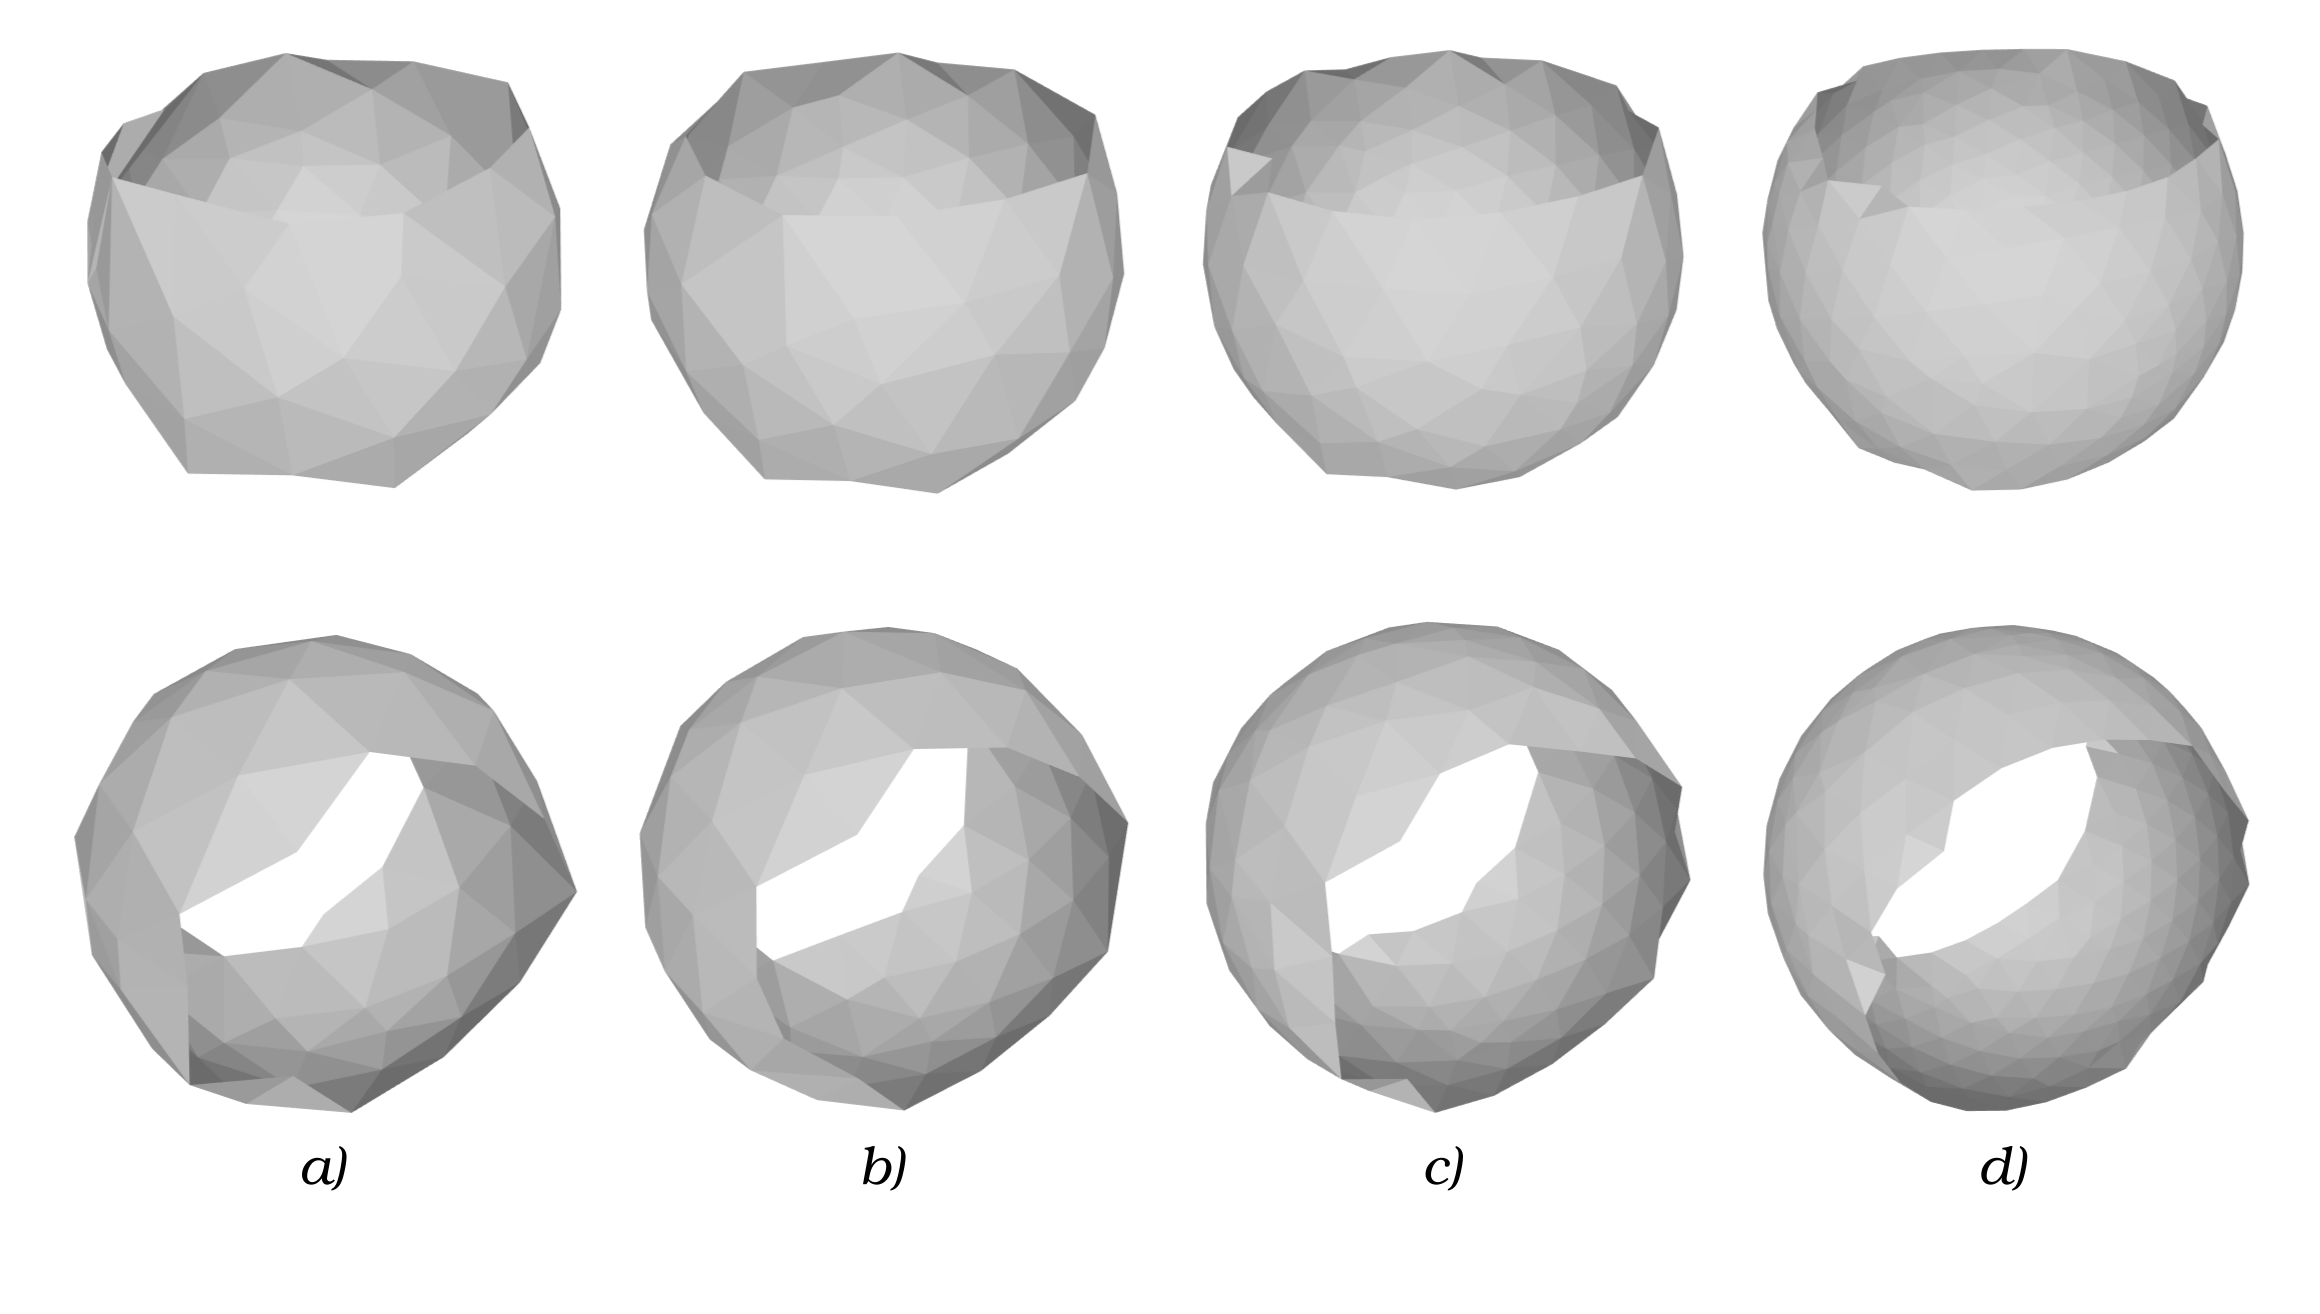
\includegraphics[width=0.8\textwidth]{images/cut_sphere_normal}}
    \caption[Ohraničená triangulácia gule -- premietanie na najbližší bod]
    {Premietanie na najbližší bod.}
    %id obrazku, pomocou ktoreho sa budeme na obrazok odvolavat
    \label{obr:cut_sphere_normal}
\end{figure}

Na obrázku \ref{obr:cut_sphere} môžeme naopak vidieť trianguláciu rovnakej zrezanej sféry s rovnakými 
dĺžkami hrany $a$.
Vidíme, že triangulácia vyzerá omnoho presnejšie a prirodzenejšie.

\begin{figure}
    \centerline{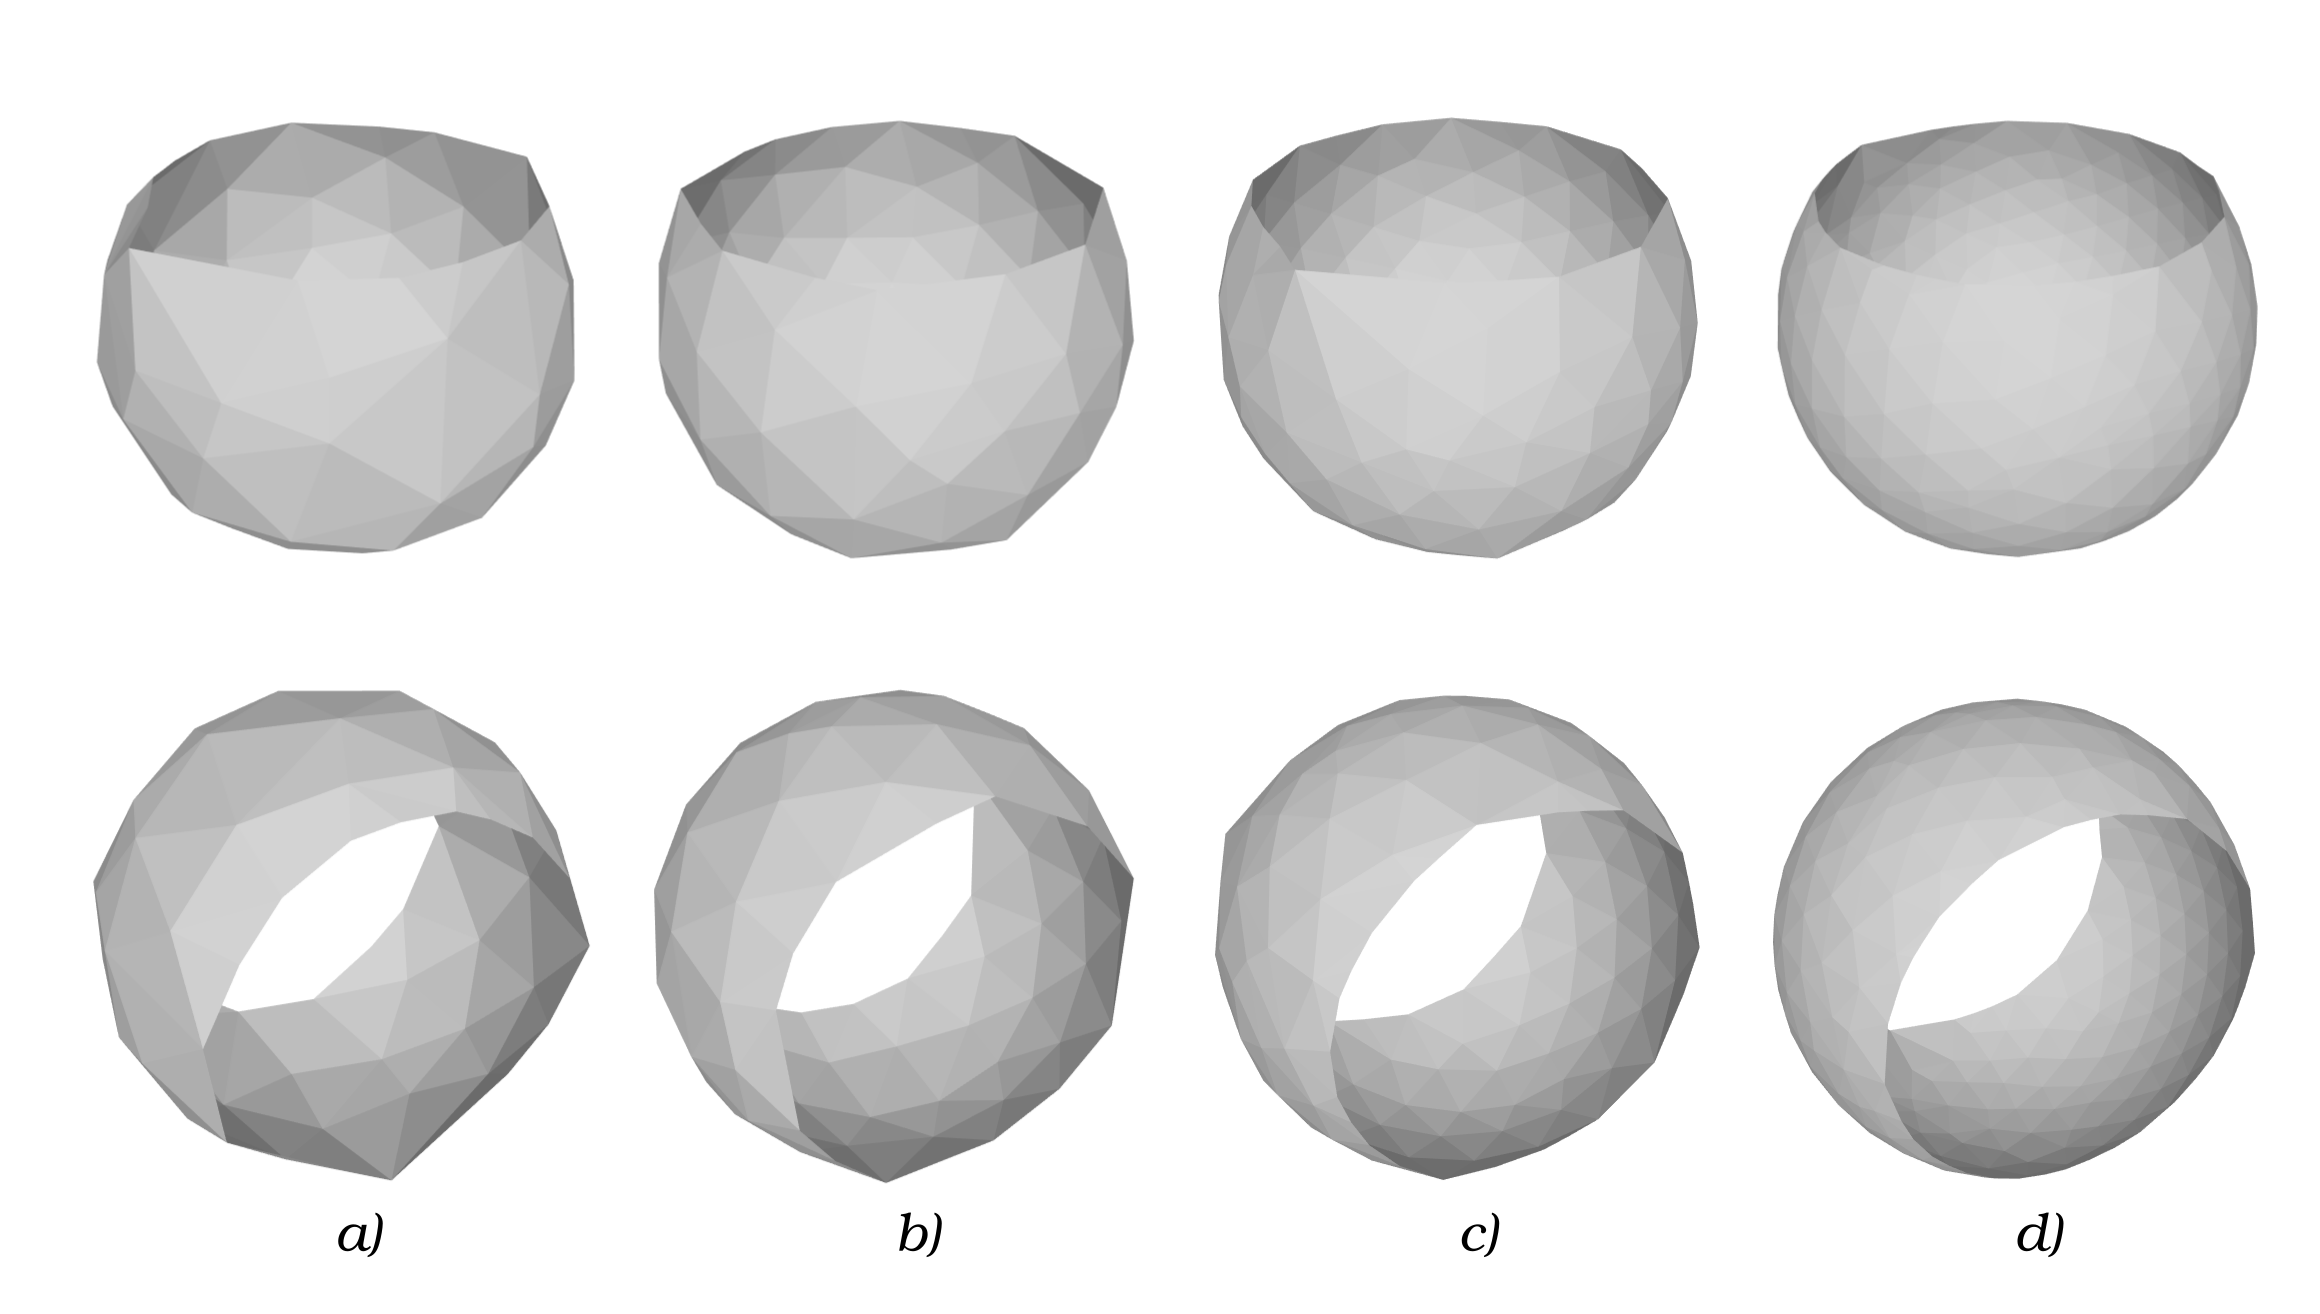
\includegraphics[width=0.8\textwidth]{images/cut_sphere}}
    \caption[Ohraničená triangulácia gule -- premietanie v smere ťažnice]
    {Premietanie v smere ťažnice.}
    %id obrazku, pomocou ktoreho sa budeme na obrazok odvolavat
    \label{obr:cut_sphere}
\end{figure}

Nie je však pravda, že pripínanie na obálku v smere ťažnice je vždy lepšie.
Pripínanie v smere ťažnice má nevýhodu vytváranie užších trojuholníkov pri 
okraji. Pripínanie na najbližší bod má zase nevýhodu, že smer premietania
nie je vždy v smere podobnom dotyčnici plochy.
Niektoré plochy však nemajú takúto nevýhodu.
Sú to plochy, ktoré majú v mieste orezania dotyčnicu približne v smere normály.
Pre takéto plochy býva prichytávanie v smere normály kvalitnejšie ako 
prichytávanie v smere ťažnice.

Toto správanie môžeme vidieť na obrázku \ref{obr:cylinder} a obrázku \ref{obr:cylinder_normal}, 
os valca je rovnobežná s jednou zo súradnicových osí.

Na obrázku \ref{obr:cylinder} vidíme orezaný valec, pričom používame
pripínanie na obálku v smere ťažnice. Na okraji môžeme vidieť užšie trojuholníky. 
Kdežto na obrázku \ref{obr:cylinder_normal} vidíme ten istý valec, 
avšak na orezávanie používame pripínanie k najbližšiemu bodu obálky.
Vidíme že tento valec nemá na okraji veľmi úzke trojuholníky avšak 
nemá ani deformovaný okraj ako sme to pozorovali pri orezanej sfére.

\begin{figure}
    \centerline{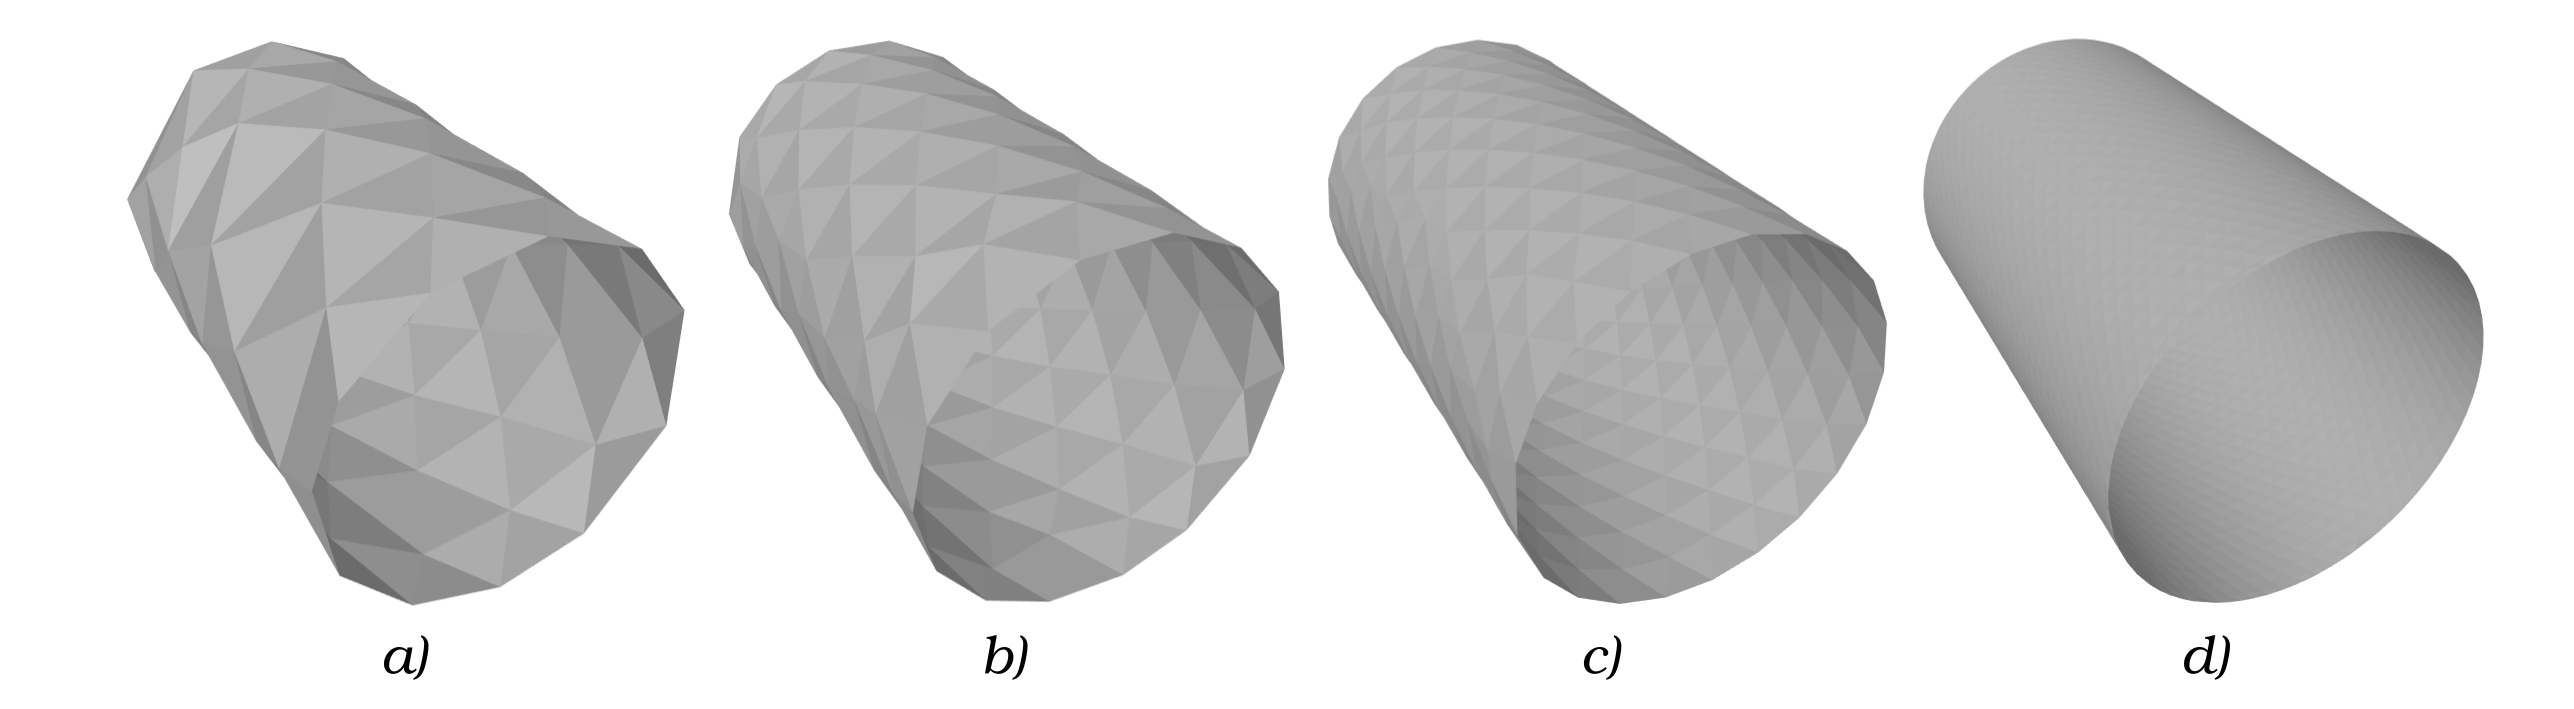
\includegraphics[width=1\textwidth]{images/cylinder_normal}}
    \caption[Ohraničená triangulácia tetrahedronu -- premietanie na najbližší bod]
    {Premietanie v smere ťažnice.}
    %id obrazku, pomocou ktoreho sa budeme na obrazok odvolavat
    \label{obr:cylinder_normal}
\end{figure}

\begin{figure}
    \centerline{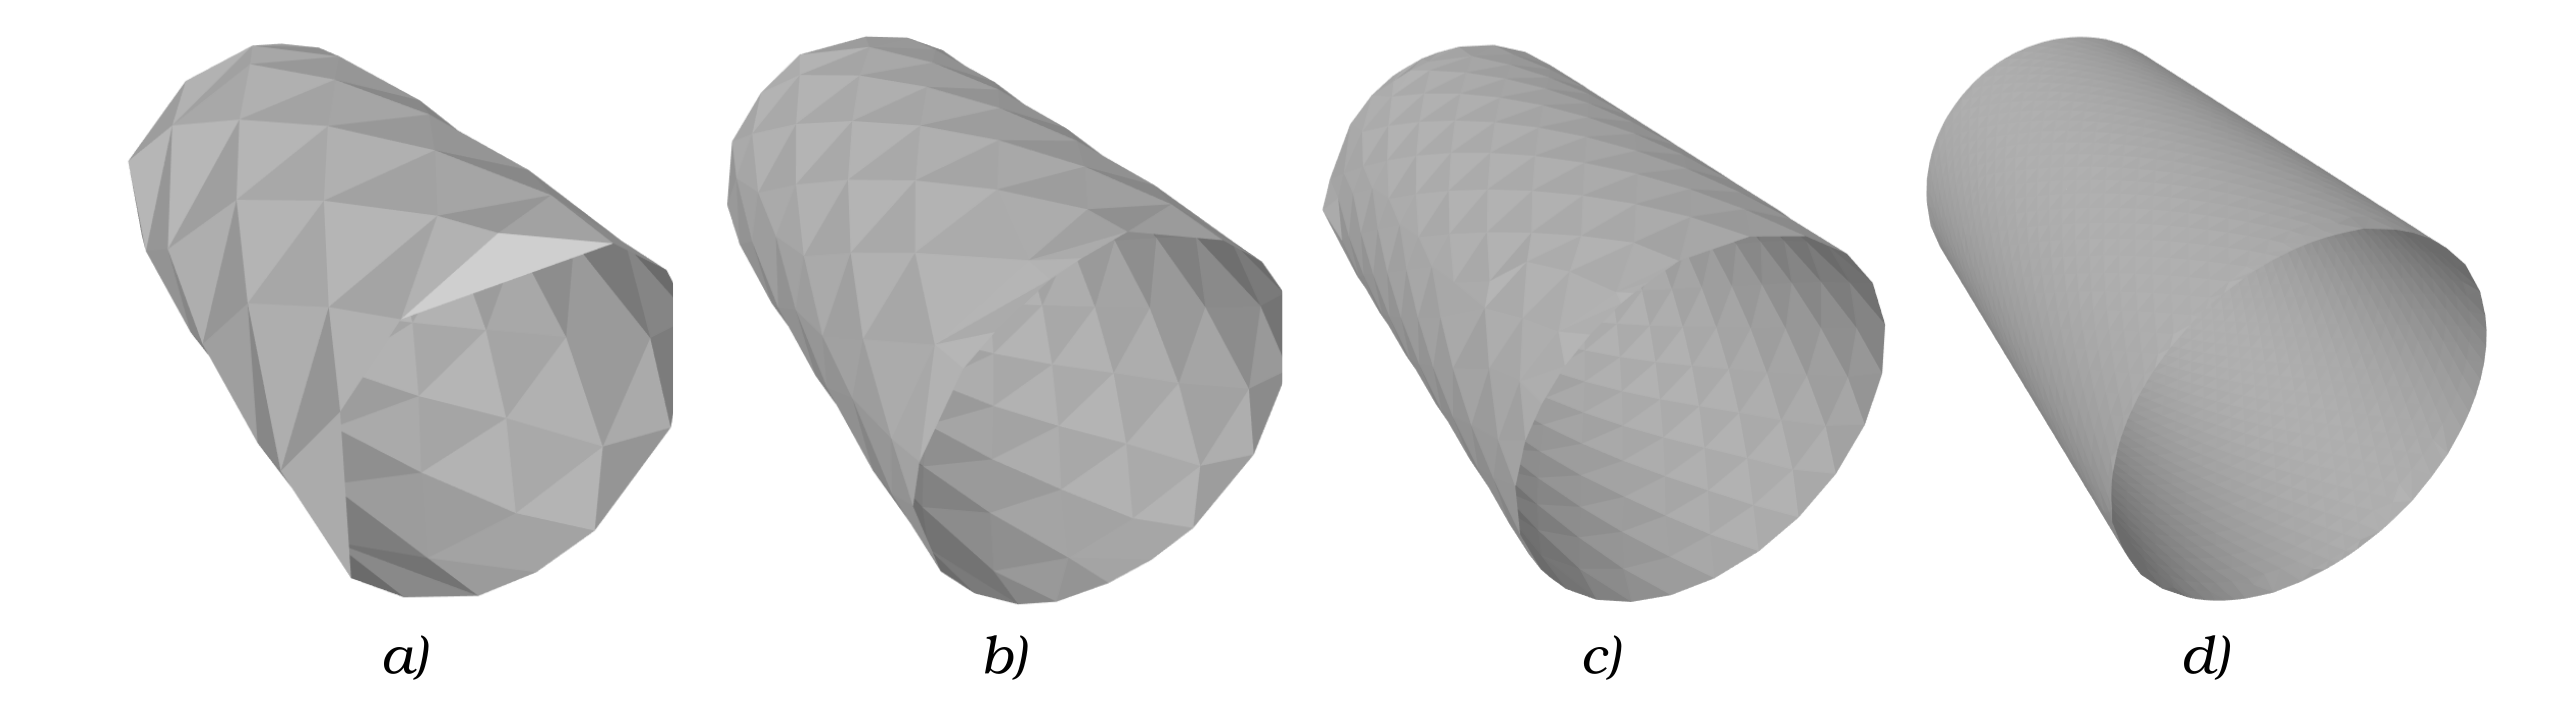
\includegraphics[width=1\textwidth]{images/cylinder}}
    \caption[Ohraničená triangulácia tetrahedronu -- premietanie v smere ťažnice]
    {Premietanie v smere ťažnice.}
    %id obrazku, pomocou ktoreho sa budeme na obrazok odvolavat
    \label{obr:cylinder}
\end{figure}


\subsection{Ohraničená triangulácia}

V tejto kapitole odprezentujeme výsledky dosiahnuté pri triangulácii plôch s použitím 
ohraničujúcej obálky. Ohraničujúcu obálku máme zadanú ako $3$--rozmerný interval 
$\langle x_{min}, x_{max}\rangle
\times \langle y_{min}, y_{max}\rangle \times \langle z_{min}, z_{max}\rangle \in \mathbb{R}^3.$ 
Modely v tejto časti orezávame pomocou prichytávania v smere ťažnice.

\begin{enumerate}

\newpage
\item{
    \textit{Eliptický paraboloid}

    \begin{equation}
    \label{eq:elliptic_paraboloid}
        x^2+y^2-2z = 0
    \end{equation}

    Plocha je ohraničená ohraničujúcou obálkou danou $3$--rozmerným intervalom 
    \newline
    \mbox{$\langle -10, 10 \rangle \times \langle -10, 10 \rangle \times \langle -10, 5 \rangle$}.

    Na obrázku \ref{obr:elliptic_paraboloid} vidíme výslednú trianguláciu eliptického paraboloidu
    daného implicitnou rovnicou \ref{eq:elliptic_paraboloid} so štyrmi rôznymi dĺžkami strany $a$.
    \begin{enumerate}[a)]
    \item{
        $a=1.000$, $n=216$, $p=121$
    }
    \item{
        $a=0.750$, $n=374$, $p=203$
    }
    \item{
        $a=0.500$, $n=778$, $p=409$
    }
    \item{
        $a=0.250$, $n=2980$, $p=1531$
    }
    \end{enumerate}

    \begin{figure}
        \centerline{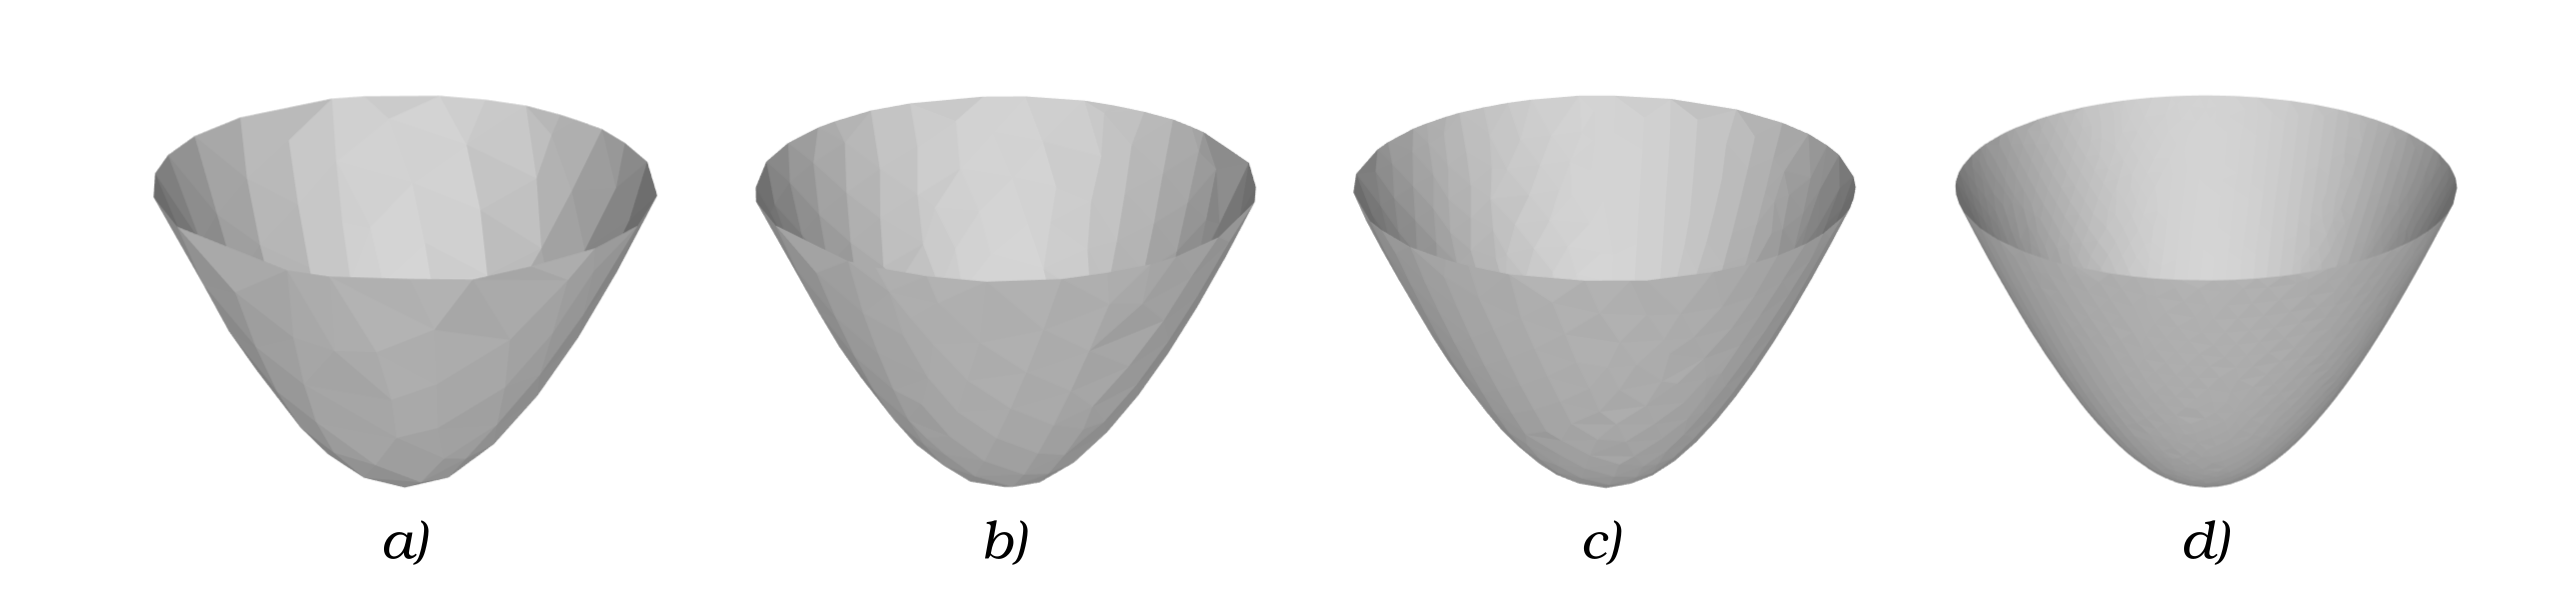
\includegraphics[width=1\textwidth]{images/elliptic_paraboloid}}
        \caption[Eliptický paraboloid]{Eliptický paraboloid}
        %id obrazku, pomocou ktoreho sa budeme na obrazok odvolavat
        \label{obr:elliptic_paraboloid}
    \end{figure}

    Výsledky merania kritérií kvality môžeme vidieť v tabuľke \ref{tab:elliptic_paraboloid}.

    \renewcommand*{\MinNumberA}{0.904}%
    \renewcommand*{\MaxNumberA}{0.969}%
    \pgfmathsetmacro{\MidNumberA}{(\MinNumberA+\MaxNumberA)/2}%
    \renewcommand*{\MinNumberB}{0.010}%
    \renewcommand*{\MaxNumberB}{0.034}%
    \pgfmathsetmacro{\MidNumberB}{(\MinNumberB+\MaxNumberB)/2}%
    \renewcommand*{\MinNumberC}{1.200}%
    \renewcommand*{\MaxNumberC}{1.373}%
    \pgfmathsetmacro{\MidNumberC}{(\MinNumberC+\MaxNumberC)/2}%
    \renewcommand*{\MinNumberD}{0.039}%
    \renewcommand*{\MaxNumberD}{0.094}%
    \pgfmathsetmacro{\MidNumberD}{(\MinNumberD+\MaxNumberD)/2}%
    \renewcommand*{\MinNumberE}{0.001}%
    \renewcommand*{\MaxNumberE}{0.041}%
    \pgfmathsetmacro{\MidNumberE}{(\MinNumberE+\MaxNumberE)/2}%
    \renewcommand*{\MinNumberF}{0.144}%
    \renewcommand*{\MaxNumberF}{0.422}%
    \pgfmathsetmacro{\MidNumberF}{(\MinNumberF+\MaxNumberF)/2}%
    \renewcommand*{\MinNumberG}{0.896}%
    \renewcommand*{\MaxNumberG}{0.966}%
    \pgfmathsetmacro{\MidNumberG}{(\MinNumberG+\MaxNumberG)/2}%
    \renewcommand*{\MinNumberH}{0.089}%
    \renewcommand*{\MaxNumberH}{0.147}%
    \pgfmathsetmacro{\MidNumberH}{(\MinNumberH+\MaxNumberH)/2}%


    \begin{table}[ht]
     \label{tab:elliptic_paraboloid}
     \caption[Výsledky merania triangulácie eliptického paraboloidu]{Výsledky merania}
        \begin{center}
            \begin{tabular}{|c|A B C D E F G H|}
                \hline
                \multicolumn{9}{|c|}{Eliptický paraboloid} \\
                \hline
                $\hspace{8mm} a \hspace{8mm}$ & $k_1$ & $k_2$ & $k_3$ & $k_4$ & $k_5$ & $k_6$ & $k_7$ & $k_8$ \EndTableHeader\\
                \hline
                1.000 & 0.904 & 0.034 & 1.373 & 0.094 & 0.013 & 0.422 & 0.896 & 0.147\\
                \hline
                0.750 & 0.912 & 0.027 & 1.296 & 0.086 & 0.041 & 0.354 & 0.904 & 0.125\\
                \hline
                0.500 & 0.953 & 0.019 & 1.269 & 0.069 & 0.011 & 0.261 & 0.951 & 0.116\\
                \hline
                0.250 & 0.969 & 0.010 & 1.200 & 0.039 & 0.001 & 0.144 & 0.966 & 0.089\\
                \hline
                \hline
            \end{tabular}
        \end{center}
    \end{table}

}
\newpage
\item{
    \textit{Hyperbolický paraboloid}

    \begin{equation}
    \label{eq:hyperbolic_paraboloid}
        x^2-y^2+2z = 0
    \end{equation}

    Plocha je ohraničená ohraničujúcou obálkou danou $3$--rozmerným intervalom 
    \newline
    \mbox{$\langle -3, 3 \rangle \times \langle -3, 3 \rangle \times \langle -20, 20 \rangle$}.

    Na obrázku \ref{obr:hyperbolic_paraboloid} vidíme výslednú trianguláciu hyperbolického paraboloidu
    daného implicitnou rovnicou \ref{eq:hyperbolic_paraboloid} so štyrmi rôznymi dĺžkami strany $a$.
    \begin{enumerate}[a)]
    \item{
        $a=1.000$, $n=205$, $p=121$
    }
    \item{
        $a=0.750$, $n=380$, $p=218$
    }
    \item{
        $a=0.500$, $n=845$, $p=464$
    }
    \item{
        $a=0.250$, $n=3359$, $p=1767$
    }
    \end{enumerate}

    \begin{figure}
        \centerline{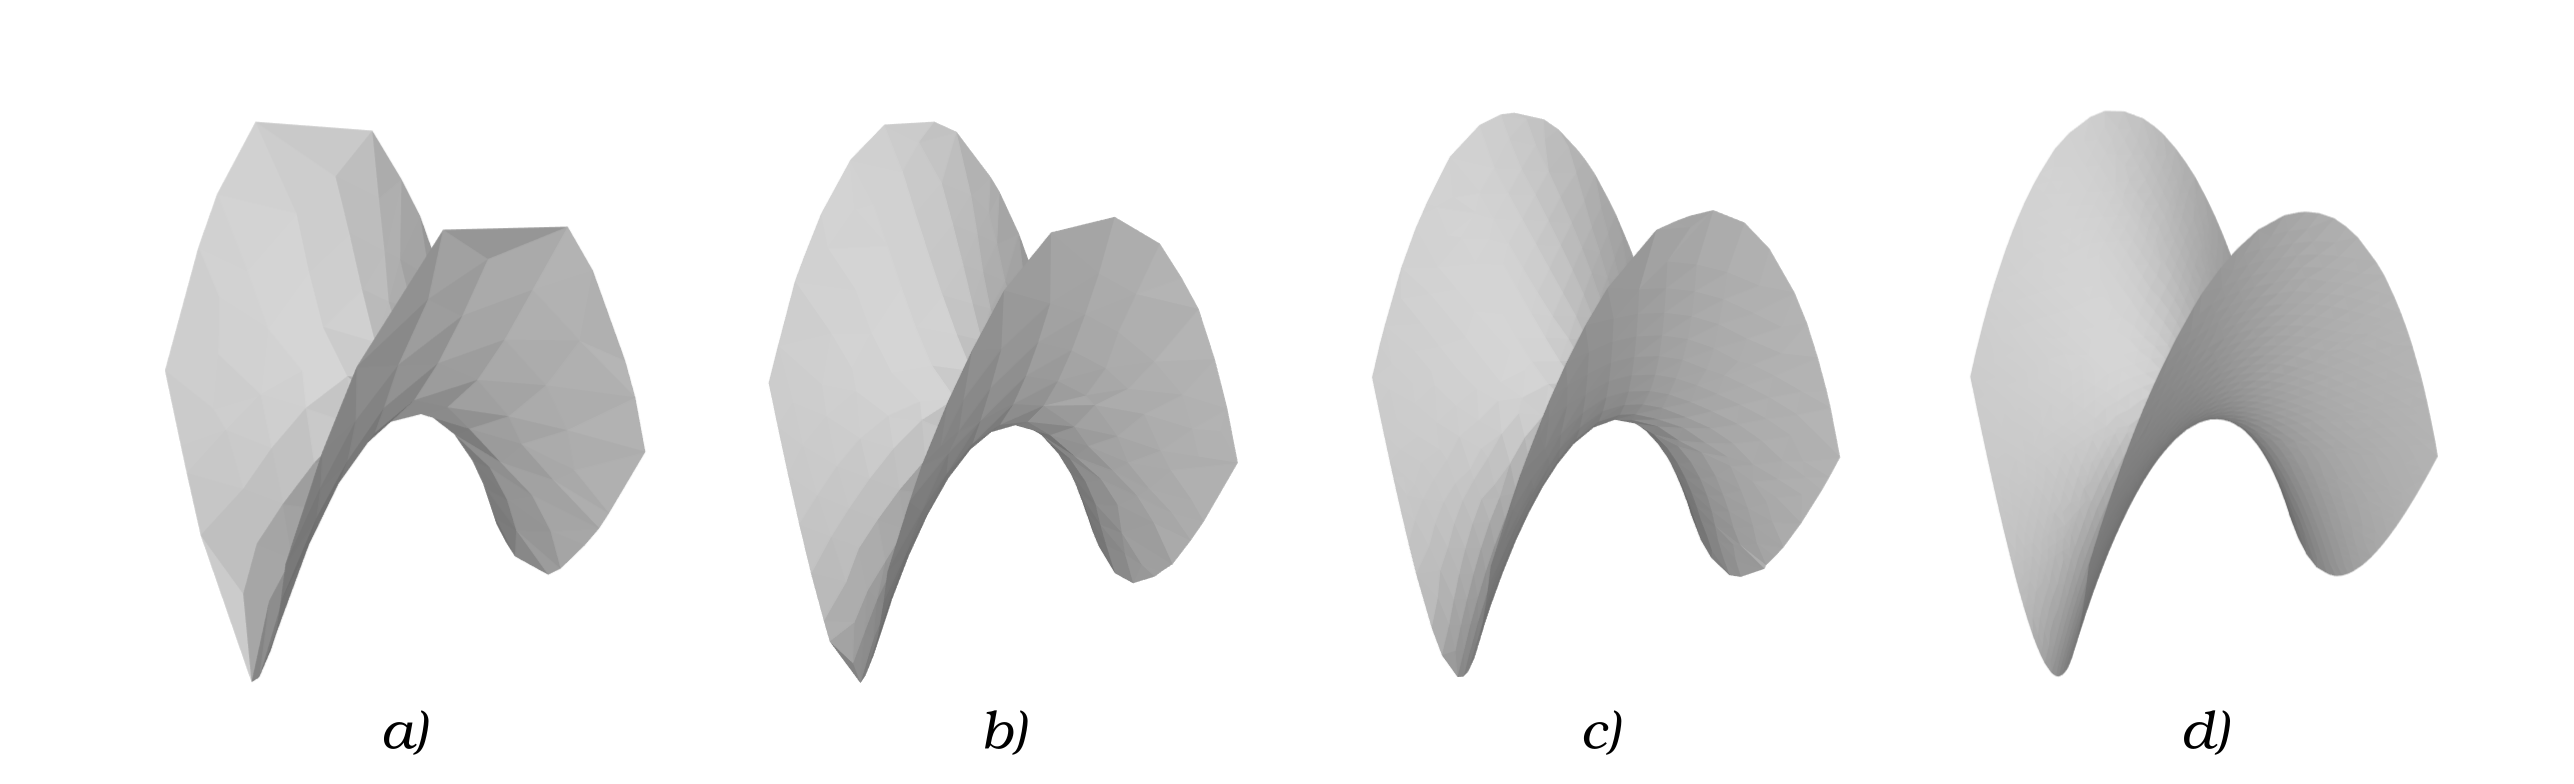
\includegraphics[width=1\textwidth]{images/hyperbolic_paraboloid}}
        \caption[Hyperbolický paraboloid]{Hyperbolický paraboloid}
        %id obrazku, pomocou ktoreho sa budeme na obrazok odvolavat
        \label{obr:hyperbolic_paraboloid}
    \end{figure}

    Výsledky merania kritérií kvality môžeme vidieť v tabuľke \ref{tab:hyperbolic_paraboloid}.

    \renewcommand*{\MinNumbera}{1.014}%
    \renewcommand*{\MaxNumbera}{1.046}%
    \pgfmathsetmacro{\MidNumbera}{(\MinNumbera+\MaxNumbera)/2}%
    \renewcommand*{\MinNumberB}{0.004}%
    \renewcommand*{\MaxNumberB}{0.017}%
    \pgfmathsetmacro{\MidNumberB}{(\MinNumberB+\MaxNumberB)/2}%
    \renewcommand*{\MinNumberC}{1.209}%
    \renewcommand*{\MaxNumberC}{1.363}%
    \pgfmathsetmacro{\MidNumberC}{(\MinNumberC+\MaxNumberC)/2}%
    \renewcommand*{\MinNumberD}{0.022}%
    \renewcommand*{\MaxNumberD}{0.144}%
    \pgfmathsetmacro{\MidNumberD}{(\MinNumberD+\MaxNumberD)/2}%
    \renewcommand*{\MinNumberE}{0.002}%
    \renewcommand*{\MaxNumberE}{0.032}%
    \pgfmathsetmacro{\MidNumberE}{(\MinNumberE+\MaxNumberE)/2}%
    \renewcommand*{\MinNumberF}{0.520}%
    \renewcommand*{\MaxNumberF}{1.259}%
    \pgfmathsetmacro{\MidNumberF}{(\MinNumberF+\MaxNumberF)/2}%
    \renewcommand*{\MinNumberg}{1.011}%
    \renewcommand*{\MaxNumberg}{1.056}%
    \pgfmathsetmacro{\MidNumberg}{(\MinNumberg+\MaxNumberg)/2}%
    \renewcommand*{\MinNumberH}{0.104}%
    \renewcommand*{\MaxNumberH}{0.200}%
    \pgfmathsetmacro{\MidNumberH}{(\MinNumberH+\MaxNumberH)/2}%


    \begin{table}[ht]
     \label{tab:hyperbolic_paraboloid}
     \caption[Výsledky merania triangulácie Hyperbolického paraboloidu]{Výsledky merania}
        \begin{center}
            \begin{tabular}{|c|a B C D E F g H|}
                \hline
                \multicolumn{9}{|c|}{Hyperbolický paraboloid} \\
                \hline
                $\hspace{8mm} a \hspace{8mm}$ & $k_1$ & $k_2$ & $k_3$ & $k_4$ & $k_5$ & $k_6$ & $k_7$ & $k_8$ \EndTableHeader\\
                \hline
                1.000 & 1.046 & 0.017 & 1.363 & 0.144 & 0.010 & 0.860 & 1.056 & 0.200\\
                \hline
                0.750 & 1.015 & 0.011 & 1.313 & 0.095 & 0.032 & 1.259 & 1.012 & 0.160\\
                \hline
                0.500 & 1.016 & 0.008 & 1.259 & 0.040 & 0.006 & 0.520 & 1.013 & 0.132\\
                \hline
                0.250 & 1.014 & 0.004 & 1.209 & 0.022 & 0.002 & 1.072 & 1.011 & 0.104\\
                \hline
                \hline
            \end{tabular}
        \end{center}
    \end{table}
}
\newpage
\item{
    \textit{Zovšeobecnený valec s parabolickým rezom}

    \begin{equation}
    \label{eq:parabolic_cylinder}
        x^2+2y = 0
    \end{equation}

    Plocha je ohraničená ohraničujúcou obálkou danou $3$--rozmerným intervalom 
    \newline
    \mbox{$\langle -5, 5 \rangle \times \langle -5, 5 \rangle \times \langle -5, 5 \rangle$}.

    Na obrázku \ref{obr:parabolic_cylinder} vidíme výslednú trianguláciu plochy
    danej implicitnou rovnicou \ref{eq:parabolic_cylinder} so štyrmi rôznymi dĺžkami strany $a$.
    \begin{enumerate}[a)]
    \item{
        $a=1.000$, $n=333$, $p=194$
    }
    \item{
        $a=0.750$, $n=564$, $p=313$
    }
    \item{
        $a=0.500$, $n=1215$, $p=658$
    }
    \item{
        $a=0.250$, $n=4656$, $p=2417$
    }
    \end{enumerate}

    \begin{figure}
        \centerline{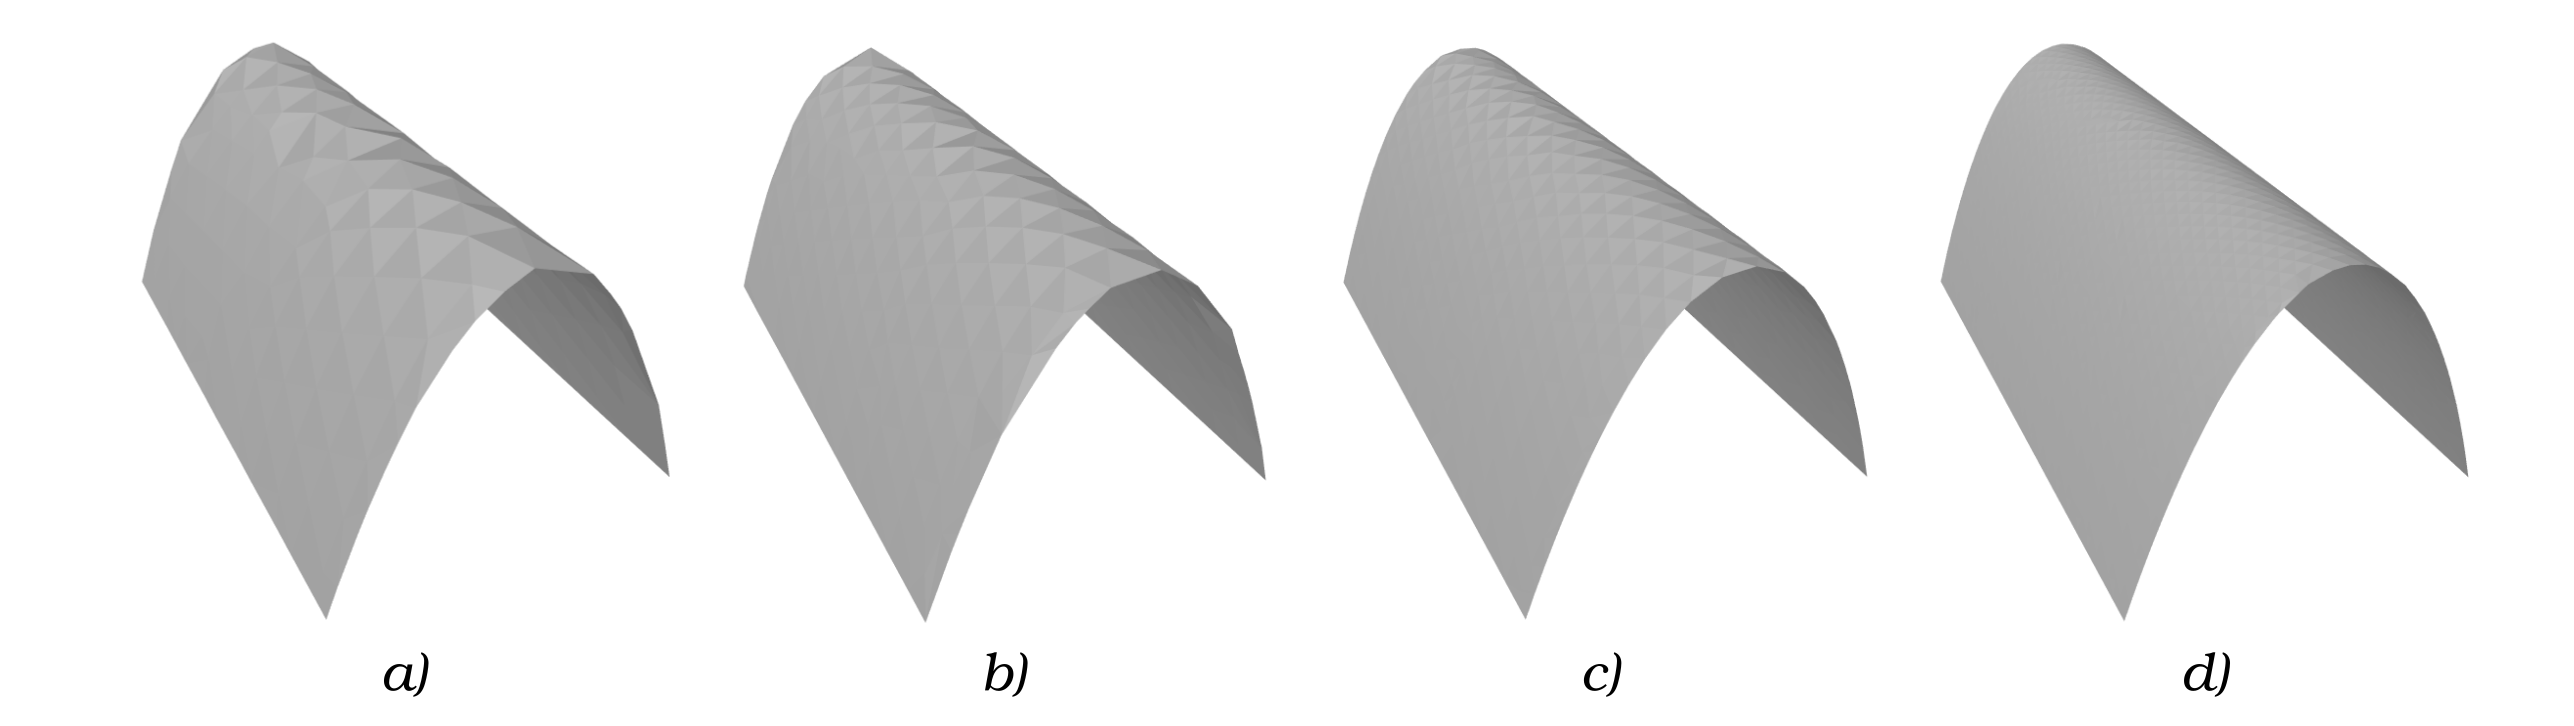
\includegraphics[width=1\textwidth]{images/parabolic_cylinder}}
        \caption[Triangulácia zovšeobecneného valca s parabolickým rezom]
        {Triangulácia zovšeobecneného valca s parabolickým rezom.}
        %id obrazku, pomocou ktoreho sa budeme na obrazok odvolavat
        \label{obr:parabolic_cylinder}
    \end{figure}

    Výsledky merania kritérií kvality môžeme vidieť v tabuľke \ref{tab:parabolic_cylinder}.

    \renewcommand*{\MinNumberA}{0.938}%
    \renewcommand*{\MaxNumberA}{1.005}%
    \pgfmathsetmacro{\MidNumberA}{(\MinNumberA+\MaxNumberA)/2}%
    \renewcommand*{\MinNumberB}{0.004}%
    \renewcommand*{\MaxNumberB}{0.015}%
    \pgfmathsetmacro{\MidNumberB}{(\MinNumberB+\MaxNumberB)/2}%
    \renewcommand*{\MinNumberC}{1.131}%
    \renewcommand*{\MaxNumberC}{1.302}%
    \pgfmathsetmacro{\MidNumberC}{(\MinNumberC+\MaxNumberC)/2}%
    \renewcommand*{\MinNumberD}{0.031}%
    \renewcommand*{\MaxNumberD}{0.108}%
    \pgfmathsetmacro{\MidNumberD}{(\MinNumberD+\MaxNumberD)/2}%
    \renewcommand*{\MinNumberE}{0.000}%
    \renewcommand*{\MaxNumberE}{0.141}%
    \pgfmathsetmacro{\MidNumberE}{(\MinNumberE+\MaxNumberE)/2}%
    \renewcommand*{\MinNumberF}{0.243}%
    \renewcommand*{\MaxNumberF}{0.576}%
    \pgfmathsetmacro{\MidNumberF}{(\MinNumberF+\MaxNumberF)/2}%
    \renewcommand*{\MinNumberG}{0.923}%
    \renewcommand*{\MaxNumberG}{1.001}%
    \pgfmathsetmacro{\MidNumberG}{(\MinNumberG+\MaxNumberG)/2}%
    \renewcommand*{\MinNumberH}{0.074}%
    \renewcommand*{\MaxNumberH}{0.133}%
    \pgfmathsetmacro{\MidNumberH}{(\MinNumberH+\MaxNumberH)/2}%

    \begin{table}[ht]
     \label{tab:parabolic_cylinder}
     \caption[Výsledky merania triangulácie zovšeobecneného valca]{Výsledky merania}
        \begin{center}
            \begin{tabular}{|c|A B C D E F G H|}
                \hline
                \multicolumn{9}{|c|}{Zovšeobecnený valec s parabolickým rezom} \\
                \hline
                $\hspace{8mm} a \hspace{8mm}$ & $k_1$ & $k_2$ & $k_3$ & $k_4$ & $k_5$ & $k_6$ & $k_7$ & $k_8$ \EndTableHeader\\
                \hline
                1.000 & 0.938 & 0.015 & 1.302 & 0.108 & 0.141 & 0.576 & 0.923 & 0.133\\
                \hline
                0.750 & 0.966 & 0.012 & 1.248 & 0.102 & 0.041 & 2.836 & 0.957 & 0.120\\
                \hline
                0.500 & 0.975 & 0.009 & 1.147 & 0.082 & 0.003 & 0.349 & 0.967 & 0.075\\
                \hline
                0.250 & 1.005 & 0.004 & 1.131 & 0.031 & 0.000 & 0.243 & 1.001 & 0.074\\
                \hline
                \hline
            \end{tabular}
        \end{center}
    \end{table}
}
\newpage
\item{
    \textit{Regulárna časť kužeľa}

    \begin{equation}
    \label{eq:quadric_cone}
        x^2+y^2-z^2 = 0
    \end{equation}

    Plocha je ohraničená ohraničujúcou obálkou danou $3$--rozmerným intervalom 
    \newline
    \mbox{$\langle -10, 10 \rangle \times \langle -10, 10 \rangle \times \langle 1, 5 \rangle$}.

    Na obrázku \ref{obr:quadric_cone} vidíme výslednú trianguláciu regulárnej časti kužeľa
    daného implicitnou rovnicou \ref{eq:quadric_cone} so štyrmi rôznymi dĺžkami strany $a$.
    \begin{enumerate}[a)]
    \item{
        $a=1.000$, $n=274$, $p=156$
    }
    \item{
        $a=0.750$, $n=462$, $p=254$
    }
    \item{
        $a=0.500$, $n=1012$, $p=541$
    }
    \item{
        $a=0.250$, $n=4041$, $p=2100$
    }
    \end{enumerate}

    \begin{figure}
        \centerline{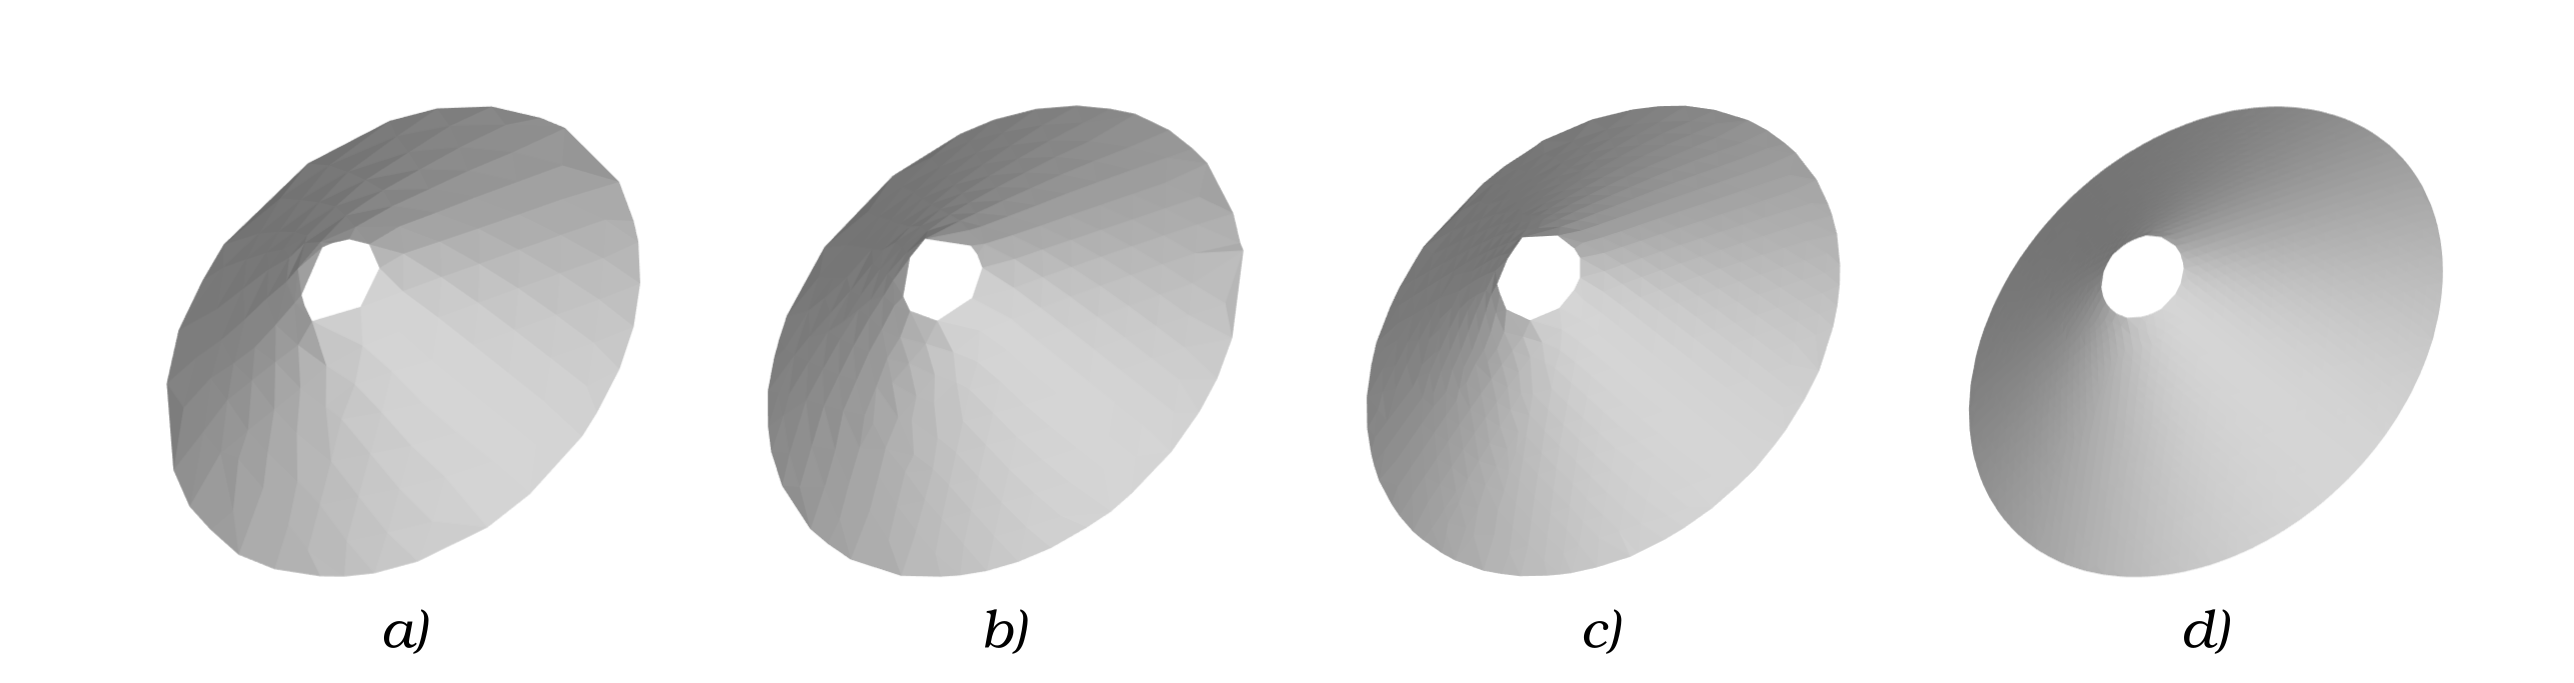
\includegraphics[width=1\textwidth]{images/quadric_cone}}
        \caption[Triangulácia regulárnej časti kužeľa]{Triangulácia regulárnej časti kužeľa.}
        %id obrazku, pomocou ktoreho sa budeme na obrazok odvolavat
        \label{obr:quadric_cone}
    \end{figure}

    Výsledky merania kritériu kvality môžeme vidieť v tabuľke \ref{tab:quadric_cone}.

    \renewcommand*{\MinNumberA}{0.960}%
    \renewcommand*{\MaxNumberA}{0.998}%
    \pgfmathsetmacro{\MidNumberA}{(\MinNumberA+\MaxNumberA)/2}%
    \renewcommand*{\MinNumberB}{0.005}%
    \renewcommand*{\MaxNumberB}{0.020}%
    \pgfmathsetmacro{\MidNumberB}{(\MinNumberB+\MaxNumberB)/2}%
    \renewcommand*{\MinNumberC}{1.114}%
    \renewcommand*{\MaxNumberC}{1.247}%
    \pgfmathsetmacro{\MidNumberC}{(\MinNumberC+\MaxNumberC)/2}%
    \renewcommand*{\MinNumberD}{0.042}%
    \renewcommand*{\MaxNumberD}{0.129}%
    \pgfmathsetmacro{\MidNumberD}{(\MinNumberD+\MaxNumberD)/2}%
    \renewcommand*{\MinNumberE}{0.000}%
    \renewcommand*{\MaxNumberE}{0.041}%
    \pgfmathsetmacro{\MidNumberE}{(\MinNumberE+\MaxNumberE)/2}%
    \renewcommand*{\MinNumberF}{0.196}%
    \renewcommand*{\MaxNumberF}{3.127}%
    \pgfmathsetmacro{\MidNumberF}{(\MinNumberF+\MaxNumberF)/2}%
    \renewcommand*{\MinNumberG}{0.954}%
    \renewcommand*{\MaxNumberG}{0.997}%
    \pgfmathsetmacro{\MidNumberG}{(\MinNumberG+\MaxNumberG)/2}%
    \renewcommand*{\MinNumberH}{0.055}%
    \renewcommand*{\MaxNumberH}{0.121}%
    \pgfmathsetmacro{\MidNumberH}{(\MinNumberH+\MaxNumberH)/2}%

    \begin{table}[ht]
     \label{tab:quadric_cone}
     \caption[Výsledky merania triangulácie regulárnej časti kužeľa]{Výsledky merania}
        \begin{center}
            \begin{tabular}{|c|A B C D E F G H|}
                \hline
                \multicolumn{9}{|c|}{Kužeľ} \\
                \hline
                $\hspace{8mm} a \hspace{8mm}$ & $k_1$ & $k_2$ & $k_3$ & $k_4$ & $k_5$ & $k_6$ & $k_7$ & $k_8$ \EndTableHeader\\
                \hline
                1.000 & 0.960 & 0.020 & 1.247 & 0.129 & 0.026 & 0.491 & 0.954 & 0.121\\
                \hline
                0.750 & 0.988 & 0.014 & 1.209 & 0.110 & 0.041 & 0.414 & 0.986 & 0.108\\
                \hline
                0.500 & 0.998 & 0.009 & 1.181 & 0.055 & 0.003 & 3.127 & 0.997 & 0.093\\
                \hline
                0.250 & 0.992 & 0.005 & 1.114 & 0.042 & 0.000 & 0.196 & 0.988 & 0.055\\
                \hline
                \hline
            \end{tabular}
        \end{center}
    \end{table}
}
\newpage
\item{
    \textit{Hyperboloid jedného plátu}

    \begin{equation}
    \label{eq:hyperboloid}
        x^2+y^2-z^2 -1 = 0
    \end{equation}

    Plocha je ohraničená ohraničujúcou obálkou danou $3$--rozmerným intervalom 
    \newline
    \mbox{$\langle -5, 5 \rangle \times \langle -5, 5 \rangle \times \langle -2, 2 \rangle$}.

    Na obrázku \ref{obr:hyperboloid} vidíme výslednú trianguláciu hyperboloidu
    daného implicitnou rovnicou \ref{eq:hyperboloid} so štyrmi rôznymi dĺžkami strany $a$.
    \begin{enumerate}[a)]
    \item{
        $a=1.000$, $n=144$, $p=87$
    }
    \item{
        $a=0.750$, $n=216$, $p=125$
    }
    \item{
        $a=0.500$, $n=454$, $p=255$
    }
    \item{
        $a=0.250$, $n=1727$, $p=917$
    }
    \end{enumerate}

    \begin{figure}
        \centerline{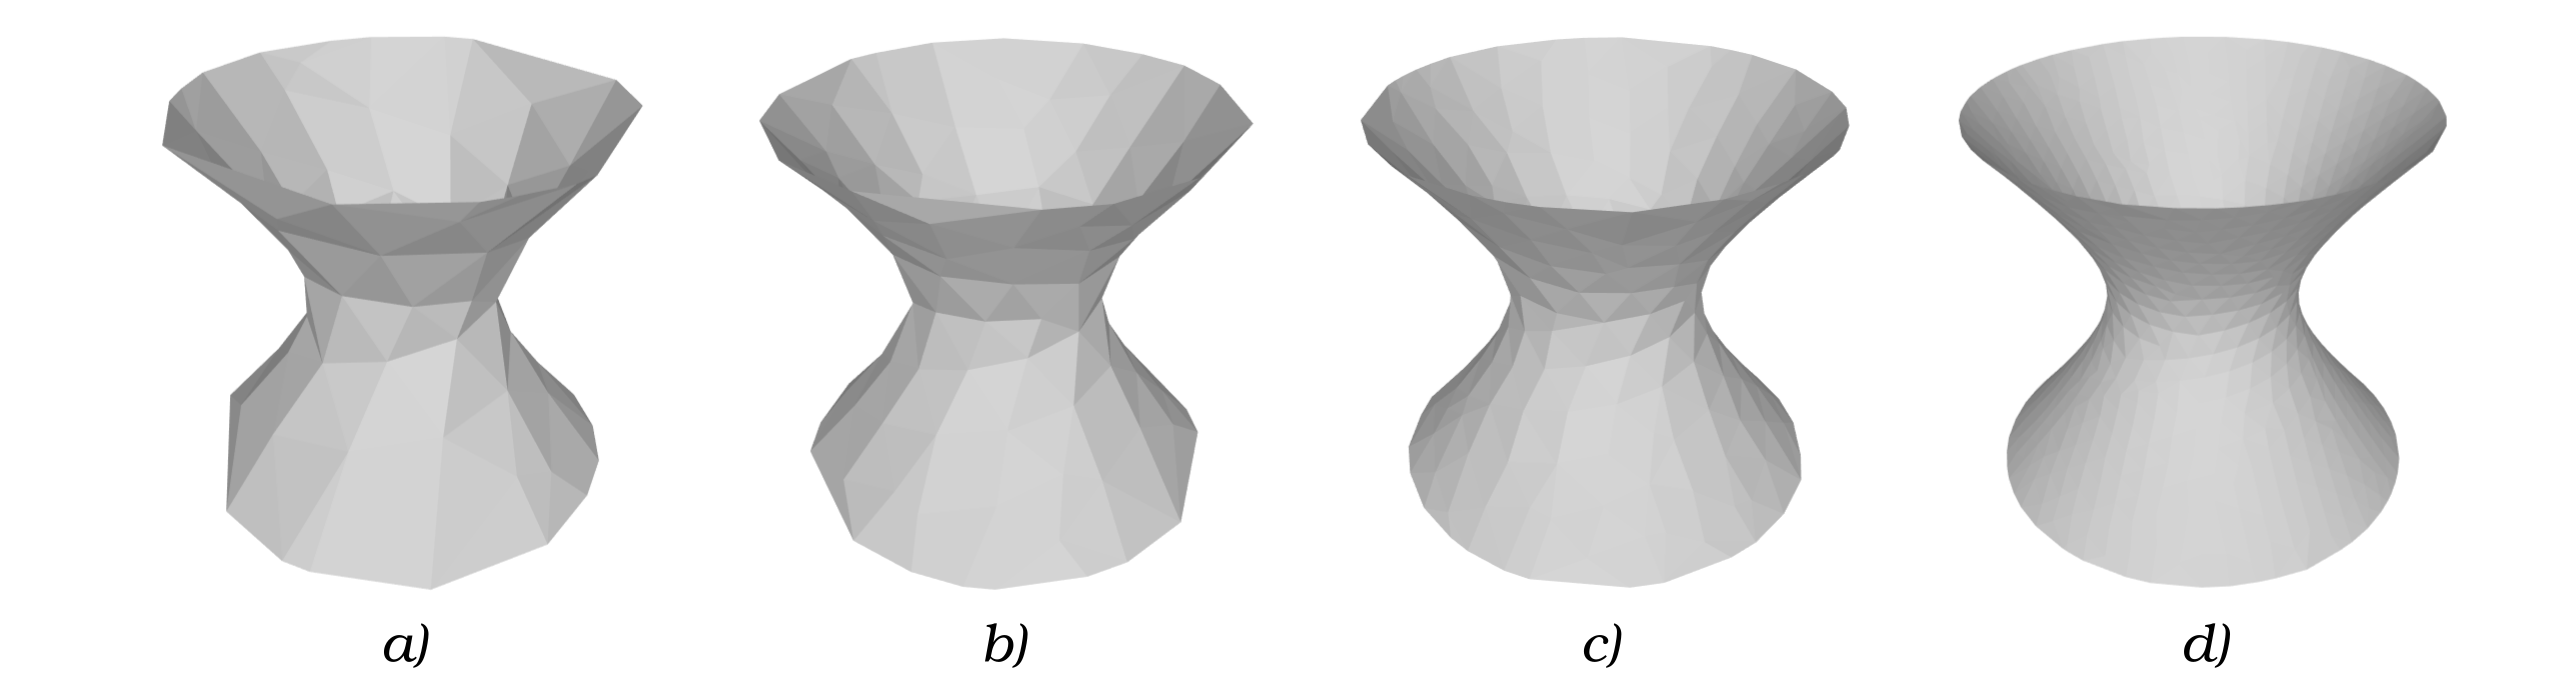
\includegraphics[width=1\textwidth]{images/hyperboloid}}
        \caption[Triangulácia hyperboloidu]{Triangulácia hyperboloidu.}
        %id obrazku, pomocou ktoreho sa budeme na obrazok odvolavat
        \label{obr:hyperboloid}
    \end{figure}

    Výsledky merania kritérií kvality môžeme vidieť v tabuľke \ref{tab:hyperboloid}.
    
    \renewcommand*{\MinNumberA}{0.877}%
    \renewcommand*{\MaxNumberA}{1.000}%
    \pgfmathsetmacro{\MidNumberA}{(\MinNumberA+\MaxNumberA)/2}%
    \renewcommand*{\MinNumberB}{0.007}%
    \renewcommand*{\MaxNumberB}{0.025}%
    \pgfmathsetmacro{\MidNumberB}{(\MinNumberB+\MaxNumberB)/2}%
    \renewcommand*{\MinNumberC}{1.225}%
    \renewcommand*{\MaxNumberC}{1.462}%
    \pgfmathsetmacro{\MidNumberC}{(\MinNumberC+\MaxNumberC)/2}%
    \renewcommand*{\MinNumberD}{0.043}%
    \renewcommand*{\MaxNumberD}{0.122}%
    \pgfmathsetmacro{\MidNumberD}{(\MinNumberD+\MaxNumberD)/2}%
    \renewcommand*{\MinNumberE}{0.003}%
    \renewcommand*{\MaxNumberE}{0.246}%
    \pgfmathsetmacro{\MidNumberE}{(\MinNumberE+\MaxNumberE)/2}%
    \renewcommand*{\MinNumberF}{0.319}%
    \renewcommand*{\MaxNumberF}{0.810}%
    \pgfmathsetmacro{\MidNumberF}{(\MinNumberF+\MaxNumberF)/2}%
    \renewcommand*{\MinNumberG}{0.869}%
    \renewcommand*{\MaxNumberG}{0.996}%
    \pgfmathsetmacro{\MidNumberG}{(\MinNumberG+\MaxNumberG)/2}%
    \renewcommand*{\MinNumberH}{0.108}%
    \renewcommand*{\MaxNumberH}{0.190}%
    \pgfmathsetmacro{\MidNumberH}{(\MinNumberH+\MaxNumberH)/2}%

    \begin{table}[ht]
     \label{tab:hyperboloid}
     \caption[Výsledky merania triangulácie hyperboloidu]{Výsledky merania}
        \begin{center}
            \begin{tabular}{|c|A B C D E F G H|}
                \hline
                \multicolumn{9}{|c|}{Hyperboloid} \\
                \hline
                $\hspace{8mm} a \hspace{8mm}$ & $k_1$ & $k_2$ & $k_3$ & $k_4$ & $k_5$ & $k_6$ & $k_7$ & $k_8$ \EndTableHeader\\
                \hline
                1.000 & 0.877 & 0.025 & 1.462 & 0.122 & 0.005 & 0.810 & 0.869 & 0.190\\
                \hline
                0.750 & 0.958 & 0.020 & 1.374 & 0.090 & 0.246 & 0.712 & 0.957 & 0.171\\
                \hline
                0.500 & 0.984 & 0.014 & 1.353 & 0.066 & 0.009 & 0.532 & 0.977 & 0.161\\
                \hline
                0.250 & 1.000 & 0.007 & 1.225 & 0.043 & 0.003 & 0.319 & 0.996 & 0.108\\
                \hline
                \hline
            \end{tabular}
        \end{center}
    \end{table}
}
\end{enumerate}

\section{Adaptívna triangulácia}
\subsection{Prerozdeľovanie trojuholníkov}

V našej práci sme implementovali jednu iteráciu adaptívneho prerozdelenia trojuholníkov
na miestach kde je ťažisko trojuholníka od plochy vzdialenejšie ako zvolená prahová hodnota $d$.

Na obrázku \ref{obr:adaptive_ellipsoid} vidíme trianguláciu elipsoidu so zvolenou dĺžkou hrany $a=0.7$
a následne výsledok adaptívneho prerozdelenia pre rôzne prahové hodnoty $d$.

\begin{figure}
    \centerline{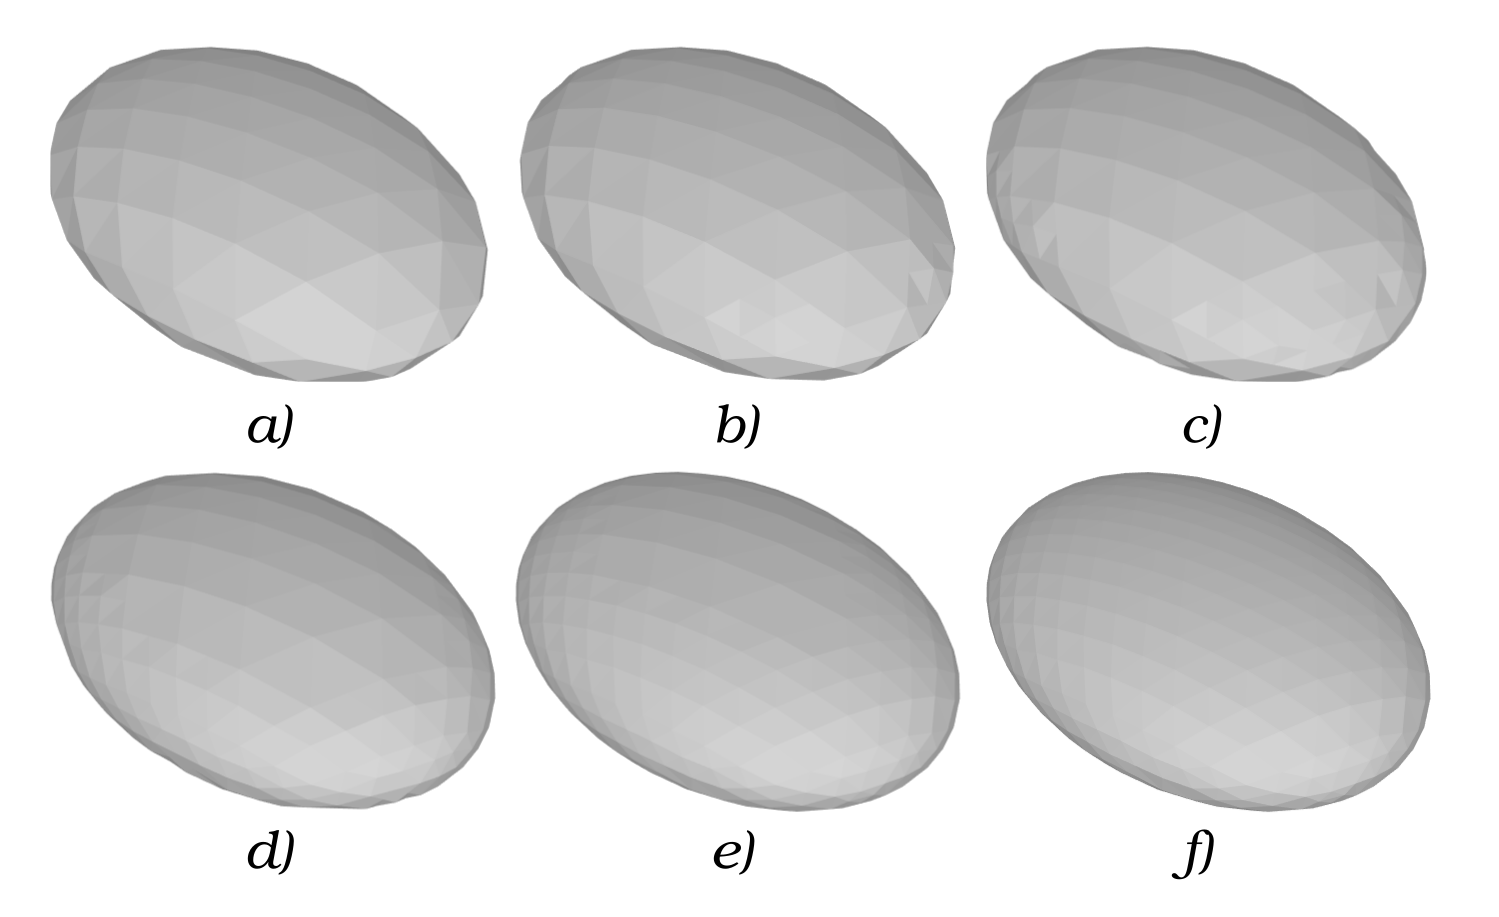
\includegraphics[width=0.6\textwidth]{images/adaptive_ellipsoid}}
    \caption[Adaptívne prerozdelenie elipsoidu.]
    {$a)$ bez adaptívneho prerozdelenia, $b)$ $d=0.05$, $c)$ $d=0.04$, $d)$ $d=0.03$, $e)$ $d=0.02$, $f)$ $d=0.01$}
    %id obrazku, pomocou ktoreho sa budeme na obrazok odvolavat
    \label{obr:adaptive_ellipsoid}
\end{figure}


Toto adaptívne prerozdelenie sme vyskúšali aj na nekonečnej ploche.
Na obrázku \ref{obr:adaptive_parabolic_cylinder} vidíme trianguláciu parabolického 
cylindra so zvolenou dĺžkou hrany $a=2$ a rôznymi prahovými hodnotami $d$.

\begin{figure}
    \centerline{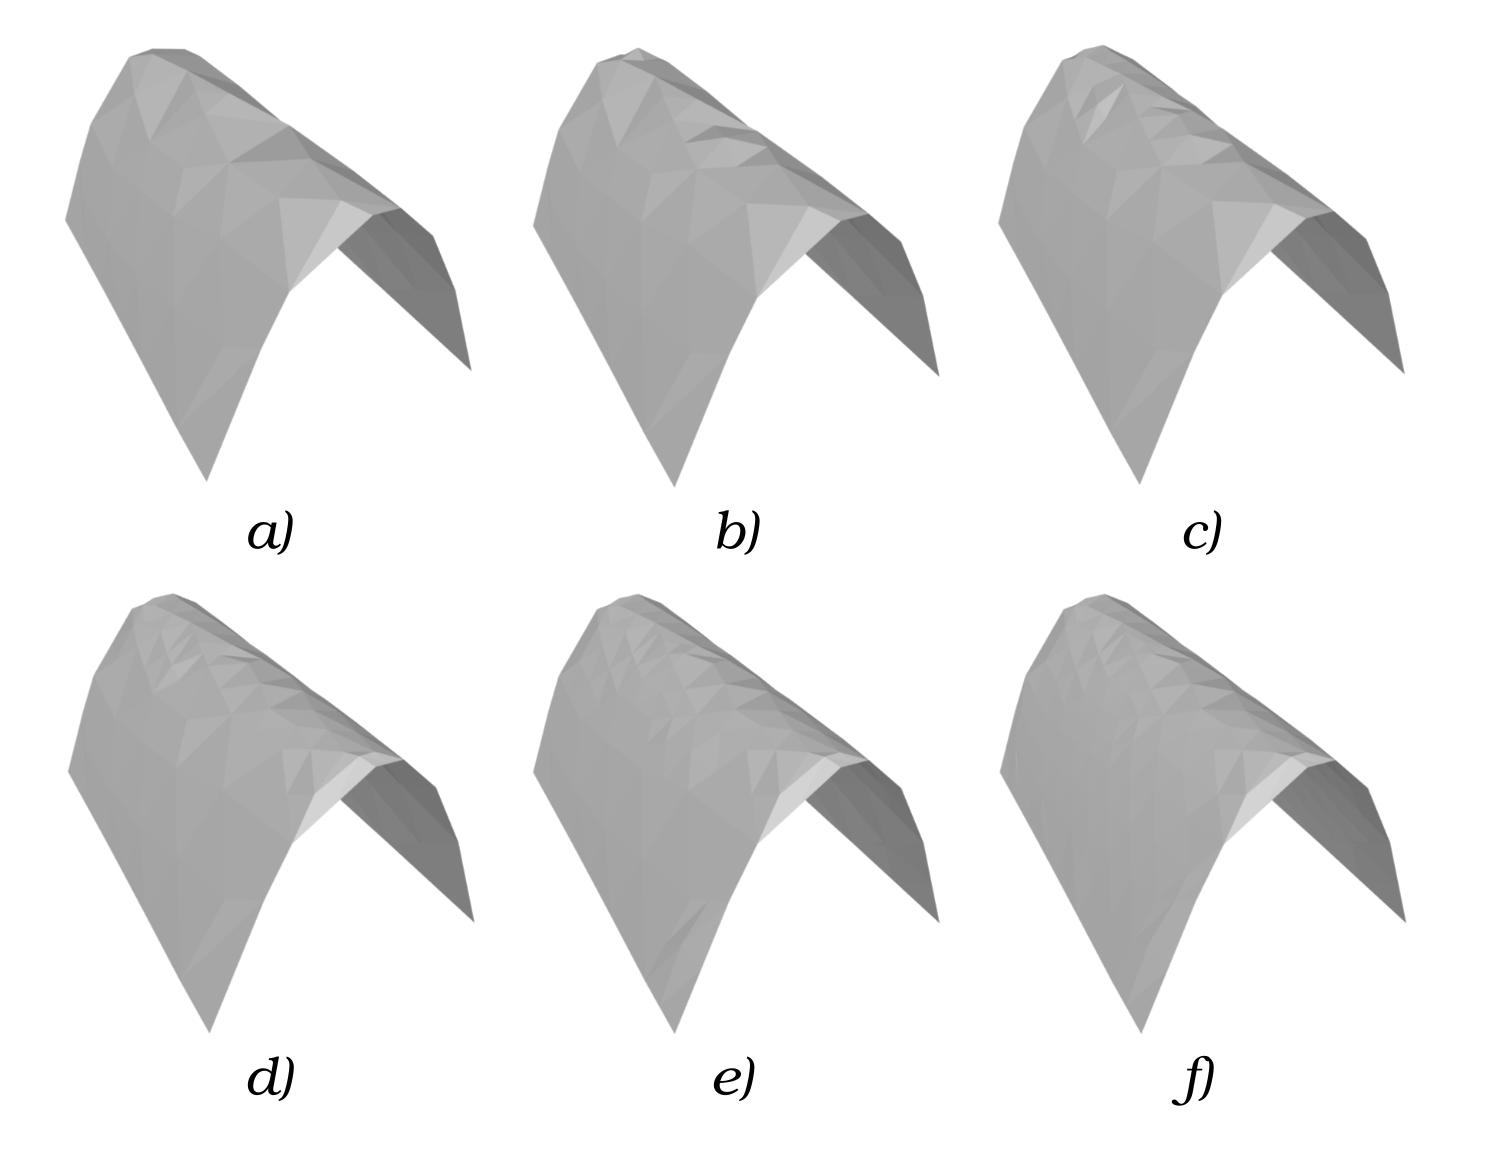
\includegraphics[width=0.6\textwidth]{images/adaptive_parabolic_cylinder}}
    \caption[Adaptívne prerozdelenie parabolického cylindra.]
    {$a)$ bez adaptívneho prerozdelenia, $b)$ $d=0.15$, $c)$ $d=0.1$, $d)$ $d=0.05$, $e)$ $d=0.03$, $f)$ $d=0.01$}
    %id obrazku, pomocou ktoreho sa budeme na obrazok odvolavat
    \label{obr:adaptive_parabolic_cylinder}
\end{figure}

\subsection{Prispôsobenie výšky nového trojuholníka}
Druhú metódu pre adaptívnu trianguláciu a to prispôsobenie výšky $k$ pri tvorbe nového trojuholníka 
vizualizujeme na niekoľkých modeloch.

Na modeloch pozorujeme, že pre vhodne zvolenú prahovú hodnotu $d$ nastáva prerozdeľovanie 
trojuholníkov v oblastiach s vyšším zakrivením, pričom trojuholníky v oblastiach s nižším zakrivením 
zostávajú zachované.

Na obrázku \ref{obr:adaptive_height_ellipsoid} vidíme trianguláciu elipsoidu so zvolenou
dĺžkou hrany $a=0.9$.
\begin{enumerate}[a)]
\item{
    Základný neadaptívny algoritmus, výška trojuholníka volená ako výška rovnostranného trojuholníka
    s dĺžkou hrany $a$, teda $h=\frac{\sqrt{3}}{2} a$.
}
\item{
    Výška nového trojuholníka volená na základe aktuálnej hrany. Označme jej dĺžku e, potom  
    $h=\frac{\sqrt{3}}{2} e$.
}
\item{
    Výška nového trojuholníka volená na základe priemernej dĺžky aktuálnej hrany a jej susedných hrán. 
    Označme dĺžky susedných strán $e_{prev}$ a $e_{next}$, potom  
    $h=\frac{\sqrt{3}}{2} \cdot \frac{e+e_{prev}+e_{next}}{3}$.
}
\item{
    Výška nového trojuholníka volená na základe priemernej dĺžky aktuálnej hrany a jej susedných hrán
    pričom zohľadňujeme vplyv zvolenej dĺžky hrany $a$. Teda
    $h=0.75(\frac{\sqrt{3}}{2} \cdot \frac{e+e_{prev}+e_{next}}{3}) + 0.25 a$.
}
\end{enumerate}


\begin{figure}
    \centerline{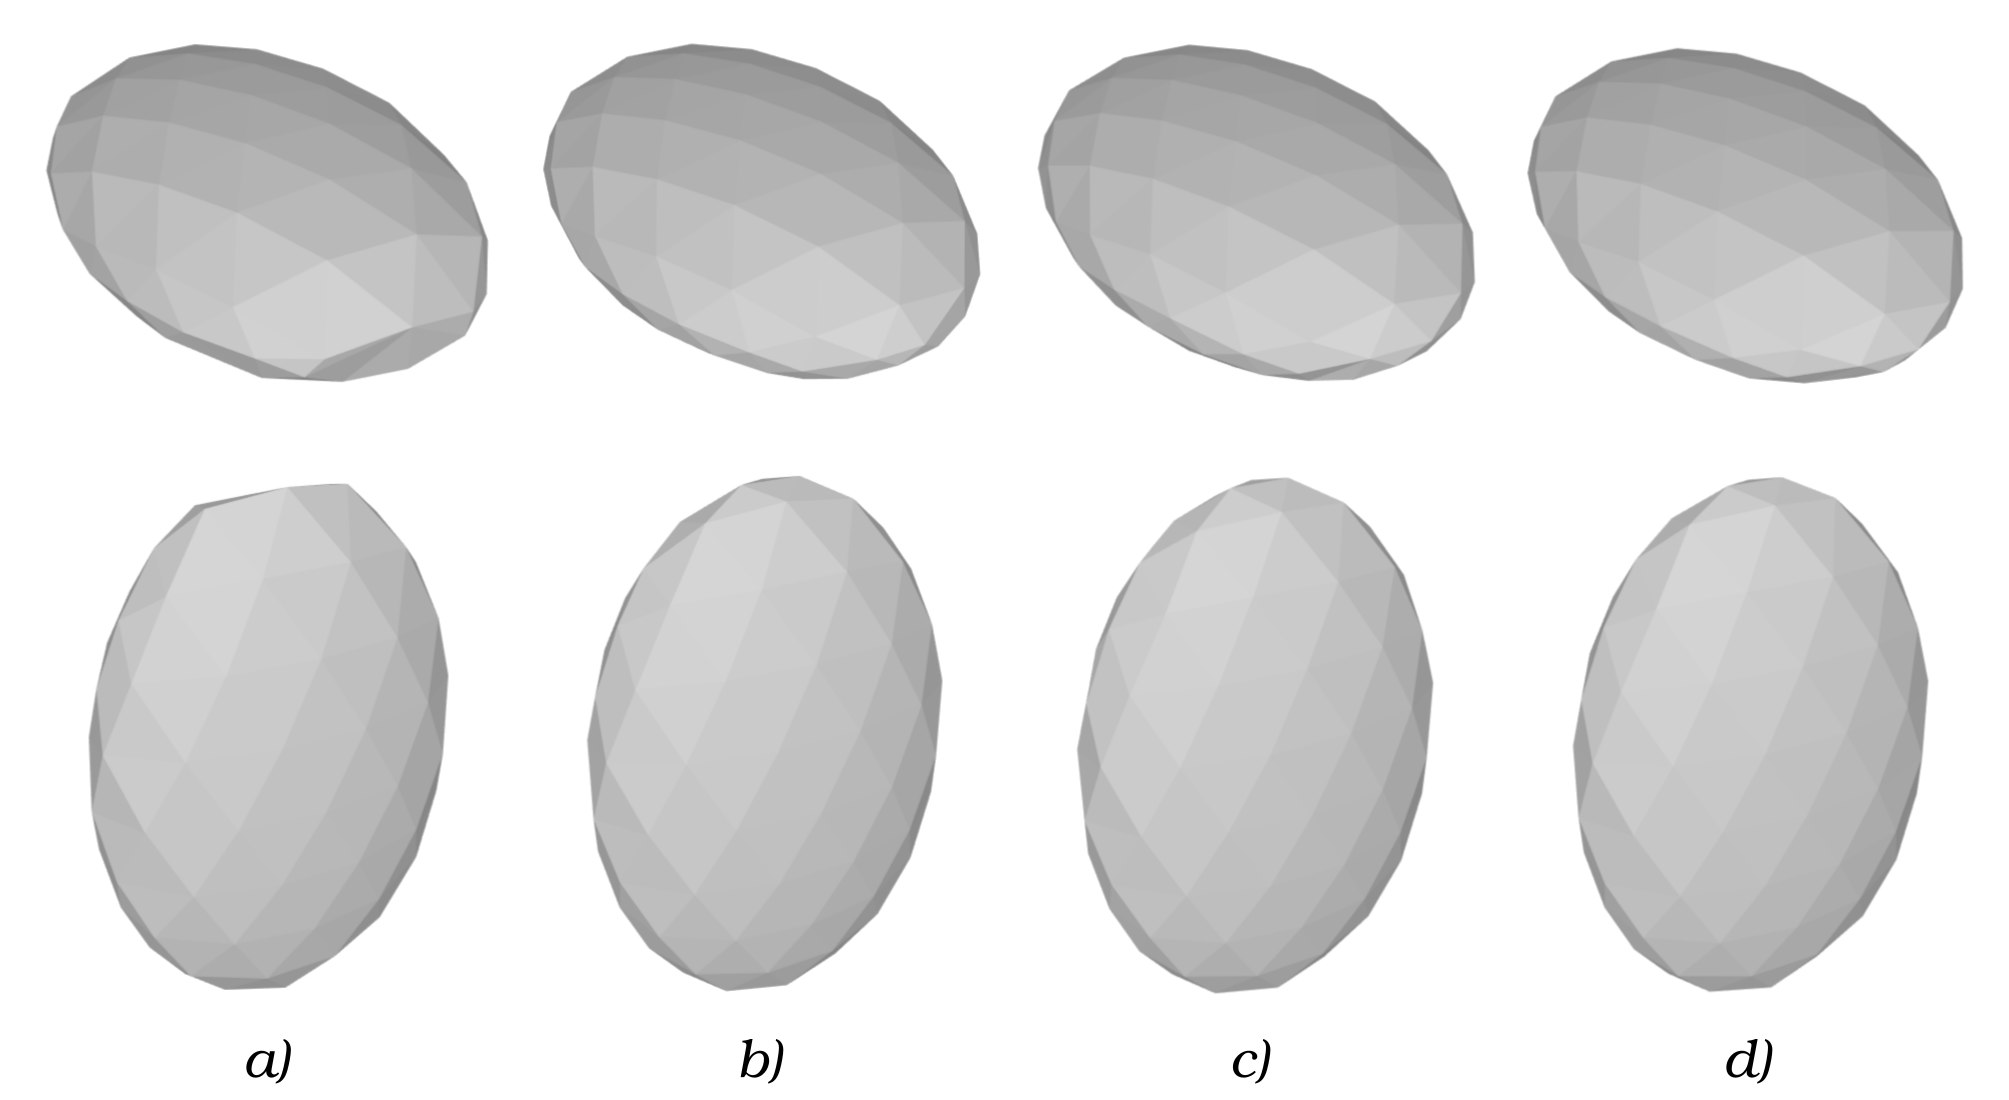
\includegraphics[width=0.8\textwidth]{images/adaptive_height_ellipsoid}}
    \caption[Adaptívna triangulácia elipsoidu]
    {Adaptívna triangulácia elipsoidu.}
    %id obrazku, pomocou ktoreho sa budeme na obrazok odvolavat
    \label{obr:adaptive_height_ellipsoid}
\end{figure}

Na obrázku \ref{obr:adaptive_height_tetrahedron} vidíme trianguláciu tetrahedronu so zvolenou
dĺžkou hrany $a=0.5$. Výšku nového trojuholníka volíme rovnako ako pri modeli elipsoidu.

\begin{figure}
    \centerline{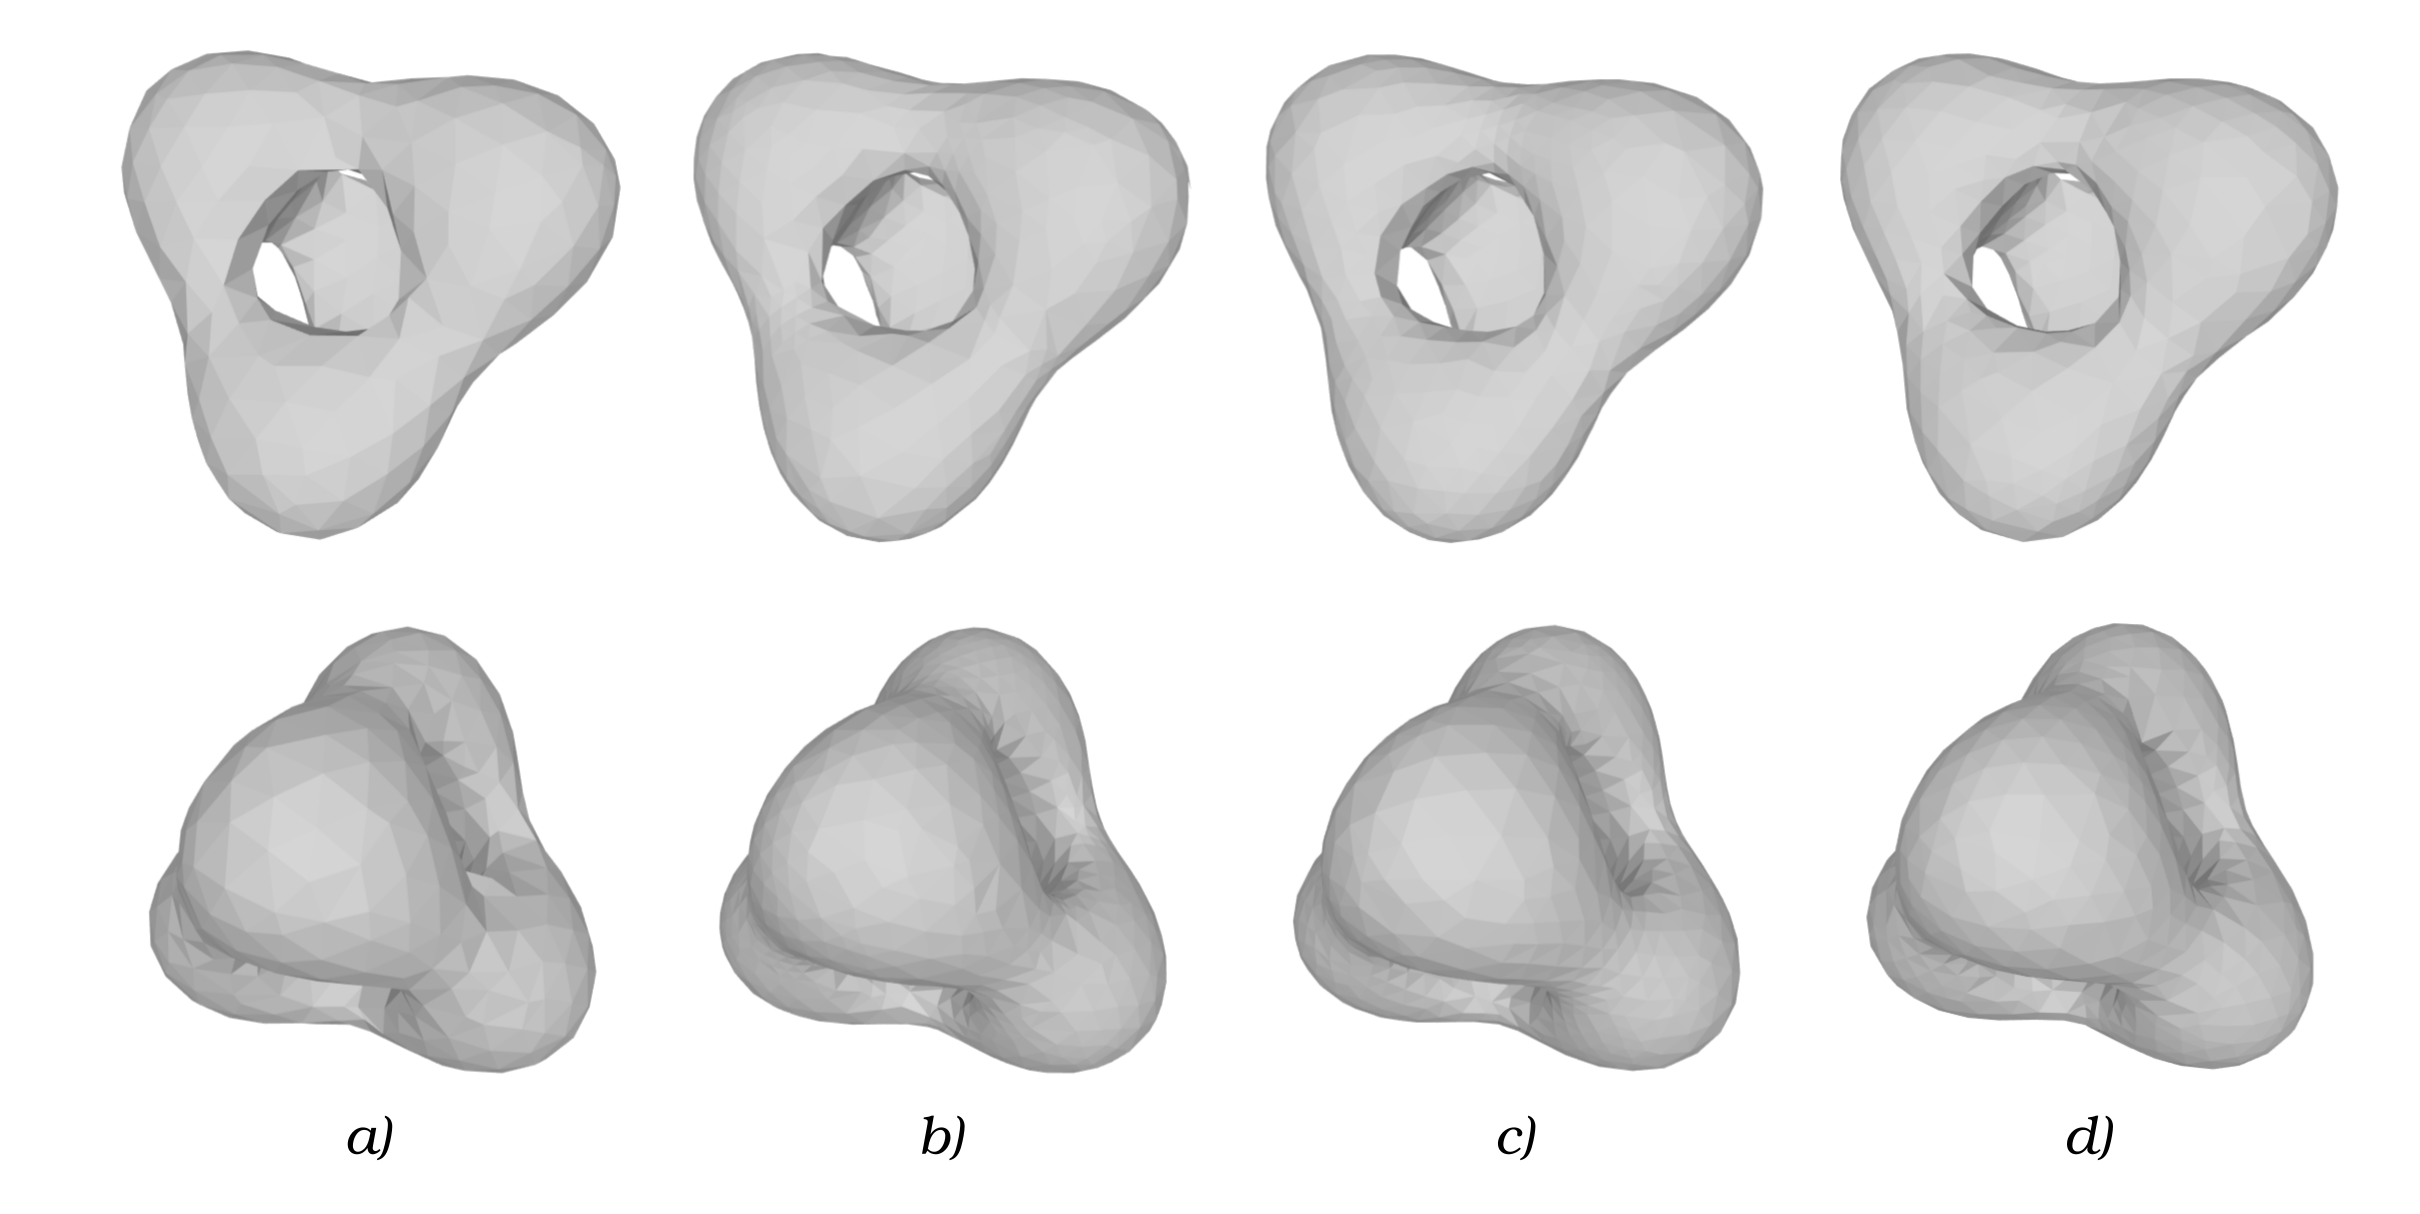
\includegraphics[width=0.9\textwidth]{images/adaptive_height_tetrahedron}}
    \caption[Adaptívna triangulácia tetrahedronu]
    {Adaptívna triangulácia tetrahedronu.}
    %id obrazku, pomocou ktoreho sa budeme na obrazok odvolavat
    \label{obr:adaptive_height_tetrahedron}
\end{figure}


\renewcommand{\arraystretch}{1}
\setlength{\fboxsep}{2mm} % box size
\setlength{\tabcolsep}{4pt}

    Nevýhoda, ktorú sme pozorovali pri výške založenej na aktuálnej hrane je občasné prekrývanie
    trojuholníkov, keďže \textit{Delaunayova podmienka} ani podmienka na zistenie blízkosti
    ťažiska nefungujú ideálne ak sa v triangulácii stretnú malý a veľký trojuholník.
    Ďalšou nevýhodou je veľké množstvo vznikajúcich trojuholníkov, keďže menšia hrana podmieňuje
    vznik menšieho trojuholníka a tento vplyv sa tak šíri ďalej.

    Pri prispôsobení výšky nového trojuholníka priemeru dĺžky aktuálnej hrany a dĺžok susedných 
    hrán pozorujeme už spomínanú nevýhodu. Trojuholníky zostávajú malé aj napriek tomu, že 
    sa už nenachádzajú v časti plochy s vyšším zakrivením a vytvára zbytočne veľké množstvo trojuholníkov.

    Tretí prístup eliminuje nevýhody oboch predchádzajúcich prístupov. Priemerovaním dĺžok hrán sa väčšinou 
    vyhneme stretnutiu veľmi malého a veľmi veľkého trojuholníka. Vplyvom zadanej dĺžky hrany pre 
    regióny s menším zakrivením trojuholníky opäť zväčšujeme a nevytvárame tak veľké množstvo zbytočných 
    trojuholníkov.

    Počty trojuholníkov jednotlivých triangulácii môžeme pozorovať v tabuľke \ref{tab:adaptive_height}.
    Vidíme, že všetky adaptívne prístupy generujú väčší počet trojuholníkov ako neadaptívna triangulácia,
    avšak tretí prístup má od prvého a druhého prístupu výrazne menší počet trojuholníkov. Najväčší
    problém vznikal pri prvom prístupe. Ako sme predpokladali, nastal problém pri spájaní veľmi malých 
    trojuholníkov s veľmi veľkými trojuholníkmi a vo väčšine modelov sa trojuholníky prekrývali.

    
\begin{table}[ht]
    \label{tab:adaptive_height}
    \caption[Porovnanie počtu trojuholníkov pre rôzne druhy adaptívnej triangulácie]{Porovnanie počtu trojuholníkov.}
        \begin{center}
            \begin{tabular}{|c|c|c|c|c|}
                \hline
                \hline
                    & $a)$ & $b)$ & $c)$ & $d)$ \\
                \hline
                \hline
                $\hspace{3mm} Elipsoid \hspace{3mm}$ & $214$ & $300$ & $304$ & $266$ \EndTableHeader\\
                \hline
                $\hspace{3mm} Tetrahedron \hspace{3mm}$ & $1562$ & $2416$ & $2234$ & $1880$ \EndTableHeader\\
                \hline
                $\hspace{3mm} Tanglecube \hspace{3mm}$ & $3192$ & $4528$ & $4684$ & $3714$ \EndTableHeader\\
                \hline
                $\hspace{3mm}$ \textit{Konštantný súčin vzdialeností} $\hspace{3mm}$ & $542$ & $772$ & $750$ & $652$ \EndTableHeader\\
                \hline
                $\hspace{3mm} Genus \hspace{3mm}$ & $1566$ & $2229$ & $2024$ & $1800$ \EndTableHeader\\
                \hline
                \hline
            \end{tabular}
        \end{center}
    \end{table}


\begin{table}[ht]
    \label{tab:adaptive_height}
    \caption[Porovnanie pomeru priemernej vzdialenosti ťažiska od svojej projekcie ku priemernej dĺžke hrany pre rôzne druhy adaptívnej triangulácie]
    {Porovnanie pomeru priemernej vzdialenosti ťažiska od svojej projekcie ku priemernej dĺžke hrany.}
        \begin{center}
            \begin{tabular}{|c|c|c|c|c|}
                \hline
                \hline
                    & $a)$ & $b)$ & $c)$ & $d)$ \\
                \hline
                \hline
                $\hspace{3mm} Elipsoid \hspace{3mm}$ & $0.061$ & $0.050$ & $0.050$ & $0.054$ \EndTableHeader\\
                \hline
                $\hspace{3mm} Tetrahedron \hspace{3mm}$ & $0.037$ & $0.030$ & $0.031$ & $0.034$ \EndTableHeader\\
                \hline
                $\hspace{3mm} Tanglecube \hspace{3mm}$ & $0.040$ & $0.035$ & $0.034$ & $0.038$ \EndTableHeader\\
                \hline
                $\hspace{3mm}$ \textit{Konštantný súčin vzdialeností} $\hspace{3mm}$ & $0.058$ & $0.049$ & $0.051$ & $0.054$ \EndTableHeader\\
                \hline
                $\hspace{3mm} Genus \hspace{3mm}$ & $0.032$ & $0.028$ & $0.028$ & $0.030$ \EndTableHeader\\
                \hline
                \hline
            \end{tabular}
        \end{center}
    \end{table}


    %The min, mid and max values
    %\renewcommand{\MinNumberA}{0.2}%
    %\renewcommand{\MidNumberA}{0.6} %
    %\renewcommand{\MaxNumberA}{1.0}%